\documentclass{article}
\pdfoutput=1

\newif\ifarxiv
\arxivtrue

\ifarxiv
\else
\usepackage{iclr2023_conference,times}
% \documentclass[11pt]{article} % arxiv
\fi

% Recommended, but optional, packages for figures and better typesetting:
\usepackage{microtype}
\usepackage{graphicx}
\usepackage{subfigure}
\usepackage{booktabs} % for professional tables
\usepackage{amssymb}
\usepackage{bm}
\usepackage{bbm}
\usepackage{amsmath}  % Define \boldsymbol (in amsbsy too) and align
\usepackage{amsthm}
\usepackage{xcolor}
\usepackage{textcomp}
\usepackage{multirow}
\usepackage{mathtools}
\usepackage{algorithm}
\usepackage{algorithmic}
\usepackage{xspace}
\ifarxiv
\usepackage[sort,numbers]{natbib}
\usepackage[margin=1in]{geometry} % arxiv
\fi

% Make Figure caption smaller: https://tex.stackexchange.com/questions/86120/font-size-of-figure-caption-header
% https://tex.stackexchange.com/questions/94016/how-to-reduce-space-between-image-and-its-caption
% https://tex.stackexchange.com/questions/94028/how-to-remove-space-between-table-and-caption
\usepackage{caption}
\captionsetup[figure]{skip=1pt,font=small}
\captionsetup[table]{skip=1pt,font=small}

\usepackage{tikz}
\usetikzlibrary{arrows}
\usetikzlibrary{positioning}

\tikzset{
  treenode/.style = {align=center, inner sep=0pt, text centered,
    font=\sffamily},
  arn_n/.style = {treenode, circle, black, font=\sffamily\bfseries, draw=black,
    fill=white, text width=1.5em},% arbre rouge noir, noeud noir
  arn_r/.style = {treenode, circle, black, font=\sffamily\bfseries, draw=black,
    fill=white, text width=1.0em},% arbre rouge noir, noeud rouge
  arn_x/.style = {treenode, rectangle, draw=black,
    minimum width=0.5em, minimum height=0.5em}% arbre rouge noir, nil
}

\definecolor{tabblue}{HTML}{4e79a7}
\definecolor{tabred}{HTML}{e15759}
\usepackage[hidelinks,colorlinks=true,linkcolor=tabred,citecolor=tabblue]{hyperref}
\usepackage{url}

% Attempt to make hyperref and algorithmic work together better:
\newcommand{\theHalgorithm}{\arabic{algorithm}}


% bolded matirx
\usepackage{bm}
\usepackage{enumitem}

\usepackage[capitalise]{cleveref}  % cleveref needs to be loaded after hyperref


\ifarxiv
\else
% --------------------
% Space-saving options
\usepackage[compact]{titlesec}
\titlespacing{\section}{0pt}{*0.3}{*0}
\titlespacing{\subsection}{0pt}{*0.15}{*0}

\usepackage[subtle, mathdisplays=tight, charwidths=tight, leading=normal]{savetrees}
% \usepackage[subtle, mathdisplays=tight, charwidths=normal, leading=normal]{savetrees}
% \usepackage[subtle]{savetrees}

% Can always cheat a bit on the margins
% \addtolength\titlebox{-0.3in}
% \addtolength\columnsep{-0.15in}
\addtolength\textwidth{0.15in}
\addtolength\textheight{0.15in}
\addtolength\textfloatsep{-0.7em}
\addtolength\intextsep{-0.3em}
\fi

% https://tex.stackexchange.com/questions/146890/how-to-apply-looseness-1-to-all-the-paragraphs
% Does savetrees do this already?
% \linepenalty=1000

\def\setstretch#1{\renewcommand{\baselinestretch}{#1}}
\setstretch{0.985}
\addtolength{\parskip}{-1pt}

\newcommand{\diag}{\mathrm{diag}}
\newcommand{\softmax}{\mathrm{softmax}}
\newcommand{\Sim}{\mathrm{Sim}}
\newcommand{\defeq}{:=}

\newcommand{\vA}{\mathbf{A}}
\newcommand{\vB}{\mathbf{B}}
\newcommand{\vC}{\mathbf{C}}
\newcommand{\vD}{\mathbf{D}}
\newcommand{\vE}{\mathbf{E}}
\newcommand{\vF}{\mathbf{F}}
\newcommand{\vI}{\mathbf{I}}
\newcommand{\vQ}{\mathbf{Q}}
\newcommand{\vK}{\mathbf{K}}
\newcommand{\vV}{\mathbf{V}}
\newcommand{\vdQ}{\mathbf{dQ}}
\newcommand{\vdK}{\mathbf{dK}}
\newcommand{\vdV}{\mathbf{dV}}
\newcommand{\vS}{\mathbf{S}}
\newcommand{\vdS}{\mathbf{dS}}
\newcommand{\vP}{\mathbf{P}}
\newcommand{\vdP}{\mathbf{dP}}
\newcommand{\vU}{\mathbf{U}}
\newcommand{\vW}{\mathbf{W}}
\newcommand{\vT}{\mathbf{T}}
\newcommand{\vX}{\mathbf{X}}
\newcommand{\vO}{\mathbf{O}}
\newcommand{\vdO}{\mathbf{dO}}
\newcommand{\vM}{\mathbf{M}}
\newcommand{\vZ}{\mathbf{Z}}

% \newcommand*{\ShowNotes}{}
\newcommand{\optimality}{{\mathcal O}}
\newcommand{\voptimality}{{\mathcal O}}
\newcommand{\penv}{p_{\text{env}}}
\newcommand{\done}{\text{done}}
\newcommand{\stopgrad}{\text{sg}}
%\newcommand{\snr}{\text{SNR}_{\infparams}}
\newcommand{\snr}{R}
\newcommand{\Jac}{\text{Jac}}
\newcommand{\icdf}{\text{icdf}}

\newcommand{\missing}{\text{mis}}
\newcommand{\observed}{\text{obs}}

\newcommand{\hmu}{\vh_{\vmu}}
\newcommand{\hsigma}{\vh_{\vSigma}}

\newcommand{\low}{\text{low}}
\newcommand{\high}{\text{high}}

\def\ceil#1{\lceil #1 \rceil}
\def\floor#1{\lfloor #1 \rfloor}
\def\1{\bm{1}}

\def\eps{{\epsilon}}

\newcommand{\Lsimple}{L_{\text{simple}}}
\newcommand{\oalpha}{\overline{\alpha}}

\newcommand{\env}{\calE}

\newcommand{\flowvx}{\vx}
\newcommand{\flowx}{x}
\newcommand{\flowvu}{\vu}
\newcommand{\flowu}{u}

\newcommand{\todokevin}[1]{{\color{green}{TODO(kevin):#1}}}
\newcommand{\balaji}[1]{{\color{red}{TODO(balaji):#1}}}
\newcommand{\notes}[1]{{\color{red}{#1}}}
\newcommand{\vcoupling}{\hat{\mathbf{f}}}
\newcommand{\coupling}{\hat{f}}
\newcommand{\scalarbijection}{h}
% KL divergence
\newcommand{\kl}[2]{D_{\mathrm{KL}}\left[\,#1\,\|\,#2\,\right]}
% Densities
\newcommand{\createDensityWithSub}[2]{{#1}_{\mathrm{#2}}}
\newcommand{\pz}{\createDensityWithSub{p}{z}}
\newcommand{\pzprime}{\createDensityWithSub{p}{z'}}
\newcommand{\px}{\createDensityWithSub{p}{x}}


\newcommand{\fdyn}{f^{\text{dyn}}}
\newcommand{\fobs}{f^{\text{obs}}}
\newcommand{\freward}{f^{\text{R}}}

\newcommand{\ESS}{\text{ESS}}

% LDA
\newcommand{\Ntopics}{{N_z}}
\newcommand{\Nwords}{{N_w}}


%https://www.overleaf.com/learn/latex/Mathematical_fonts
%\prescript{\mathrm t}{}{A},

%https://tex.stackexchange.com/questions/121865/nameref-how-to-display-section-name-and-its-number
\newcommand*{\fullref}[1]{\hyperref[{#1}]{\cref{#1} (\nameref*{#1})}}
%\newcommand*{\fullref}[1]{\hyperref[{#1}]{\autoref*{#1} (\nameref*{#1})}}

\newcommand{\eat}[1]{}
\newcommand{\new}{\text{new}}

%https://tex.stackexchange.com/questions/246/when-should-i-use-input-vs-include
\newcommand{\myinclude}[1]{\include{#1}}
%\newcommand{\myinclude}[1]{\input{#1}} 

\mathchardef\mhyphen="2D % Define a "math hyphen"
\mathchardef\mdash="2D % Define a "math hyphen"

\newcommand{\ie}{\emph{i.e.}}
\newcommand{\condition}{\,|\,}
\newcommand{\eg}{\emph{e.g.}}
\newcommand{\bo}{\mathbf{o}}
\newcommand{\bx}{\mathbf{x}}
\newcommand{\by}{\mathbf{y}}
\newcommand{\bc}{\mathbf{c}}

\newcommand{\colvec}[1]{\ensuremath{\begin{pmatrix} #1 \end{pmatrix}}}
\newcommand{\myvec}[1]{\mathbf{#1}}
\newcommand{\myvecsym}[1]{\boldsymbol{#1}}
%\newcommand{\myvecsym}[1]{\bm{#1}}
\newcommand{\mytensor}[1]{\mathbf{\tilde{#1}}}

%\newcommand{\prior}[1]{\underline{#1}}
%\newcommand{\post}[1]{\overline{#1}}

%\newcommand\smileacc[1]{\overset{\adjustedaccent{\smallsmile}}{#1}}
%\newcommand\frownacc[1]{\overset{\adjustedaccent{\smallfrown}}{#1}}
%\newcommand\smileacc[1]{\overset{\smallsmile}{#1}}
%\newcommand\frownacc[1]{\overset{\smallfrown}{#1}}

%https://tex.stackexchange.com/questions/194798/change-vertical-space-in-overset


\makeatletter
\newcommand{\oset}[3][-0.3ex]{%
  \mathrel{\mathop{#3}\limits^{
    \vbox to#1{\kern-4\ex@
    \hbox{$\scriptstyle#2$}\vss}}}}
\makeatother
\newcommand\smileacc[1]{\oset{\smallsmile}{#1}}
\newcommand\frownacc[1]{\oset{\smallfrown}{#1}}

\newcommand{\priorDist}{\pi_0}
\newcommand{\prior}[1]{\smileacc{#1}}
\newcommand{\post}[1]{\frownacc{#1}}

\newcommand{\pseudox}{\tilde{\vx}}
\newcommand{\acqfn}{\alpha}
\newcommand{\mynew}{\mathrm{new}}
\newcommand{\myold}{\mathrm{old}}
\newcommand{\mymin}{\mathrm{min}}
\newcommand{\mymax}{\mathrm{max}}
\newcommand{\rnn}{\mathrm{rnn}}

\newcommand{\acceptance}{A}
\newcommand{\centered}[1]{{#1}_c}

\newcommand{\vmask}{\vs}
\newcommand{\mask}{s}

\newcommand{\vauxvar}{\vv}
\newcommand{\auxvar}{v}

\newcommand{\SSeff}{S_{\text{eff}}}
\newcommand{\SSmin}{S_{\text{min}}}

% Numbers
\newcommand{\vzero}{\myvecsym{0}}
\newcommand{\vone}{\myvecsym{1}}


% Greek https://www.latex-tutorial.com/symbols/greek-alphabet/
\newcommand{\valpha}{\myvecsym{\alpha}}
\newcommand{\vbeta}{\myvecsym{\beta}}
\newcommand{\vchi}{\myvecsym{\chi}}
\newcommand{\vdelta}{\myvecsym{\delta}}
\newcommand{\vDelta}{\myvecsym{\Delta}}
\newcommand{\vepsilon}{\myvecsym{\epsilon}}
\newcommand{\vzeta}{\myvecsym{\zeta}}
\newcommand{\vXi}{\myvecsym{\Xi}}
\newcommand{\vell}{\myvecsym{\ell}}
\newcommand{\veta}{\myvecsym{\eta}}
%\newcommand{\vEta}{\myvecsym{\Eta}}
\newcommand{\vgamma}{\myvecsym{\gamma}}
\newcommand{\vGamma}{\myvecsym{\Gamma}}
\newcommand{\vmu}{\myvecsym{\mu}}
\newcommand{\vmut}{\myvecsym{\tilde{\mu}}}
\newcommand{\vnu}{\myvecsym{\nu}}
\newcommand{\vkappa}{\myvecsym{\kappa}}
\newcommand{\vlambda}{\myvecsym{\lambda}}
\newcommand{\vLambda}{\myvecsym{\Lambda}}
\newcommand{\vLambdaBar}{\overline{\vLambda}}
%\newcommand{\vnu}{\myvecsym{\nu}}
\newcommand{\vomega}{\myvecsym{\omega}}
\newcommand{\vOmega}{\myvecsym{\Omega}}
\newcommand{\vphi}{\myvecsym{\phi}}
\newcommand{\vvarphi}{\myvecsym{\varphi}}
\newcommand{\vPhi}{\myvecsym{\Phi}}
\newcommand{\vpi}{\myvecsym{\pi}}
\newcommand{\vPi}{\myvecsym{\Pi}}
\newcommand{\vpsi}{\myvecsym{\psi}}
\newcommand{\vPsi}{\myvecsym{\Psi}}
\newcommand{\vrho}{\myvecsym{\rho}}
\newcommand{\vtheta}{\myvecsym{\theta}}
\newcommand{\vthetat}{\myvecsym{\tilde{\theta}}}
\newcommand{\vTheta}{\myvecsym{\Theta}}
\newcommand{\vsigma}{\myvecsym{\sigma}}
\newcommand{\vSigma}{\myvecsym{\Sigma}}
\newcommand{\vSigmat}{\myvecsym{\tilde{\Sigma}}}
\newcommand{\vsigmoid}{\vsigma}
\newcommand{\vtau}{\myvecsym{\tau}}
\newcommand{\vxi}{\myvecsym{\xi}}


% Lower Roman (Vectors)
\newcommand{\va}{\myvec{a}}
\newcommand{\vb}{\myvec{b}}
\newcommand{\vBt}{\myvec{\tilde{B}}}
\newcommand{\vc}{\myvec{c}}
\newcommand{\vct}{\myvec{\tilde{c}}}
\newcommand{\vd}{\myvec{d}}
\newcommand{\ve}{\myvec{e}}
\newcommand{\vf}{\myvec{f}}
\newcommand{\vg}{\myvec{g}}
\newcommand{\vh}{\myvec{h}}
%\newcommand{\myvh}{\myvec{h}}
\newcommand{\vi}{\myvec{i}}
\newcommand{\vj}{\myvec{j}}
\newcommand{\vk}{\myvec{k}}
\newcommand{\vl}{\myvec{l}}
\newcommand{\vm}{\myvec{m}}
\newcommand{\vn}{\myvec{n}}
\newcommand{\vo}{\myvec{o}}
\newcommand{\vp}{\myvec{p}}
\newcommand{\vq}{\myvec{q}}
\newcommand{\vr}{\myvec{r}}
\newcommand{\vs}{\myvec{s}}
\newcommand{\vt}{\myvec{t}}
\newcommand{\vu}{\myvec{u}}
\newcommand{\vv}{\myvec{v}}
\newcommand{\vw}{\myvec{w}}
\newcommand{\vws}{\vw_s}
\newcommand{\vwt}{\myvec{\tilde{w}}}
\newcommand{\vWt}{\myvec{\tilde{W}}}
\newcommand{\vwh}{\hat{\vw}}
\newcommand{\vx}{\myvec{x}}
%\newcommand{\vx}{\myvec{x}}
\newcommand{\vxt}{\myvec{\tilde{x}}}
\newcommand{\vy}{\myvec{y}}
\newcommand{\vyt}{\myvec{\tilde{y}}}
\newcommand{\vz}{\myvec{z}}
%\newcommand{\vzt}{\myvec{\tilde{z}}}


% Elements of vectors
\def\evalpha{{\alpha}}
\def\evbeta{{\beta}}
\def\evepsilon{{\epsilon}}
\def\evlambda{{\lambda}}
\def\evomega{{\omega}}
\def\evmu{{\mu}}
\def\evpsi{{\psi}}
\def\evsigma{{\sigma}}
\def\evtheta{{\theta}}
\def\eva{{a}}
\def\evb{{b}}
\def\evc{{c}}
\def\evd{{d}}
\def\eve{{e}}
\def\evf{{f}}
\def\evg{{g}}
\def\evh{{h}}
\def\evi{{i}}
\def\evj{{j}}
\def\evk{{k}}
\def\evl{{l}}
\def\evm{{m}}
\def\evn{{n}}
\def\evo{{o}}
\def\evp{{p}}
\def\evq{{q}}
\def\evr{{r}}
\def\evs{{s}}
\def\evt{{t}}
\def\evu{{u}}
\def\evv{{v}}
\def\evw{{w}}
\def\evx{{x}}
\def\evy{{y}}
\def\evz{{z}}

% Upper Roman (Matrices)
\newcommand{\vA}{\myvec{A}}
\newcommand{\vB}{\myvec{B}}
\newcommand{\vC}{\myvec{C}}
\newcommand{\vD}{\myvec{D}}
\newcommand{\vE}{\myvec{E}}
\newcommand{\vF}{\myvec{F}}
\newcommand{\vG}{\myvec{G}}
\newcommand{\vH}{\myvec{H}}
\newcommand{\vI}{\myvec{I}}
\newcommand{\vJ}{\myvec{J}}
\newcommand{\vK}{\myvec{K}}
\newcommand{\vL}{\myvec{L}}
\newcommand{\vM}{\myvec{M}}
\newcommand{\vMt}{\myvec{\tilde{M}}}
\newcommand{\vN}{\myvec{N}}
\newcommand{\vO}{\myvec{O}}
\newcommand{\vP}{\myvec{P}}
\newcommand{\vQ}{\myvec{Q}}
\newcommand{\vR}{\myvec{R}}
\newcommand{\vS}{\myvec{S}}
\newcommand{\vT}{\myvec{T}}
\newcommand{\vU}{\myvec{U}}
\newcommand{\vV}{\myvec{V}}
\newcommand{\vW}{\myvec{W}}
\newcommand{\vX}{\myvec{X}}
%\newcommand{\vXs}{\vX_{\vs}}
\newcommand{\vXs}{\vX_{s}}
\newcommand{\vXt}{\myvec{\tilde{X}}}
\newcommand{\vY}{\myvec{Y}}
\newcommand{\vZ}{\myvec{Z}}
\newcommand{\vZt}{\myvec{\tilde{Z}}}
\newcommand{\vzt}{\myvec{\tilde{z}}}


% Matrix
\def\mA{{\bm{A}}}
\def\mB{{\bm{B}}}
\def\mC{{\bm{C}}}
\def\mD{{\bm{D}}}
\def\mE{{\bm{E}}}
\def\mF{{\bm{F}}}
\def\mG{{\bm{G}}}
\def\mH{{\bm{H}}}
\def\mI{{\bm{I}}}
\def\mJ{{\bm{J}}}
\def\mK{{\bm{K}}}
\def\mL{{\bm{L}}}
\def\mM{{\bm{M}}}
\def\mN{{\bm{N}}}
\def\mO{{\bm{O}}}
\def\mP{{\bm{P}}}
\def\mQ{{\bm{Q}}}
\def\mR{{\bm{R}}}
\def\mS{{\bm{S}}}
\def\mT{{\bm{T}}}
\def\mU{{\bm{U}}}
\def\mV{{\bm{V}}}
\def\mW{{\bm{W}}}
\def\mX{{\bm{X}}}
\def\mY{{\bm{Y}}}
\def\mZ{{\bm{Z}}}
\def\mBeta{{\bm{\beta}}}
\def\mPhi{{\bm{\Phi}}}
\def\mLambda{{\bm{\Lambda}}}
\def\mSigma{{\bm{\Sigma}}}


% tensors
%\newcommand{\tX}{\mytensor{X}}
%\newcommand{\tY}{\mytensor{Y}}
%\newcommand{\tZ}{\mytensor{Z}}
%\newcommand{\tW}{\mytensor{W}}


% Tensor
\DeclareMathAlphabet{\mathsfit}{\encodingdefault}{\sfdefault}{m}{sl}
\SetMathAlphabet{\mathsfit}{bold}{\encodingdefault}{\sfdefault}{bx}{n}
\newcommand{\tens}[1]{\bm{\mathsfit{#1}}}
\def\tA{{\tens{A}}}
\def\tB{{\tens{B}}}
\def\tC{{\tens{C}}}
\def\tD{{\tens{D}}}
\def\tE{{\tens{E}}}
\def\tF{{\tens{F}}}
\def\tG{{\tens{G}}}
\def\tH{{\tens{H}}}
\def\tI{{\tens{I}}}
\def\tJ{{\tens{J}}}
\def\tK{{\tens{K}}}
\def\tL{{\tens{L}}}
\def\tM{{\tens{M}}}
\def\tN{{\tens{N}}}
\def\tO{{\tens{O}}}
\def\tP{{\tens{P}}}
\def\tQ{{\tens{Q}}}
\def\tR{{\tens{R}}}
\def\tS{{\tens{S}}}
\def\tT{{\tens{T}}}
\def\tU{{\tens{U}}}
\def\tV{{\tens{V}}}
\def\tW{{\tens{W}}}
\def\tX{{\tens{X}}}
\def\tY{{\tens{Y}}}
\def\tZ{{\tens{Z}}}


% Graph
\def\gA{{\mathcal{A}}}
\def\gB{{\mathcal{B}}}
\def\gC{{\mathcal{C}}}
\def\gD{{\mathcal{D}}}
\def\gE{{\mathcal{E}}}
\def\gF{{\mathcal{F}}}
\def\gG{{\mathcal{G}}}
\def\gH{{\mathcal{H}}}
\def\gI{{\mathcal{I}}}
\def\gJ{{\mathcal{J}}}
\def\gK{{\mathcal{K}}}
\def\gL{{\mathcal{L}}}
\def\gM{{\mathcal{M}}}
\def\gN{{\mathcal{N}}}
\def\gO{{\mathcal{O}}}
\def\gP{{\mathcal{P}}}
\def\gQ{{\mathcal{Q}}}
\def\gR{{\mathcal{R}}}
\def\gS{{\mathcal{S}}}
\def\gT{{\mathcal{T}}}
\def\gU{{\mathcal{U}}}
\def\gV{{\mathcal{V}}}
\def\gW{{\mathcal{W}}}
\def\gX{{\mathcal{X}}}
\def\gY{{\mathcal{Y}}}
\def\gZ{{\mathcal{Z}}}

% Sets
\def\sA{{\mathbb{A}}}
\def\sB{{\mathbb{B}}}
\def\sC{{\mathbb{C}}}
\def\sD{{\mathbb{D}}}
% Don't use a set called E, because this would be the same as our symbol
% for expectation.
\def\sF{{\mathbb{F}}}
\def\sG{{\mathbb{G}}}
\def\sH{{\mathbb{H}}}
\def\sI{{\mathbb{I}}}
\def\sJ{{\mathbb{J}}}
\def\sK{{\mathbb{K}}}
\def\sL{{\mathbb{L}}}
\def\sM{{\mathbb{M}}}
\def\sN{{\mathbb{N}}}
\def\sO{{\mathbb{O}}}
\def\sP{{\mathbb{P}}}
\def\sQ{{\mathbb{Q}}}
\def\sR{{\mathbb{R}}}
\def\sS{{\mathbb{S}}}
\def\sT{{\mathbb{T}}}
\def\sU{{\mathbb{U}}}
\def\sV{{\mathbb{V}}}
\def\sW{{\mathbb{W}}}
\def\sX{{\mathbb{X}}}
\def\sY{{\mathbb{Y}}}
\def\sZ{{\mathbb{Z}}}

% Entries of a matrix
\def\emLambda{{\Lambda}}
\def\emA{{A}}
\def\emB{{B}}
\def\emC{{C}}
\def\emD{{D}}
\def\emE{{E}}
\def\emF{{F}}
\def\emG{{G}}
\def\emH{{H}}
\def\emI{{I}}
\def\emJ{{J}}
\def\emK{{K}}
\def\emL{{L}}
\def\emM{{M}}
\def\emN{{N}}
\def\emO{{O}}
\def\emP{{P}}
\def\emQ{{Q}}
\def\emR{{R}}
\def\emS{{S}}
\def\emT{{T}}
\def\emU{{U}}
\def\emV{{V}}
\def\emW{{W}}
\def\emX{{X}}
\def\emY{{Y}}
\def\emZ{{Z}}
\def\emSigma{{\Sigma}}

% entries of a tensor
% Same font as tensor, without \bm wrapper
\newcommand{\etens}[1]{\mathsfit{#1}}
\def\etLambda{{\etens{\Lambda}}}
\def\etA{{\etens{A}}}
\def\etB{{\etens{B}}}
\def\etC{{\etens{C}}}
\def\etD{{\etens{D}}}
\def\etE{{\etens{E}}}
\def\etF{{\etens{F}}}
\def\etG{{\etens{G}}}
\def\etH{{\etens{H}}}
\def\etI{{\etens{I}}}
\def\etJ{{\etens{J}}}
\def\etK{{\etens{K}}}
\def\etL{{\etens{L}}}
\def\etM{{\etens{M}}}
\def\etN{{\etens{N}}}
\def\etO{{\etens{O}}}
\def\etP{{\etens{P}}}
\def\etQ{{\etens{Q}}}
\def\etR{{\etens{R}}}
\def\etS{{\etens{S}}}
\def\etT{{\etens{T}}}
\def\etU{{\etens{U}}}
\def\etV{{\etens{V}}}
\def\etW{{\etens{W}}}
\def\etX{{\etens{X}}}
\def\etY{{\etens{Y}}}
\def\etZ{{\etens{Z}}}


\newcommand{\bbI}{\mathbb{I}}
\newcommand{\bbL}{\mathbb{L}}
\newcommand{\bbM}{\mathbb{M}}
\newcommand{\bbP}{\mathbb{P}}
\newcommand{\bbQ}{\mathbb{Q}}
\newcommand{\bbS}{\mathbb{S}}



%\newcommand{\mymathcal}[1]{\pazocal{#1}}
\newcommand{\mymathcal}[1]{\mathcal{#1}}

\newcommand{\calA}{\mymathcal{A}}
\newcommand{\calB}{\mymathcal{B}}
\newcommand{\calC}{\mymathcal{C}}
\newcommand{\calD}{{\mymathcal{D}}}
\newcommand{\calDx}{\calD_x}
\newcommand{\calE}{\mymathcal{E}}
\newcommand{\cale}{{\cal e}}
\newcommand{\calF}{\mymathcal{F}}
\newcommand{\calG}{\mymathcal{G}}
\newcommand{\calH}{\mymathcal{H}}
\newcommand{\calHX}{{\calH}_X}
\newcommand{\calHy}{{\calH}_y}
\newcommand{\calI}{\mymathcal{I}}
\newcommand{\calJ}{\mymathcal{J}}
\newcommand{\calK}{\mymathcal{K}}
\newcommand{\calL}{\mymathcal{L}}
\newcommand{\calM}{\mymathcal{M}}
\newcommand{\calN}{\mymathcal{N}}
\newcommand{\caln}{{\cal n}}
\newcommand{\calNP}{\mymathcal{NP}}
\newcommand{\calO}{\mymathcal{O}}
\newcommand{\calMp}{\calM^+}
\newcommand{\calMm}{\calM^-}
\newcommand{\calMo}{\calM^o}
\newcommand{\Ctest}{C_*}
\newcommand{\calP}{\mymathcal{P}}
\newcommand{\calq}{{\cal q}}
\newcommand{\calQ}{\mymathcal{Q}}
\newcommand{\calR}{\mymathcal{R}}
\newcommand{\calS}{\mymathcal{S}}
\newcommand{\calSstar}{\calS_*}
\newcommand{\calT}{\mymathcal{T}}
\newcommand{\calU}{\mymathcal{U}}
\newcommand{\calV}{\mymathcal{V}}
\newcommand{\calW}{\mymathcal{W}}
\newcommand{\calv}{{\cal v}}
\newcommand{\calX}{\mymathcal{X}}
\newcommand{\calY}{\mymathcal{Y}}
\newcommand{\calZ}{\mymathcal{Z}}


%%%%%%%

\newcommand{\betadist}{\mathrm{Beta}}
\newcommand{\Betadist}{\mathrm{Beta}}
\newcommand{\bernoulli}{\mathrm{Ber}}
\newcommand{\Ber}{\mathrm{Ber}}
\newcommand{\BB}{\mathrm{BetaBinom}}
\newcommand{\Binom}{\mathrm{Bin}}
\newcommand{\BinoDist}{\mathrm{Bin}}
\newcommand{\NegBinom}{\mathrm{NegBinom}}
\newcommand{\binomdist}{\mathrm{Bin}}
%\newcommand{\cauchy}{\mathrm{Cauchy}}
\newcommand{\cauchy}{\mathcal{C}}
\newcommand{\Cauchy}{\cauchy}
\newcommand{\DE}{\mathrm{DE}}
\newcommand{\DP}{\mathrm{DP}}
\newcommand{\PYP}{\mathrm{PYP}}
\newcommand{\Dir}{\mathrm{Dir}}
%\newcommand{\discrete}{\mathrm{Discrete}}
\newcommand{\erlang}{\mathrm{Erlang}}
\newcommand{\expdist}{\mathrm{Expon}}
\newcommand{\expon}{\mathrm{Expon}}
\newcommand{\expfam}{\mathrm{Expfam}}
\newcommand{\Expfam}{\mathrm{Expfam}}
\newcommand{\gammadist}{\mathrm{Ga}}
\newcommand{\Ga}{\mathrm{Ga}}
\newcommand{\GDP}{\mathrm{GDP}}
\newcommand{\GP}{\mathrm{GP}}
\newcommand{\GEM}{\mathrm{GEM}}
\newcommand{\gauss}{\mathcal{N}}
\newcommand{\loggauss}{\mathcal{LN}}
\newcommand{\matrixgauss}{\mathcal{MN}}
\newcommand{\MNIW}{\mathrm{MNIW}}
\newcommand{\circulargauss}{\mathrm{vMF}}
\newcommand{\gausscan}{\mathcal{N}_c}
\newcommand{\geom}{\mathrm{Geom}}
%\newcommand{\halfCauchy}{\mathrm{HalfCauchy}}
\newcommand{\halfCauchy}{\mathcal{C}_+}
\newcommand{\HalfCauchy}{\halfCauchy}
\newcommand{\halfcauchy}{\halfCauchy}
\newcommand{\halfNormal}{\mathcal{N}_+}
%\newcommand{\halfNormal}{\mathrm{HalfNormal}}
\newcommand{\horseshoe}{\mathrm{HS}}
%\newcommand{\IG}{\mathrm{InvGam}}
\newcommand{\IG}{\mathrm{IG}}
\newcommand{\IGauss}{\mathrm{InvGauss}}
%\newcommand{\invchi}{\chi^{-2}}
\newcommand{\invchisq}{\chi^{-2}}
\newcommand{\IW}{\mathrm{IW}}
\newcommand{\Laplace}{\mathrm{Laplace}}
\newcommand{\laplace}{\mathrm{Laplace}} % Laplace distribution
\newcommand{\LKJ}{\mathrm{LKJ}}
\newcommand{\LKJchol}{\mathrm{LKJchol}}
\newcommand{\logisticdist}{\mathrm{Logistic}}
%\newcommand{\Mu}{\mathrm{Mu}}
\newcommand{\Mu}{\mathcal{M}}
\newcommand{\Multi}{\Mu}
\newcommand{\NIX}{NI\chi^2}
\newcommand{\NJ}{\mathrm{NJ}}
\newcommand{\GIX}{NI\chi^2}
\newcommand{\NIG}{\mathrm{NIG}}
\newcommand{\GIG}{\mathrm{NIG}}
\newcommand{\NIW}{\mathrm{NIW}}
\newcommand{\GIW}{\mathrm{NIW}}
\newcommand{\GT}{{\mathrm{GT}}}
%\newcommand{\MVNIW}{\mathrm{MVNIW}}
\newcommand{\MVNIW}{\mathrm{NIW}}
\newcommand{\NW}{\mathrm{NWI}}
\newcommand{\NWI}{\mathrm{NWI}}
%\newcommand{\MVNIG}{\mathrm{MVNIG}}
\newcommand{\MVNIG}{\mathrm{NIG}}
\newcommand{\NGdist}{\mathrm{NG}}
\newcommand{\prob}{p}
\newcommand{\Plaw}{\mathbb{P}}
\newcommand{\Poi}{\mathrm{Poi}}
%\newcommand{\softmax}{\calS}
\newcommand{\softmax}{\mathrm{softmax}}
%\newcommand{\softmax}{\vsigma}
\newcommand{\Student}{\mathcal{T}}
\newcommand{\student}{\mathcal{T}}
\newcommand{\unif}{\mathrm{Unif}}
\newcommand{\Unif}{\unif}
\newcommand{\uniform}{\unif}
\newcommand{\Wishart}{\mathrm{Wi}}
\newcommand{\Wi}{\mathrm{Wi}}
\newcommand{\poissondist}{\mathrm{Poisson}}
\newcommand{\dirichletdist}{\mathrm{Dir}}

\newcommand{\cat}{\mathrm{Cat}}
%\newcommand{\cat}{\Mu}
\newcommand{\Cat}{\cat}
\newcommand{\discrete}{\cat}
\newcommand{\Discrete}{\cat}

\newcommand{\attn}{\mathrm{Attn}}
\newcommand{\atten}{\attn}
\newcommand{\attnWeights}{\alpha}
\newcommand{\attenWeights}{\attnWeights}
\newcommand{\attnScore}{a}
\newcommand{\attenScore}{\attnScore}

\newcommand{\LOO}{\mathrm{LOO}}
%%%%%%%%%%%%%%%%%%%%%%%%%%%%%%%%%%%%%%%%%%%%%%%%


\newcommand{\cbar}{\overline{c}}
\newcommand{\vcbar}{\overline{\vc}}
\newcommand{\fbar}{\overline{f}}
\newcommand{\myhbar}{\overline{h}}
\newcommand{\xmybar}{\overline{x}}
\newcommand{\ybar}{\overline{y}}
\newcommand{\zbar}{\overline{z}}
\newcommand{\vAbar}{\overline{\vA}}
\newcommand{\vBbar}{\overline{\vB}}
\newcommand{\vCbar}{\overline{\vC}}
\newcommand{\vxbar}{\overline{\vx}}
\newcommand{\vXbar}{\overline{\vX}}
\newcommand{\vybar}{\overline{\vy}}
\newcommand{\vYbar}{\overline{\vY}}
\newcommand{\vzbar}{\overline{\vz}}
\newcommand{\vZbar}{\overline{\vZ}}
\newcommand{\xbar}{\overline{x}}
\newcommand{\wbar}{\overline{w}}
\newcommand{\Xbar}{\overline{X}}
\newcommand{\Ybar}{\overline{Y}}
\newcommand{\Gbar}{\overline{G}}
\newcommand{\Jbar}{\overline{J}}
\newcommand{\Lbar}{\overline{\ell}}
\newcommand{\Nbar}{\overline{N}}
%\newcommand{\Qbar}{\overline{Q}}
\newcommand{\Qbar}{\overline{Q}}
\newcommand{\Abar}{\overline{A}}
\newcommand{\Tbar}{\overline{T}}
\newcommand{\Sbar}{\overline{S}}
\newcommand{\vSbar}{\overline{\vS}}
\newcommand{\Rbar}{\overline{R}}

\newcommand{\vtaubar}{\overline{\vtau}}
\newcommand{\vtbar}{\overline{\vt}}
\newcommand{\vsbar}{\overline{\vs}}
\newcommand{\mubar}{\overline{\mu}}
\newcommand{\phibar}{\overline{\phi}}



\newcommand{\lr}{\eta}
\newcommand{\stepsize}{\lr}
\newcommand{\momentum}{\gamma}
\newcommand{\dummy}{\mathrm{dummy}}
\newcommand{\onehot}{\mathrm{one}\mhyphen\mathrm{hot}}
%\newcommand{\onehot}{\mathrm{one-hot}}
\newcommand{\encode}{\mathrm{enc}}
\newcommand{\decode}{\mathrm{dec}}
\newcommand{\mydigamma}{\psi}

\newcommand{\AEencoder}{f_e}
\newcommand{\AEdecoder}{f_d}
\newcommand{\encoder}{e}
\newcommand{\backcoder}{b}
\newcommand{\decoder}{d}
\newcommand{\marginal}{m}


%\newcommand{\Wgen}{\vW_{\mathrm{gen}}}
%\newcommand{\Wrec}{\vW_{\mathrm{rec}}}

%https://www.overleaf.com/learn/latex/Theorems_and_proofs

%https://tex.stackexchange.com/questions/45355/theorem-numbering-as-chapter-section-subsection-theorem-number
\newtheorem{thm}{Theorem}[section]
\newtheorem{lem}{Lemma}[section]
\newtheorem{cor}{Corollary}[section]
\newtheorem{defn}{Definition}[section]

%\newenvironment{mythm}{{\bf Theorem}}{}
%\newenvironment{myproof}{{\bf Proof}}{}


\newcommand{\eos}{\text{\em{eos}}\xspace}
%\newcommand{\eos}{\langle /s \rangle}
\newcommand{\bos}{\text{\em{bos}}\xspace}
%\newcommand{\bos}{\langle s \rangle}
\newcommand{\pad}{\mathrm{<pad>}}
\newcommand{\unk}{\mathrm{<unk>}}

\newcommand{\unknown}{\vz} % state of nature

% make qed symbol a solid square
%\renewcommand{\qed}{\mbox{$\hrulefill \blacksquare $}}

%http://jblevins.org/notes/latex#independence
\newcommand\independent{\protect\mathpalette{\protect\independenT}{\perp}} 
\def\independenT#1#2{\mathrel{\rlap{$#1#2$}\mkern2mu{#1#2}}}


%http://imaging.mrc-cbu.cam.ac.uk/statswiki/TexTips
\newcommand{\argmax}{\operatornamewithlimits{argmax}}
\newcommand{\argmin}{\operatornamewithlimits{argmin}}

%\DeclareMathOperator*{\argmax}{arg\,max}
%\DeclareMathOperator*{\argmin}{arg\,min}

%\DeclareMathOperator{\sign}{sign}
%\DeclareMathOperator{\Tr}{Tr}
\let\ab\allowbreak

\newcommand{\todo}[1]{\textbf{TODO: #1}}
\newcommand{\todol}[1]{\textcolor{blue}{\textbf{LL: #1}}}

\newcommand{\reconstruct}[1]{r({#1})}
\newcommand{\recon}{r}
\newcommand{\act}{\vz}
\newcommand{\actScalar}{z}
\newcommand{\actMat}{\vZ}
\newcommand{\preact}{\va}
\newcommand{\preactScalar}{a}
\newcommand{\preactMat}{\vA}
\newcommand{\erf}{\text{erf}}
\newcommand{\activation}{\varphi}
\newcommand{\vactivation}{\varphi}
%\newcommand{\activation}{\phi}
%\newcommand{\vactivation}{\vphi}
\newcommand{\choice}[2]{\left(\!\!\! \begin{array}{c} #1 \\ #2\end{array} \!\!\!\right)}
\newcommand{\half}{\frac{1}{2}}
\newcommand{\nicehalf}{\nicefrac{1}{2}}

\newcommand{\addeq}{\stackrel{c}{=}}
\newcommand{\pluseq}{\mathrel{+}=}
%\newcommand{\defeq}{\stackrel{\rm def}{=}}
\newcommand{\defeq}{\triangleq}
%http://tex.stackexchange.com/questions/163829/delta-equal-to-symbol
%\def\defeq{\mathrel{\ensurestackMath{\stackon[2pt]{=}{\scriptstyle\Delta}}}}

%\newcommand{\defeq}{:=}
%\newcommand{\consteq}{\stackrel{+}{=}}
\newcommand{\consteq}{\bumpeq}
%\newcommand{\real}{{\rm I\hspace{-0.2em}R}}
%\newcommand{\real}{\mathbb{R}}
\newcommand{\real}{\sR}
\newcommand{\simplex}{\mathbb{S}}
%\newcommand{\posreal}{\mathbb{R}_{>0}}
\newcommand{\posreal}{\mathbb{R}_{+}}
\newcommand{\realpos}{\posreal}
\newcommand{\nonnegreal}{\mathbb{R}_{\geq 0}}
\newcommand{\ints}{\mathbb{Z}}
%\newcommand{\natural}{\mathbb{N}}
\newcommand{\posint}{\ints_{+}} % https://proofwiki.org/wiki/Symbols:Z
\newcommand{\intpos}{\posint}
\newcommand{\posints}{\posint}
%\newcommand{\posint}{\ints_{>0}} % https://proofwiki.org/wiki/Symbols:Z
\newcommand{\nonnegint}{\ints_{\geq 0}}


\newcommand{\train}{\text{train}}
\newcommand{\test}{\text{test}}
\newcommand{\valid}{\text{valid}}
\newcommand{\meta}{\text{meta}}

\newcommand{\testNull}{\test_{\text{null}}}
\newcommand{\testObs}{\test_{\text{obs}}}
\newcommand{\testStat}{t}

%\newcommand{\indep}{\perp}
%\newcommand{\given}{\|}
\newcommand{\given}{|}
\newcommand{\indep}[2]{{#1} \perp {#2}}
\newcommand{\condindep}[3]{{#1} \perp {#2} \; | \; {#3}}
\newcommand{\condindepG}[3]{{#1} \perp_G {#2} | {#3}}
\newcommand{\condindepP}[3]{{#1} \perp_p {#2} | {#3}}
\newcommand{\depend}[2]{{#1} \not \perp {#2}}
\newcommand{\conddepend}[3]{{#1} \not \perp {#2} | {#3}}

%\newcommand{\trans}{\top}
%\newcommand{\trans}{\intercal}
\newcommand{\trans}{{\mkern-1.5mu\mathsf{T}}}
\newcommand{\transpose}[1]{{#1}^{\trans}}

\newcommand{\inv}[1]{{#1}^{-1}}

\newcommand{\ra}{\rightarrow}
\newcommand{\lra}{\leftrightarrow}
\newcommand{\Ra}{\Rightarrow}
%\newcommand{\rv}{r.v.}
\newcommand{\la}{\leftarrow}
\newcommand{\tr}{\mathrm{tr}}
\newcommand{\st}{\ \ \ \ \mathrm{s.t.} \ \ \ }
\newcommand{\myst}{\ \  \mathrm{s.t.} \ \ }
%\newcommand{\det}{\mathrm{det}}
\newcommand{\size}{\mathrm{size}}
\newcommand{\trace}{\mathrm{tr}}
\newcommand{\mle}{\mathrm{mle}}
\newcommand{\pooled}{\mathrm{pooled}}
\newcommand{\bayes}{\mathrm{bayes}}
\newcommand{\ols}{\mathrm{ols}}
\newcommand{\old}{\mathrm{old}}
\newcommand{\unb}{\mathrm{unb}}
\newcommand{\map}{\mathrm{map}}
\newcommand{\mml}{\mathrm{mml}}


\newcommand{\hparams}{\vxi}
\newcommand{\hparam}{\xi}
\newcommand{\varparams}{\vpsi}
%\newcommand{\varparams}{\vlambda}
\newcommand{\vparams}{\varparams}
\newcommand{\vparamsScalar}{\psi}
\newcommand{\vparamstheta}{\vparams_{\vtheta}}
\newcommand{\infparams}{\vphi}
\newcommand{\params}{\vtheta}
\newcommand{\param}{\theta}
\newcommand{\genparams}{\vtheta}
%\newcommand{\nparams}{{\ensuremath{N_{\theta}}\xspace}}
\newcommand{\nparams}{D}
\newcommand{\Nparams}{\nparams}
\newcommand{\nopt}{n}
\newcommand{\infnet}{f^\text{inf}_{\infparams}}
\newcommand{\gennet}{f^\text{gen}_{\genparams}}
\newcommand{\qinf}{q_{\infparams}}
\newcommand{\qinfgen}{q_{\infparams,\genparams}}
\newcommand{\qvar}{q_{\varparams}}
\newcommand{\qvarn}{q_{\varparams_n}}
\newcommand{\pgen}{p_{\params}}
\newcommand{\reparam}{g}
%\newcommand{\reparam}{\text{REPARAM}}

%\newcommand{\hvar}{\ell_{\vparams}}
%\newcommand{\hvarHat}{\hat{\ell}_{\vparams}}
%\newcommand{\hh}{\ell}
  
%\newcommand{\optvarSpace}{\mathcal{X}}
%\newcommand{\optspace}{\mathcal{X}}
%\newcommand{\optvar}{x}
%\newcommand{\optvars}{\vx}
%\newcommand{\optvarsMatrix}{\vX}
%\newcommand{\xdata}{\va}


\newcommand{\optvarSpace}{\Theta}
\newcommand{\optspace}{\Theta}
\newcommand{\optvar}{\theta}
\newcommand{\optvars}{\vtheta}
\newcommand{\optvarsScalar}{\theta}
\newcommand{\optvarsMatrix}{\vTheta}
\newcommand{\xdata}{\vx}

\newcommand{\doptvarSpace}{\calX}
\newcommand{\doptspace}{\doptvarSpace}
\newcommand{\doptvar}{x}
\newcommand{\doptvars}{\vx}

% feynman kac
\newcommand{\fkM}{M}
\newcommand{\fkMM}{\bbM}
\newcommand{\fkQQ}{\bbQ}
\newcommand{\fkPP}{\bbP}
\newcommand{\fkG}{G}
\newcommand{\fkL}{L}
\newcommand{\fkl}{l}
\newcommand{\fkernel}{\stackrel{\ra}{M}}
\newcommand{\bkernel}{\stackrel{\la}{L}}
\newcommand{\bkernelOpt}{\stackrel{\la}{M}}


% importance sampling
\newcommand{\targetDist}{\pi}
\newcommand{\targetDistSeq}{\overline{\pi}}
\newcommand{\targetUn}{\tilde{\gamma}}
\newcommand{\targetEmp}{\hat{\pi}}
\newcommand{\targetfn}{\varphi}
\newcommand{\targetFn}{\targetfn}
\newcommand{\weightsUn}{\tilde{w}}
\newcommand{\weightsNorm}{W}
\newcommand{\weightsInc}{\alpha}

\newcommand{\ancestors}{a}
\newcommand{\ancestor}{a}

\newcommand{\smcH}{\vz}
\newcommand{\smcV}{\vy}
\newcommand{\backwards}{L}
\newcommand{\forwards}{M}

\newcommand{\proposalDist}{q}
\newcommand{\proposal}{q}
\newcommand{\qproposal}{\proposal}


\newcommand{\pmodel}{p_{\vtheta}}
\newcommand{\ptrue}{p^*}
%\newcommand{\pemp}{p_{\text{data}}}
\newcommand{\pemp}{p_{\data}}
\newcommand{\qemp}{q_{\data}}
\newcommand{\ptrain}{p_{\mathrm{tr}}}
%\newcommand{\ptrain}{p_1}
\newcommand{\ptest}{p_{\mathrm{te}}}
%\newcommand{\ptest}{p_2}
\newcommand{\pdata}{\pemp}

\newcommand{\psource}{p}
\newcommand{\ptarget}{q}

%\newcommand{\priorz}{\pi}
%\newcommand{\pgen}{p_G}
%\newcommand{\pteacher}{p_t}
%\newcommand{\pstudent}{p_s}

\newcommand{\postloss}{\rho}

\newcommand{\IDAG}{IDAG\xspace}
\newcommand{\doPearl}{\mathrm{do}}
\newcommand{\ceffect}{\tau}
\newcommand{\ETT}{\text{ETT}}
\newcommand{\ATE}{\text{ATE}}
\newcommand{\CATE}{\text{CATE}}
\newcommand{\exog}{U}
\newcommand{\exogVal}{u}
\newcommand{\exogSet}{\calU}
\newcommand{\scm}{V}
\newcommand{\scmVal}{v}
\newcommand{\scmSet}{\calV}
\newcommand{\POM}{POM\xspace}


\newcommand{\outcome}{Y}
\newcommand{\outcomeVal}{y}
\newcommand{\joutcome}{\tilde{\vY}}
\newcommand{\poutcome}[1]{\outcome^{#1}} % Y_a potential outcome
\newcommand{\pout}[2]{\outcome^{#1}_{#2}} % Y_{a,i} action a, unit  i
\newcommand{\ptreat}[2]{\treatment^{#1}_{#2}} %X_{a,i} action a, unit  i


\newcommand{\covariate}{C}
\newcommand{\covariateVal}{c}
\newcommand{\forceTreatment}{F_A}
\newcommand{\treatment}{A}
\newcommand{\treatmentVal}{a}
\newcommand{\treatmentValv}{\va}
\newcommand{\observation}{Y}
\newcommand{\lconfounder}{U}
\newcommand{\lconfounderVal}{u}
\newcommand{\confounder}{X}
\newcommand{\confounderVal}{x}
\newcommand{\deconfounder}{S}
\newcommand{\deconfounderVal}{s}
\newcommand{\mediator}{M}
\newcommand{\mediatorVal}{m}
\newcommand{\instrument}{Z}
\newcommand{\instrumentVal}{z}
\newcommand{\instrumentValv}{\vz}

  

\newcommand{\dom}{\mathrm{dom}}
\newcommand{\bel}{\mathrm{bel}}
\newcommand{\dsep}{\mathrm{dsep}}
\newcommand{\sep}{\mathrm{sep}}
\newcommand{\entails}{\models}
\newcommand{\range}{\mathrm{range}}
\newcommand{\myspan}{\mathrm{span}}
\newcommand{\nullspace}{\mathrm{nullspace}}
\newcommand{\adj}{\mathrm{adj}}
%\newcommand{\pval}{\mathrm{p}-\mathrm{value}}

\newcommand{\pval}{\mathrm{pval}}
\newcommand{\pvalue}{p_v}

\newcommand{\chol}{\mathrm{chol}}
\newcommand{\supp}{\mathrm{supp}}

%\newcommand{\xrange}[1]{[#1]}  % for set, [n]
\newcommand{\xrange}[1]{\ensuremath{\{1,\ldots,#1\}}}  % for set, [n]


%\newcommand{\dim}{\mathrm{dim}}
\newcommand{\length}{\mathrm{T}}
\newcommand{\sinc}{\mathrm{sinc}}
\newcommand{\mse}{\mathrm{mse}}
%\newcommand{\pon}{\pi_0}
\newcommand{\poff}{p_0}
\newcommand{\pon}{p_1}
\newcommand{\lse}{\ensuremath{\mathrm{lse}}\xspace}
\newcommand{\soft}{\mathrm{SoftThreshold}}
\newcommand{\hard}{\mathrm{hard}}
\newcommand{\cond}{\mathrm{cond}}
\newcommand{\sign}{\mathrm{sign}}
\newcommand{\sgn}{\mathrm{sgn}}

\newcommand{\iid}{\ensuremath{\mathrm{iid}}\xspace}
\newcommand{\myiff}{\ensuremath{\mathrm{iff}}\xspace}
\newcommand{\pd}{\ensuremath{\mathrm{pd}}\xspace}
\newcommand{\psd}{\ensuremath{\mathrm{psd}}\xspace}
\newcommand{\pdf}{\ensuremath{\mathrm{pdf}}\xspace}
\newcommand{\cdf}{\ensuremath{\mathrm{cdf}}\xspace}
\newcommand{\pmf}{\ensuremath{\mathrm{pmf}}\xspace}
\newcommand{\RV}{\ensuremath{\mathrm{rv}}\xspace}
%\newcommand{\rv}{\ensuremath{\mathrm{rv}}\xspace}
\newcommand{\wrt}{\ensuremath{\mathrm{wrt}}\xspace}
\newcommand{\mywp}{\ensuremath{\mathrm{wp}}\xspace}
\newcommand{\RSS}{\ensuremath{\mathrm{RSS}}\xspace}
\newcommand{\MSE}{\ensuremath{\mathrm{MSE}}\xspace}
\newcommand{\RMS}{\ensuremath{\mathrm{RMS}}\xspace}
\newcommand{\RMSE}{\ensuremath{\mathrm{RMSE}}\xspace}
\newcommand{\mydof}{\ensuremath{\mathrm{dof}}\xspace}
\newcommand{\dof}{\mydof}

\newcommand{\matlab}{{\sc MATLAB}}
\newcommand{\PMTK}{{\sc PMTK}}


\DeclareMathOperator{\JS}{D_\mathbb{JS}}
\newcommand{\JSpq}[2]{\JS\left({#1}\middle\Vert{#2}\right)}
\newcommand{\JSpi}[2]{\JS_{\pi}\left({#1}\middle\Vert{#2}\right)}
\DeclareMathOperator{\KL}{D_\mathbb{KL}}
%\DeclareMathOperator{\KL}{\mathbb{KL}}
%\newcommand{\KLpq}[2]{\KL\left({#1}\middle\Vert{#2}\right)}
%\newcommand{\KLpq}[2]{D_{\mathbb{KL}}\left({#1}\middle\Vert{#2}\right)}
\newcommand{\KLpq}[2]{D_{\mathbb{KL}}\left({#1} \mrel{\|} {#2}\right)}
\newcommand{\chipq}[2]{\chi^2\left({#1}\middle\Vert{#2}\right)}
\DeclareMathOperator{\MI}{\mathbb{I}}
\newcommand{\MIxy}[2]{\MI\left({#1};{#2}\right)}
\newcommand{\MIxyz}[3]{\MI\left({#1};{#2}|{#3}\right)}
\DeclareMathOperator{\PMI}{\mathbb{PMI}}
\DeclareMathOperator{\PPMI}{\mathbb{PPMI}}
\DeclareMathOperator{\entropy}{\mathbb{H}}
\DeclareMathOperator{\TC}{\mathbb{TC}}
\newcommand{\entropyp}[1]{\entropy\left({#1}\right)}
\newcommand{\crossentropy}{\entropy_{ce}}
\newcommand{\entropypq}[2]{\crossentropy\left({#1}, {#2}\right)}
\newcommand{\CE}{\text{CrossEntropy}}
\newcommand{\INCE}{\MI_{\mathrm{NCE}}}
\DeclareMathOperator{\fdiv}{D_f}
\newcommand{\fdivpq}[2]{\fdiv\left({#1}\middle\Vert{#2}\right)}

\newcommand{\hatf}{\hat{f}}
\newcommand{\hatp}{\hat{p}}
\newcommand{\haty}{\hat{y}}
\newcommand{\const}{\mathrm{const}}
%\newcommand{\sigmoid}{\mathrm{sigm}}
%\newcommand{\sigmoid}{\bm{\sigma}}
\newcommand{\sigmoid}{\sigma}
%\newcommand{\sigmoid}{\varsigma}
\newcommand{\softplus}{\sigma_{+}}

\newcommand{\relu}{\ensuremath{\mathrm{ReLU}}\xspace}
\newcommand{\gelu}{\ensuremath{\mathrm{GELU}}\xspace}
\newcommand{\resnet}{ResNet}

\newcommand{\deltafn}[2]{\delta(#1=#2)}
\newcommand{\ind}[1]{\mathbb{I}\left({#1}\right)}
\newcommand{\Ind}[1]{\ind{#1}}
\newcommand{\etr}{\mathrm{etr}}
\newcommand{\xor}{\veebar}
\newcommand{\LTU}{\mathrm{LTU}}
\newcommand{\heaviside}{H}

%\newcommand{\fin}{\mathrm{fan}_{\mathrm{in}}}
%\newcommand{\fout}{\mathrm{fan}_{\mathrm{out}}}
%\newcommand{\favg}{\mathrm{fan}_{\mathrm{avg}}}

\newcommand{\fin}{n_{\mathrm{in}}}
\newcommand{\fout}{n_{\mathrm{out}}}
\newcommand{\favg}{n_{\mathrm{avg}}}


\newcommand{\fisher}{F}
\newcommand{\Fisher}{\fisher} 
\newcommand{\vFisher}{\vF}
\newcommand{\vfisher}{\vFisher}



\newcommand{\ip}[2]{\langle #1, #2 \rangle}
\newcommand{\vvec}{\mathrm{vec}}
\newcommand{\vvech}{\mathrm{vech}}
\newcommand{\E}{\mathbb{E}} % \E{f(x)}
\newcommand{\expectAngle}[1]{\langle #1 \rangle} % \expectAngle{f(x)}
\newcommand{\expect}[1]{\mathbb{E}\left[{#1}\right]} %\expect{f(x)}
\newcommand{\expectQ}[2]{\mathbb{E}_{{#2}}\left[ {#1} \right]} %\expectAngle{f(x)}{p(x)}
%\newcommand{\Var}{\mathrm{Var}}
%\newcommand{\var}[1]{\mathrm{var}\left[{#1}\right]}
\newcommand{\Var}{\mathbb{V}}
\newcommand{\var}[1]{\mathbb{V}\left[ {#1}\right]}
\newcommand{\varQ}[2]{\mathbb{V}_{{#2}}\left[ {#1}\right]}
\newcommand{\std}[1]{\mathrm{std}\left [{#1}\right]}
\newcommand{\stderr}{\mathrm{se}}
\newcommand{\cov}[1]{\mathrm{Cov}\left[ {#1}\right] }
\newcommand{\covQ}[2]{\mathrm{Cov}_{{#2}}\left[ {#1}\right] }
\newcommand{\corr}[1]{\mathrm{corr}\left[ {#1}\right]}
\newcommand{\mymode}[1]{\mathrm{mode}\left[ {#1}\right]}
\newcommand{\median}[1]{\mathrm{median}\left[ {#1}\right]}


\newcommand{\sech}{\mathrm{sech}}
%\newcommand{\cosh}{\mathrm{cosh}}
\newcommand{\kurt}{\mathrm{kurt}}
\newcommand{\proj}{\mathrm{proj}}
\newcommand{\prox}{\mathrm{prox}}
\newcommand{\proxop}[2]{\prox_{#1}(#2)} % proxop{f}{v}
\newcommand{\proxopp}[3]{\prox_{#1,#2}(#3)} % proxop{f}{V}{v}
%\newcommand{\moreau}[2]{M_{#1}(#2)} % M{f}{v}
\newcommand{\myskew}{\mathrm{skew}}
\newcommand{\rank}{\mathrm{rank}}
\newcommand{\diag}{\mathrm{diag}}
\newcommand{\blkdiag}{\mathrm{blkdiag}}
\newcommand{\bias}{\mathrm{bias}}
\newcommand{\union}{\cup}
\newcommand{\intersect}{\cap}



%%%%%%%%%%%%%%%%%%%%%%%%%%%%%%%%%%%%%%%%%%%%%%%%



\newcommand{\vxtest}{\myvec{x}_*}
\newcommand{\ftrue}{f_{true}}
\newcommand{\myprec}{\mathrm{prec}}
\newcommand{\precw}{\lambda_{w}} % precision of weights (alpha)
\newcommand{\precy}{\lambda_{y}} % precision of y (beta)

\newcommand{\htilde}{\tilde{h}}
\newcommand{\vhtilde}{\tilde{\vh}}
\newcommand{\Dtilde}{\tilde{D}}
\newcommand{\Ftilde}{\tilde{F}}
\newcommand{\wtilde}{\tilde{w}}
\newcommand{\ptilde}{\tilde{p}}
\newcommand{\qtilde}{\tilde{q}}
\newcommand{\pstar}{p^*}
\newcommand{\xtilde}{\tilde{x}}
\newcommand{\Xtilde}{\tilde{X}}
\newcommand{\ytilde}{\tilde{y}}
\newcommand{\ym}{y^{-}}
\newcommand{\Ytilde}{\tilde{Y}}
\newcommand{\vxtilde}{\tilde{\vx}}
\newcommand{\vytilde}{\tilde{\vy}}
\newcommand{\ztilde}{\tilde{\z}}
\newcommand{\vthetaMAP}{\hat{\vtheta}_{MAP}}
\newcommand{\vthetaS}{\vtheta^{(s)}}
\newcommand{\vthetahat}{\hat{\vtheta}}
\newcommand{\thetahat}{\hat{\theta}}
\newcommand{\thetabar}{\overline{\theta}}
\newcommand{\thetastar}{\theta^*}
\newcommand{\vthetastar}{\vtheta^*}
\newcommand{\vthetabar}{\overline{\vtheta}}
\newcommand{\pibar}{\overline{\pi}}
\newcommand{\vpibar}{\overline{\vpi}}


% GPs
\newcommand{\kernelfn}{\mathcal{K}}
\newcommand{\kernelGauss}{\kernelfn_{\text{gauss}}}
\newcommand{\kernelfnShadow}{\mathcal{H}}
\newcommand{\kernelProfile}{k}
%\newcommand{\kernel}{\kappa}
%\newcommand{\meanfn}{\mu}
\newcommand{\meanfn}{m}




\newcommand{\nodes}{\calV}

\newcommand{\assign}{\leftarrow}

\newcommand{\dist}{\mathrm{dist}}
\newcommand{\class}{\mathrm{class}}
\newcommand{\NN}{\mathrm{NN}}

%\newcommand{\mya}{\mbox{a}}
%\newcommand{\myat}{\alpha_{t|t-1}}
\newcommand{\AIC}{\mathrm{AIC}}
\newcommand{\BIC}{\mathrm{BIC}}
\newcommand{\score}{\mathrm{score}}

\newcommand{\similarity}{\mathrm{sim}}

\newcommand{\model}{\calM}

\newcommand{\deriv}[2]{\frac{d {#1}}{d {#2}}}
\newcommand{\pderiv}[2]{\frac{\partial {#1}}{\partial {#2}}}

\newcommand{\sigmaSqMle}{\sigma^2_{\mle}}
\newcommand{\sigmaSqUnb}{\sigma^2_{\unb}}

%\newcommand{\mydesc}[2]{\textbf{#1}: #2}
\newcommand{\itemheader}[1]{\textbf{#1}.}

\newcommand{\DGM}{DPGM\xspace}
\newcommand{\UGM}{UPGM\xspace}
\newcommand{\PGM}{PGM\xspace}

\newcommand{\DGMs}{DPGMs\xspace}
\newcommand{\UGMs}{UPGMs\xspace}
\newcommand{\PGMs}{PGMs \xspace}

\newcommand{\iter}{t}
\newcommand{\niter}{T}
\newcommand{\predfn}{f}


\newcommand{\hyp}{h}
\newcommand{\hypspace}{\mathcal{H}}

  
%\newcommand{\ptran}{p_T}    % MDP transition model
\newcommand{\ptran}{p_S}    % MDP transition model
\newcommand{\preward}{p_R}    % MDP reward model
\newcommand{\policy}{\pi}
%\newcommand{\policy}{\Pi}
\newcommand{\policydet}{\mu_{\vtheta}}
\newcommand{\behavior}{\pi_b}
\newcommand{\policyexp}{\policy_{\mathrm{exp}}}
\newcommand{\traj}{\vtau}
\newcommand{\return}{G}
%\newcommand{\return}{R^{\ra}}
\newcommand{\initdist}{p_0}
%\newcommand{\initdist}{\mu_0}

\newcommand{\statmeasure}{\rho}
\newcommand{\statmeasuredet}{\rho_{\policydet}}

\newcommand{\ttraj}{\text{traj}}
\newcommand{\ttrue}{\text{true}}
\newcommand{\tsteps}{\text{steps}}
\newcommand{\tinit}{\text{init}}
\newcommand{\tpg}{\text{pol}}
\newcommand{\tpol}{\text{pol}}
\newcommand{\thorizon}{\text{maxlen}}
\newcommand{\tenv}{\text{env}}
\newcommand{\timag}{\text{imag}}
\newcommand{\tmodel}{\text{model}}
\newcommand{\ttot}{\text{total}}
\newcommand{\Mtrue}{M_{\text{env}}}
%\newcommand{\Mtrue}{M^*}
\newcommand{\Mest}{\hat{M}}
\newcommand{\MVE}{\hat{M}_{\text{VE}}}


\newcommand{\ttrace}{\text{trace}}
\newcommand{\tref}{\text{ref}}
\newcommand{\policyref}{\pi_{\tref}}

%\newcommand{\statdist}{p^{\infty}}
\newcommand{\statdist}{p^{\gamma}}
\newcommand{\statdistpol}{\statdist_{\policy}}
\newcommand{\statdistpolk}{\statdist_{\policy_k}}
\newcommand{\statdistpolki}{\statdist_{\policy_{k-i}}}
\newcommand{\statdistpolref}{\statdist_{\policyref}}
\newcommand{\statdistpolapprox}{\statdist_{\polapprox}}
\newcommand{\statdistbehave}{\statdist_{\behavior}}
\newcommand{\statdistdet}{\statdist_{\policydet}}
\newcommand{\policydist}{p_{\policy}^t}
\newcommand{\statdistpolexp}{\statdist_{\policyexp}}

\newcommand{\Vapprox}{V_{\vw}}
\newcommand{\Qapprox}{Q_{\vw}}
\newcommand{\Vpol}{V_{\policy}}
\newcommand{\Vpolapprox}{V_{\polapprox}}
\newcommand{\Vpoll}{V_{\policy'}}
\newcommand{\Vpolopt}{V_{\polopt}}
\newcommand{\Vopt}{V_{*}}
\newcommand{\Vdet}{V_{\policydet}}
\newcommand{\Qpol}{Q_{\policy}}
\newcommand{\Qpolapprox}{Q_{\polapprox}}
\newcommand{\Qopt}{Q_{*}}
\newcommand{\Qdet}{Q_{\policydet}}
\newcommand{\advantage}{A}
\newcommand{\Apol}{A_{\policy}}
\newcommand{\Apolapprox}{A_{\polappxorox}}
\newcommand{\Aopt}{A_{*}}
\newcommand{\Aapprox}{A_{\vw}}
\newcommand{\polopt}{\policy_{*}}
\newcommand{\polapprox}{\policy_{\vtheta}}
\newcommand{\polfn}{\policy_{\vtheta}}
\newcommand{\regret}{l}    % per-step regret
\newcommand{\totalRegret}{L}    % total regret
\newcommand{\estP}{\hat{P}}    % estimated transition
\newcommand{\estR}{\hat{R}}    % estimated reward
\newcommand{\optR}{\tilde{R}}    % optimistic reward
\newcommand{\estQ}{\hat{Q}}    % estmated Q-function
\newcommand{\estV}{\hat{V}}    % estimated V-function
\newcommand{\trueQ}[1]{Q_{#1}}    % true Q-function
\newcommand{\trueV}[1]{V_{#1}}    % true V-function
\newcommand{\bstate}{\vb}    % belief state
\newcommand{\polval}{J}    % policy value
\newcommand{\polvallin}{L}    % policy value first order term
\newcommand{\polvalest}{\hat{\polval}}    % estimated policy value
\newcommand{\polvaldm}{\polvalest_{\mathrm{DM}}}    % DM policy value
\newcommand{\polvalis}{\polvalest_{\mathrm{IS}}}    % basic IS policy value estimate
\newcommand{\polvalpdis}{\polvalest_{\mathrm{PDIS}}}    % per-decision IS policy value estimate
\newcommand{\polvaldr}{\polvalest_{\mathrm{DR}}}    % DR policy value
\newcommand{\polvalbeh}{\polval_b}    % policy value under behavior distribution
\newcommand{\policytgt}{\policy}    % target policy
\newcommand{\policybeh}{\policy_b}    % behavior policy
\newcommand{\estPolicybeh}{\hat{\policy}_b}    % estimated behavior policy
\newcommand{\psiRatio}{\rho}    % per-step importance ratio
\newcommand{\estPsiRatio}{\hat{\rho}}     % estimated per-step importance ratio
\newcommand{\statdistdata}{p_{\data}}    % off-policy data distribution over (s,a)
\newcommand{\statdistcorr}{\zeta}    % off-policy data distribution correction factor

\newcommand{\targetV}{q}
%\newcommand{\targetV}{\text{TargetV}}
\newcommand{\TargetV}{\targetV}
\newcommand{\estimatorE}{\hat{\Theta}}
\newcommand{\estimator}{\delta}
\newcommand{\SamplingDist}{\mathrm{SamplingDist}}

\newcommand{\Linf}{\ensuremath{\ell_{\infty}}\xspace}
\newcommand{\Lone}{\ensuremath{\ell_1}\xspace}
\newcommand{\Ltwo}{\ensuremath{\ell_2}\xspace}

\newcommand{\penaltyfn}{\phi}
\newcommand{\nconstr}{m}
\newcommand{\constrSet}{\mathcal{C}}
\newcommand{\ineqconstrSet}{\mathcal{I}}
\newcommand{\eqconstrSet}{\mathcal{E}}
\newcommand{\constr}{c}
\newcommand{\constrs}{\vc}
%\newcommand{\eqconstr}{c^{=}}
%\newcommand{\ineqconstr}{c^{\geq}}
\newcommand{\eqconstr}{h}
\newcommand{\ineqconstr}{g}
\newcommand{\eqconstrs}{\vh}
\newcommand{\ineqconstrs}{\vg}


\newcommand{\costfn}{\loss}
\newcommand{\costfnStoch}{\tilde{\loss}}
\newcommand{\stochfn}{\costfnStoch}
\newcommand{\costfnSmooth}{\loss_s}
\newcommand{\costfnRough}{\loss_r}
\newcommand{\lagrange}{L}
\newcommand{\taylor}{\mathcal{T}}
\newcommand{\paramspace}{\Theta}
\newcommand{\feasible}{\mathcal{C}}
\newcommand{\upperbound}{U}



\newcommand{\sample}{\vz}
\newcommand{\sampleScalar}{z}
\newcommand{\sampledist}{q}

\newcommand{\noise}{\vepsilon}
\newcommand{\noisedist}{q_0}
\newcommand{\baseline}{b}

% Discrete optimization
\newcommand{\scorefn}{f} % reward
\newcommand{\states}{\vs}
\newcommand{\state}{s}
\newcommand{\statespace}{\mathcal{S}}

 %https://tex.stackexchange.com/questions/468409/how-do-i-reproduce-a-calligraphic-z-that-looks-like-an-l-from-a-text-by-abramo/468438
%\newcommand{\loglik}{\textcursive{L}}
%\newcommand{\loglik}{\mathrm{LL}}
\newcommand{\loglik}{\ell}
%\newcommand{\loglik}{LL}
\newcommand{\lik}{\loglik}

\newcommand{\loss}{\calL}
\newcommand{\NLL}{\ensuremath{\mathrm{NLL}}\xspace}
\newcommand{\NLLN}{\ensuremath{\mathrm{NLLN}}\xspace}
\newcommand{\PNLL}{\ensuremath{\mathrm{PNLL}}\xspace}
\newcommand{\cost}{c}


%\newcommand{\elbo}{\mathscr{E}}
%\newcommand{\elbo}{\mathcal{E}}
%\newcommand{\elbo}{\mathscr{L}}
\newcommand{\elbo}{\text{\L}}
\newcommand{\helbo}{\hat{\elbo}}
\newcommand{\telbo}{\elbo}
%\newcommand{\elbo}{\text{ELBO}}
%\newcommand{\elbow}{\elbo_{\vtheta,\vphi}}
\newcommand{\elbow}[1]{\elbo(\vtheta,\vphi|#1)}
%\newcommand{\elbo}{\mathfrak{E}}
\newcommand{\ELBO}{\elbo}
\newcommand{\nelbo}{\mathrm{NELBO}}
\newcommand{\ielbo}{\tilde{\end{description}\elbo}}
\newcommand{\EUBO}{\text{EUBO}}
\newcommand{\CUBO}{\text{CUBO}}

\newcommand{\EU}{\mathrm{EU}}
\newcommand{\MEU}{\mathrm{MEU}}

\newcommand{\utilityfn}{U} % U(truth, pred)
%\newcommand{\lossfn}{\ell} % \lossfn(truth, pred)
\newcommand{\lossfn}{\ell} % \lossfn(truth, pred)
\newcommand{\squaredloss}{\ensuremath{\ell_{2}}}
\newcommand{\binaryloss}{\ensuremath{\ell_{01}}}
\newcommand{\logloss}{\ensuremath{\ell_{ll}}}
\newcommand{\hingeloss}{\ensuremath{\ell_{\mathrm{hinge}}}}
\newcommand{\huberloss}{\ensuremath{\ell_{\mathrm{huber}}}}
%\newcommand{\celoss}{\ensuremath{\ell_{\mathrm{ce}}}}


\newcommand{\ftarget}{f^*}
\newcommand{\fprior}{f^{\mathrm{prior}}}
\newcommand{\history}{\vh}
\newcommand{\data}{\calD}
\newcommand{\dataAug}{\calD_{\mathrm{aug}}}
\newcommand{\dataTrain}{\calD_{\mathrm{train}}}
\newcommand{\dataTest}{\calD_{\mathrm{test}}}
\newcommand{\dataValid}{\calD_{\mathrm{valid}}}
\newcommand{\dataPrior}{\calD_{\mathrm{prior}}}
\newcommand{\dataMeta}{\calD_{\mathrm{meta}}}
\newcommand{\dataExp}{\calD_{\mathrm{exp}}}
\newcommand{\dataAll}{\calD_{\mathrm{all}}}

%\newcommand{\N}{{\ensuremath{\tilde{N}}}}
\newcommand{\N}{N}
%\newcommand{\Ndata}{{N_{\mathrm{data}}\xspace}}
%\newcommand{\Ndata}{{N_{\mathcal{D}}\xspace}}
%\newcommand{\Ndata}{{N_{\calD}}}
\newcommand{\Ndata}{N}
\newcommand{\ndata}{\Ndata}

\newcommand{\timeInt}{n}
\newcommand{\timeTot}{m}

\newcommand{\futuredata}{\tilde{\calD}}
\newcommand{\algo}{\calA}
\newcommand{\fitAlgo}{\calF}
\newcommand{\predictAlgo}{\calP}
%\newcommand{\data}{D}
\newcommand{\err}{\mathrm{err}}
\newcommand{\logit}{\mathrm{logit}}

\newcommand{\errApprox}{\calE_{\mathrm{app}}(\calH)}
\newcommand{\errEst}{\calE_{\mathrm{est}}(\calH,N)}
\newcommand{\valrisk}{R^{\mathrm{val}}}
\newcommand{\cvrisk}{R^{\mathrm{cv}}}



\newcommand{\inputs}{\vu}
\newcommand{\vinputs}{\vu}
\newcommand{\features}{\vphi}
\newcommand{\vfeatures}{\vphi}
\newcommand{\pot}{\psi}
\newcommand{\word}{w}

\newcommand{\Nout}{C}

\newcommand{\Nc}{{N_c}}
\newcommand{\Nl}{{N_l}}
\newcommand{\No}{{N_o}}
\newcommand{\Nr}{{N_r}}
\newcommand{\Nu}{{N_u}}
\newcommand{\Nv}{{N_v}}
\newcommand{\Nx}{{N_x}}
\newcommand{\Ny}{{N_y}}
\newcommand{\Nz}{{N_z}}

\newcommand{\suffstat}{\mathcal{T}}
%\newcommand{\suffstat}{\mathbf{s}}
\newcommand{\suffstatScalar}{\suffstat}
%\newcommand{\suffstat}{\vt}
%\newcommand{\suffstat}{\vphi}

\newcommand{\Niter}{T}
\newcommand{\batch}{\mathcal{B}}
\newcommand{\Ndim}{D}
%\newcommand{\Nsamples}{n_s}
\newcommand{\Nsamples}{N_s}
\newcommand{\nsamples}{\Nsamples}
\newcommand{\Nlowdim}{L}
\newcommand{\Nlow}{\Nlowdim}
%\newcommand{\Nfolds}{K}
\newcommand{\Nclusters}{N_c}
%\newcommand{\Nnodes}{{|G|}}
%\newcommand{\Nedges}{E}
\newcommand{\Nnodes}{{N_G}}
\newcommand{\nnodes}{\Nnodes}
\newcommand{\nodei}{{i}}
\newcommand{\nodej}{{j}}
%\newcommand{\Nfuture}{\tilde{N}}
\newcommand{\Nfuture}{M}



%%%%%%%%%%%%%%
% SSM

\newcommand{\nsymbols}{N_y}
\newcommand{\Nstates}{K}
%\newcommand{\Nstates}{N_z}
\newcommand{\nstates}{\Nstates}
\newcommand{\nswitch}{N_m}

\newcommand{\dlatent}{m}
\newcommand{\dlatents}{\vm}
%\newcommand{\dlatent}{s}
%\newcommand{\dlatents}{\vs}

\newcommand{\hidden}{\vz}
\newcommand{\Hidden}{\vZ}
\newcommand{\hiddenScalar}{z}
\newcommand{\hiddenNode}{\hiddenScalar}
\newcommand{\latent}{\hiddenNode}
\newcommand{\obs}{\vy}
\newcommand{\obsHyp}{\tilde{\obs}}
\newcommand{\Obs}{\vY}
\newcommand{\obsScalar}{y}
\newcommand{\obsNode}{\obsScalar}



\newcommand{\hmmTrans}{\vA}
\newcommand{\hmmTransScalar}{A}
\newcommand{\hmmObs}{\vB}
\newcommand{\hmmObsScalar}{B}
\newcommand{\hmmInit}{\vpi}
\newcommand{\hmmInitScalar}{\pi}
\newcommand{\hmmMix}{\vw}
\newcommand{\hmmMixScalar}{w}

%\newcommand{\NlatentKF}{N_z}
%\newcommand{\NobsKF}{N_y}
\newcommand{\nhidden}{N_z}
\newcommand{\nobs}{N_y}
\newcommand{\ninputs}{N_u}
\newcommand{\nfeatures}{N_x}


\newcommand{\jac}{\text{Jac}}

\newcommand{\SSM}{State-space model}
\newcommand{\ssm}{state-space model}
\newcommand{\ssms}{state-space models}

\newcommand{\ldsTrans}{\vF}
\newcommand{\ldsObs}{\vH}
\newcommand{\ldsTransIn}{\vB}
\newcommand{\ldsObsIn}{\vD}
\newcommand{\ldsObsAR}{\vE}
\newcommand{\transCov}{\vQ}
\newcommand{\transCovExtra}{\tilde{\vQ}}
\newcommand{\transVar}{Q}
\newcommand{\transNoise}{\vq}
\newcommand{\transNoiseScalar}{q}
\newcommand{\obsCov}{\vR}
\newcommand{\obsCovExtra}{\tilde{\vR}}
\newcommand{\obsVar}{R}
\newcommand{\obsNoise}{\vr}
\newcommand{\obsNoiseScalar}{r}
\newcommand{\ldsTransBias}{\vb}
\newcommand{\ldsObsBias}{\vd}

\newcommand{\kalmanGain}{\vK}
%\newcommand{\rtsGain}{\vG}
\newcommand{\rtsGain}{\vJ}
  
%\newcommand{\fn}{\vf}
%\newcommand{\fnScalar}{f}
%\newcommand{\fnJac}{\vJ_{\vf}}

\newcommand{\fn}{\vg}
\newcommand{\fnScalar}{g}
\newcommand{\fnJac}{\vG}

\newcommand{\fnIn}{\vx}
\newcommand{\fnOut}{\vy}
\newcommand{\fnCov}{\vOmega}

\newcommand{\transFn}{\vf}
\newcommand{\transFnScalar}{f}
%\newcommand{\transFnJac}{\vJ_{\vf}}
\newcommand{\transFnJac}{\vF}
\newcommand{\obsFn}{\vh}
\newcommand{\obsFnScalar}{h}
%\newcommand{\obsFnJac}{\vJ_{\vh}}
\newcommand{\obsFnJac}{\vH}

\newcommand{\sigmaPointsFn}{\mathbf{SigmaPoints}}
%\newcommand{\unscentedFn}{\mathbf{UnscentedPredict}}
\newcommand{\unscentedFn}{\mathbf{UnscentedMoments}}
%\newcommand{\linearizeFn}{\mathbf{LinearizedPredict}}
\newcommand{\linearizeFn}{\mathbf{LinearizedMoments}}
%\newcommand{\affineFn}{\mathbf{AffineApprox}}
%\newcommand{\linearizeCondFn}{\mathbf{CondLinearizedPredict}}
\newcommand{\linearizeCondFn}{\mathbf{CondLinearizedMoments}}
\newcommand{\slrFn}{\mathbf{SLR}}
\newcommand{\gaussConditionFn}{\mathbf{GaussCondition}}
\newcommand{\gaussSoftConditionFn}{\mathbf{GaussSoftCondition}}
%\newcommand{\gaussSmoothFn}{\mathbf{GaussSmoothUpdate}}
\newcommand{\gaussSmoothFn}{\gaussSoftConditionFn}
%\newcommand{\gaussUpdateFn}{\mathbf{LinGaussUpdate}}
%\newcommand{\gaussPredictFn}{\mathbf{LinGaussPredict}}
\newcommand{\gaussMomentsFn}{\mathbf{GaussMoments}}
\newcommand{\condMomentsFn}{\mathbf{CondMoments}}
\newcommand{\IPLF}{\mathbf{IPLF}}
\newcommand{\IPLS}{\mathbf{IPLS}}
\newcommand{\IEKF}{\mathbf{IEKF}}
\newcommand{\IMMF}{\mathbf{GIPLF}}


%%%%%%%%%%%%%%%%%

%\newcommand{\ldacount}{N} % count of each word
%\newcommand{\hmmlda}{h} % hidden state of HMM in HMM-LDA model
%\newcommand{\Ntopics}{{K}}
%\newcommand{\Nwords}{{V}}
%\newcommand{\Nvocab}{{V}}

% graph terms
\newcommand{\Npastates}{{\ensuremath{N_{\pi}}}}
\newcommand{\nbd}{\mathrm{nbd}}
\newcommand{\nbr}{\mathrm{nbr}}
\newcommand{\anc}{\mathrm{anc}}
\newcommand{\desc}{\mathrm{desc}}
\newcommand{\pred}{\mathrm{pred}}
\newcommand{\mysucc}{\mathrm{suc}}
\newcommand{\nondesc}{\mathrm{nd}}
\newcommand{\pa}{\mathrm{pa}}
%\newcommand{\pa}{\pi}
\newcommand{\parent}{\mathrm{pa}}
\newcommand{\family}{\mathrm{fam}}
\newcommand{\copa}{\mathrm{copa}}
\newcommand{\ch}{\mathrm{ch}}
\newcommand{\mb}{\mathrm{mb}}
\newcommand{\connects}{\sim}
\newcommand{\nd}{\mathrm{nd}}
\newcommand{\bd}{\mathrm{bd}}
\newcommand{\cl}{\mathrm{cl}}

\DeclareMathOperator{\children}{Ch}
\DeclareMathOperator{\parents}{Pa}


\newcommand{\topK}{\mathrm{top}\mhyphen\mathrm{K}}
\newcommand{\MLE}{\mathrm{MLE}}


\newcommand{\be}{\begin{equation}}
\newcommand{\ee}{\end{equation}}
% for cormen.cls, we define
%\newcommand{\be}{\begin{eqnarray}}
%\newcommand{\ee}{\end{eqnarray}}
% NOTE that use of eqnarray causes issues with \label and \cref

\newcommand{\bea}{\begin{eqnarray}}
\newcommand{\eea}{\end{eqnarray}}
\newcommand{\beaa}{\begin{eqnarray*}}
\newcommand{\eeaa}{\end{eqnarray*}}
\newcommand{\ba}{\begin{align*}}
\newcommand{\ea}{\end{align*}}


%https://en.wikipedia.org/wiki/List_of_mathematical_symbols_by_subject
%\DeclareMathOperator{\dotstar}{\circ}
\DeclareMathOperator{\dotstar}{\odot}
\DeclareMathOperator{\kron}{\otimes}

\DeclareMathOperator{\convolve}{\circledast}
\DeclareMathOperator{\conv}{\convolve}
\DeclareMathOperator{\xcorr}{\ast}
%\DeclareMathOperator{\xcorr}{\times}

\newcommand{\imcol}{\mathrm{I2C}}
\newcommand{\reshape}{\mathrm{T2M}}
\newcommand{\unreshape}{\mathrm{M2T}}

\newcommand{\eigmax}{\lambda_{\mathrm{max}}}
\newcommand{\eigmin}{\lambda_{\mathrm{min}}}

%\newcommand{\figdir}{../figures}
\newcommand{\dldir}{\figdir}


\newcommand{\figgen}[1]{Generated by #1} % Example usage: \figgen{\notenook{foo}}


%% \iftoggle{draft}
%% { % draft mode
%% \newcommand{\figgen}[1]{Generated by #1} % Example usage: \figgen{\pycode{foo}}
%% }
%% { % non_draft mode
%% %  \newcommand{\figgen}[1]{Generated by \href{https://code.probml.ai/\bookname/\thefigure}{code.probml.ai/\bookname/\thefigure}}
%%   \newcommand{\figgen}[1]{Generated by \href{https://code.probml.ai/\bookname/\thefigure}{#1}}
%% }
%https://github.com/probml/pyprobml/blob/master/notebooks/book2/02/bayes_change_of_var.ipynb


\newcommand{\figbased}[1]{Adapted from #1}
\newcommand{\figgenLink}[2]{Generated by code at \href{http://#2}{#2}} % \figgenLink{python file}{smart URL}
\newcommand{\figtaken}[1]{From  #1}
\newcommand{\figthanks}[1]{Used with kind permission of #1}
\newcommand{\figCC}{}
%\newcommand{\figfix}[1]{{\bf TODO}: #1}
\newcommand{\figfix}[1]{}
\newcommand{\demoCode}[1]{#1} % Example Usage: "See \demoCode{\pycode{}} for an illustration"
%\newcommand{\demoCodeLink}[2]{\href{http://#2}{#2}} % demoCodeLink{filename}{smart URL}


%\newcommand{\gitlatex}[2]{} % usage: \gitlatex{title}{body}, does not display anything


%\newcommand{\twofigheight}{1.5in}
\newcommand{\twofigheight}{1.85in}

% File names cannot contain periods or underscores.
% When specifying file names, do not include extension.
% Paths are relative to the current figure directory \figdir
% Options include [height | width | scale | rotation]
% and can be combined.

\newcommand{\addfig}[4] %{options}{caption}{label}{filename}
{
    \begin{figure}
    \centering
    \includegraphics[#1]{\figdir/#4}
    \caption{#2}
    \label{fig:#3}
    \end{figure}
}




\newcommand{\addtwofigs}[5]    %{options}{caption}{label}{fname1}{fname2}
{
    \begin{figure}
    \centering
    \begin{subfigure}{0.45\textwidth}
      \centering
      \includegraphics[#1]{\figdir/#4}
      \caption{ }
     \end{subfigure}
~
    \begin{subfigure}{0.45\textwidth}
            \centering
            \includegraphics[#1]{\figdir/#5}
                  \caption{ }
    \end{subfigure}
%    
    \caption{#2}
    \label{fig:#3}
    \end{figure}
}

\newcommand{\addthreefigs}[6]    %{options}{caption}{label}{fname1}{fname2}{fname3}
{
    \begin{figure}
    \centering
    \begin{subfigure}{0.3\textwidth}
      \centering
      \includegraphics[#1]{\figdir/#4}
      \caption{ }
     \end{subfigure}
~
    \begin{subfigure}{0.3\textwidth}
            \centering
            \includegraphics[#1]{\figdir/#5}
                  \caption{ }
  \end{subfigure}
~
    \begin{subfigure}{0.3\textwidth}
            \centering
            \includegraphics[#1]{\figdir/#6}
                  \caption{ }
    \end{subfigure}
%    
    \caption{#2}
    \label{fig:#3}
    \end{figure}
}

\newcommand{\addfourfigs}[7]    %{options}{caption}{label}{fname1}{fname2}{fname3}{fname4}
{
    \begin{figure}
    \centering
    \begin{subfigure}{0.45\textwidth}
      \centering
      \includegraphics[#1]{\figdir/#4}
      \caption{ }
     \end{subfigure}
~
    \begin{subfigure}{0.45\textwidth}
      \centering
      \includegraphics[#1]{\figdir/#5}
      \caption{ }
     \end{subfigure}
\\
    \begin{subfigure}{0.45\textwidth}
      \centering
      \includegraphics[#1]{\figdir/#6}
      \caption{ }
     \end{subfigure}
~
    \begin{subfigure}{0.45\textwidth}
      \centering
      \includegraphics[#1]{\figdir/#7}
      \caption{ }
     \end{subfigure}
%
    \caption{#2}
    \label{fig:#3}
    \end{figure}
}


\newcommand{\refex}[1]{Exercise~\ref{#1}}

% refex{unique id}{human readable name}
% eg \refex{prosecutor}{Prosecutors Fallicy}
%https://github.com/probml/exercises/blob/master/QMRleaf_ex.pdf
%https://github.com/probml/exercises/blob/master/QMRleaf_sol.pdf
%\newcommand{\refex}[2]{\href{https://github.com/probml/exercises/blob/master/#1_ex.pdf}{Exercise ``#2''}}
%\newcommand{\refex}[1]{\href{http://machinelearningpp.com/exercises/#1}{this exercise}}

% Latex companion p36
%\newcommand{\listofexercises}{\@starttoc{exer}}


%\usepackage[chapter]{minted}
%\setminted{fontsize=\footnotesize,baselinestretch=1}
%\newminted{python}{autogobble}
%\newminted{matlab}{autogobble}

%\newminted{julia}{autogobble,linenos}
%\newcommand{\jcode}[1]{\mintinline{julia}{#1}}


%\newcommand{\notebook}[1]{\href{https://colab.research.google.com/github/probml/pyprobml/blob/master/notebooks/\bookname/\twodigits{\thechapter}/#1.ipynb}{#1.ipynb}}
\newcommand{\notebook}[1]{\href{https://probml.github.io/notebooks\##1.ipynb}{#1.ipynb}}
\newcommand{\redirect}[1]{\href{https://probml.github.io/notebooks\##1}{#1}}
%\newcommand{\notebook}[1]{\href{https://github.com/probml/pyprobml/blob/auto_notebooks_md/notebooks.md\##1.ipynb}{#1.ipynb}}





\newcommand{\pcode}[1]{\texttt{#1}}

\newcommand{\pycode}[1]{\href{https://github.com/probml/pyprobml/blob/master/scripts/#1.py}{#1.py}}
\newcommand{\jslcode}[1]{\href{https://github.com/probml/JSL/blob/main/jsl/demos/#1.py}{#1.py}}

\newcommand{\scriptbook}[1]{\href{https://colab.research.google.com/github/probml/pyprobml/blob/master/scripts/#1.ipynb}{#1.ipynb}}

\newcommand{\pybook}[1]{\href{https://colab.research.google.com/github/probml/probml-notebooks/blob/master/notebooks/#1.ipynb}{#1.ipynb}}

\newcommand{\dlbook}[1]{\href{https://colab.research.google.com/github/probml/probml-notebooks/blob/master/notebooks-d2l/#1.ipynb}{#1.ipynb}}

\newcommand{\twodigits}[1]{\ifnum #1 < 10 0\fi #1}


% \newcommand{\notebookText}[1]{\href{https://colab.research.google.com/github/probml/pyprobml/blob/master/notebooks/\bookname/\twodigits{\thechapter}/#1.ipynb}{#1.ipynb}}
\newcommand{\notebookText}[1]{\notebook{#1}}

% \newcommand{\notebookB}[1]{\href{https://colab.research.google.com/github/probml/pyprobml/blob/master/notebooks/book2/#1.ipynb}{#1.ipynb}}

%\notebooks{filename}{book1} or \notebooks{filename}{book2}
\newcommand{\notebooks}[2]{\href{https://colab.research.google.com/github/probml/pyprobml/blob/master/notebooks/#2/#1.ipynb}{#1.ipynb}}


\newcommand{\Rcode}[1]{\href{https://github.com/probml/pyprobml/blob/master/scripts/#1.R}{#1.R}}
\newcommand{\matcode}[1]{\href{https://github.com/probml/pmtk3/blob/master/demos/#1.m}{#1.m}}
%\newcommand{\codename}[1]{\matcode{#1}}
%\newcommand{\codefix}[1]{TODO: #1}
\newcommand{\tftut}[1]{\href{https://www.tensorflow.org/tutorials/#1}{tf/#1}}

%https://tex.stackexchange.com/questions/156862/displaying-author
\eat{
\makeatletter
\newcommand{\chapterauthor}[1]{%
  {\parindent0pt\vspace*{-25pt}%
  \linespread{1.1}\large\scshape#1%
  \par\nobreak\vspace*{35pt}}
  \@afterheading%
}
\makeatother
}


\newcommand{\contributor}[1]{%
  {\parindent0pt
    {\em #1}
    \par\vspace{0.2cm}
    }
}

\newcommand{\coauthor}[1]{\contributor{#1}}

\newcommand{\chaptercode}[1]{%
  {\parindent0pt
    {\em Online material to accompany this chapter can be found \notebook{#1}{here}.}%
    \par\nobreak
  }
}

%\newcommand{\chapterfootnote}[1]{\footnotetext{Online material to accompany  this chapter can be found \notebook{#1}{here}.}}

%  https://tex.stackexchange.com/questions/319994/make-footnote-number-appear-next-to-chapter-title
% \mychapter{title}{notebook-name}
%\newcommand{\mychapterFootnote}[2]{\chapter[#1]{#1\raisebox{.3\baselineskip}{\normalsize\footnotemark}} \chapterfootnote{#2}}

%\newcommand{\mychapter}[2]{\chapter{#1}\vspace{-1.5cm}\chaptercode{#2}}
%\newcommand{\mychapter}[2]{\chapter{#1}}

%\newcommand{\chapterFootnote}[2]{\chapter[#1]{#1\raisebox{.3\baselineskip}{\normalsize\footnotemark}}
%\footnotetext{#2}}

%\newcommand{\sectionFootnote}[2]{\section[#1]{#1\raisebox{.3\baselineskip}{\normalsize\footnotemark}}
%\footnotetext{#2}}

%\newcommand{\subsectionFootnote}[2]{\subsection[#1]{#1\raisebox{.3\baselineskip}{\normalsize\footnotemark}}
%\footnotetext{#2}}





\newcommand{\Matern}{Mat\'ern\xspace}
\newcommand{\fdivergence}{$f$-divergence\xspace}
\newcommand{\fdivergences}{$f$-divergences\xspace}

\newcommand{\advanced}{*\xspace}
\newcommand{\unfinished}{ {\bf (Unfinished)} }

\newcommand{\sklearn}{scikit-learn\xspace}
\newcommand{\numpy}{NumPy\xspace}
\newcommand{\scipy}{SciPy\xspace}
\newcommand{\jax}{JAX\xspace}

\newcommand{\keywordIndex}[1]{#1\index{#1}}
\newcommand{\keyword}[1]{\keywordIndex{#1}}
%\newcommand{\keywordSpecial}[2]{#1\index{#2@#1}}
\newcommand{\keywordSpecial}[2]{{\bf #1}\index{#2}} % appearance, index
\newcommand{\keywordDef}[1]{{\bf #1}\index{#1|textbf}}
\newcommand{\keywordBold}[1]{{\bf #1}}
%\newcommand{\keywordDef}[1]{#1\index{#1|textbf}}

% functional derivative notation
\newcommand{\fpartial}{\partial}

\newcommand{\fheight}{H}
\newcommand{\fwidth}{W}
\newcommand{\receptiveij}{\ensuremath{\vR_{i,j}}}
\newcommand{\receptivei}{\ensuremath{\vR_{i}}}

% Adagrad
\newcommand{\sumgradsq}{s}
\newcommand{\vsumgradsq}{\vs}

\newcommand{\aprox}{\textsc{AProx}\xspace}
\newcommand{\adagrad}{\textsc{AdaGrad}\xspace}
\newcommand{\adadelta}{\textsc{AdaDelta}\xspace}
\newcommand{\RMSprop}{\textsc{RMSProp}\xspace}
\newcommand{\RPROP}{\textsc{RPROP}\xspace}
\newcommand{\adam}{\textsc{Adam}\xspace}
\newcommand{\adamW}{\textsc{AdamW}\xspace}
\newcommand{\padam}{\textsc{Padam}\xspace}
\newcommand{\nadam}{\textsc{Nadam}\xspace}
\newcommand{\AMSgrad}{\textsc{AMSGrad}\xspace}
\newcommand{\NAG}{\textsc{NAG}\xspace}
\newcommand{\yogi}{\textsc{Yogi}\xspace}
\newcommand{\emparams}{\params}

\newcommand{\flin}{f^{\text{lin}}}
\newcommand{\ntkMat}{\vT}
\newcommand{\kernelMat}{\vK}
\newcommand{\ntk}{\calT}
\newcommand{\MMD}{\mathrm{MMD}}

\newcommand{\mds}{\text{MDS}}
\newcommand{\pca}{\text{PCA}}
\newcommand{\kpca}{\text{kPCA}}

\newcommand{\Nystrom}{Nystr{\"o}m\xspace}


%\newcommand{\msg}[2]{\mu_{#1 \ra #2}}
%\newcommand{\vmsg}{\vmu}
\newcommand{\msg}[2]{m_{#1 \ra #2}}
\newcommand{\vmsg}{\vm}
\newcommand{\maxmarginal}{\zeta}

\newcommand{\canfn}{\Psi}
%\newcommand{\linkfn}{\mathit{g}}
%\newcommand{\linkfnCan}{\mathit{g}_{\text{can}}}
\newcommand{\linkfn}{\ell}
\newcommand{\linkfnCan}{\linkfn_{\text{can}}}
%https://tex.stackexchange.com/questions/58098/what-are-all-the-font-styles-i-can-use-in-math-mode

\newcommand{\energy}{\calE}
%\newcommand{\energy}{\calU}
\newcommand{\hamiltonian}{\calH}
\newcommand{\hamilton}{\hamiltonian}
\newcommand{\kinetic}{\calK}
\newcommand{\potential}{\energy}
\newcommand{\vmom}{\vv}
\newcommand{\vpos}{\vtheta}



\newcommand{\nunits}[1]{D_{#1}}
\newcommand{\Ntrain}{N}
\newcommand{\Ntest}{N_*}
\newcommand{\Ninduce}{M}

\newcommand{\trainset}{X}
\newcommand{\trainsetsub}{\tilde{X}}
\newcommand{\testset}{*}
\newcommand{\induceset}{Z}
\newcommand{\queryset}{T}

\newcommand{\Kmat}[2]{\vK_{#1,#2}}
\newcommand{\Kquery}{\Kmat{\queryset}{\queryset}}
\newcommand{\Kqueryinduce}{\Kmat{\queryset}{\induceset}}
\newcommand{\Kinducequery}{\Kmat{\induceset}{\queryset}}
\newcommand{\Ktrain}{\Kmat{\trainset}{\trainset}}
\newcommand{\Ktest}{\Kmat{\testset}{\testset}}
\newcommand{\Ktraintest}{\Kmat{\trainset}{\testset}}
\newcommand{\Ktesttrain}{\Kmat{\testset}{\trainset}}
\newcommand{\Kinduce}{\Kmat{\induceset}{\induceset}}
\newcommand{\Ktraininduce}{\Kmat{\trainset}{\induceset}}
\newcommand{\Kinducetrain}{\Kmat{\induceset}{\trainset}}
\newcommand{\Ktestinduce}{\Kmat{\testset}{\induceset}}
\newcommand{\ktestinduce}{\vk_{\testset,\induceset}}
\newcommand{\kinducetest}{\vk_{\induceset,\testset}}
\newcommand{\Kinducetest}{\Kmat{\induceset}{\testset}}


\newcommand{\Qmat}[2]{\vQ_{#1,#2}}
\newcommand{\Qtrain}{\Qmat{\trainset}{\trainset}}
\newcommand{\QQtrain}{\tilde{\vQ}_{\trainset,\trainset}}
\newcommand{\Qtest}{\Qmat{\testset}{\testset}}
\newcommand{\QQtest}{\tilde{\vQ}_{\testset,\testset}}
\newcommand{\Qtraintest}{\Qmat{\trainset}{\testset}}
\newcommand{\Qtesttrain}{\Qmat{\testset}{\trainset}}
\newcommand{\Qinduce}{\Qmat{\induceset}{\induceset}}
\newcommand{\Qtraininduce}{\Qmat{\trainset}{\induceset}}
\newcommand{\Qinducetrain}{\Qmat{\induceset}{\trainset}}
\newcommand{\Qtestinduce}{\Qmat{\testset}{\induceset}}
\newcommand{\Qinducetest}{\Qmat{\induceset}{\testset}}


\newcommand{\Xtrain}{\vX}
%\newcommand{\Xtrain}{\vX_{\trainset}}
\newcommand{\Xtest}{\vX_{\testset}}
\newcommand{\Xquery}{\vX_{\queryset}}
\newcommand{\xtest}{\vx_{\testset}}
\newcommand{\Xinduce}{\vZ}
%\newcommand{\Xinduce}{\vX_{\induceset}}
\newcommand{\vytrain}{\vy}
%\newcommand{\vytrain}{\vy_{\trainset}}
\newcommand{\vytest}{\myvec{y}_*}

\newcommand{\vFtrain}{\vF_{\trainset}}
\newcommand{\vftrain}{\vf_{\trainset}}
\newcommand{\vftest}{\vf_{\testset}}
\newcommand{\ftest}{f_{\testset}}
\newcommand{\vfinduce}{\vf_{\induceset}}
\newcommand{\vFinduce}{\vF_{\induceset}}
\newcommand{\vfquery}{\vf_{\queryset}}

\newcommand{\vmeantrain}{\vmu_{\trainset}}
\newcommand{\vmeantest}{\vmu_{\testset}}
\newcommand{\meantest}{\mu_{\testset}}

%\newcommand{\Ktrainsigma}{\hat{\vK}_{\trainset,\trainset}}
\newcommand{\Ktrainsigma}{\vK_{\sigma}}
\newcommand{\Qtrainsigma}{\hat{\vQ}_{\trainset,\trainset}}

\newcommand{\pkeep}{p_{\text{keep}}}

\newcommand{\qdphi}{q_{\data,\infparams}}

\newcommand{\pnoise}{p_{N}}
\newcommand{\fnoise}{\overline{f}} % f(x)-log pnoise(

\mdfdefinestyle{fearns}{%
    linecolor=red,
    outerlinewidth=50pt,
    roundcorner=20pt,
    innertopmargin=20pt,
    innerbottommargin=20pt,
    innerrightmargin=20pt,
    innerleftmargin=20pt,
    backgroundcolor=yellow!50!white}

\newenvironment{fearns}
	{
		\begin{mdframed}[style=fearns]
	}
	{
		\end{mdframed}
	}

\mdfdefinestyle{coptcomment}{%
    linecolor=blue,
    innertopmargin=10pt,
    innerbottommargin=10pt,
    innerrightmargin=10pt,
    innerleftmargin=10pt,
    backgroundcolor=green!25!white}

\newenvironment{coptcomment}
	{
		\begin{mdframed}[style=coptcomment]
	}
	{
		\end{mdframed}
	}

\newcommand{\smallissue}[1]{\textcolor{blue}{#1}}

\mdfdefinestyle{alemi}{%
    linecolor=blue,
    outerlinewidth=50pt,
    roundcorner=20pt,
    innertopmargin=20pt,
    innerbottommargin=20pt,
    innerrightmargin=20pt,
    innerleftmargin=20pt,
    backgroundcolor=blue!30!white}

\newenvironment{alemi}
	{
		\begin{mdframed}[style=alemi]
	}
	{
		\end{mdframed}
	}

%% \newcommand{\jzl}[1]{{\color{brown} (\textbf{Jeremiah:} #1)}}
%% \newcommand{\tbw}[1]{{\color{red} (\textbf{Tania:} #1)}}
%% \newcommand{\kpm}[1]{{\color{Sepia} (\textbf{Kevin:} #1)}}

%% \newcommand{\balaji}[1]{{\color{blue} (\textbf{Balaji:} #1)}}
%% \newcommand{\dpk}[1]{{\color{OliveGreen} (\textbf{Deepak:} #1)}}

%% \newcommand{\shr}[1]{{\color{orange} (\textbf{Shreyas:} #1)}}
%% \newcommand{\lzi}[1]{{\color{pink} (\textbf{Zi:} #1)}}

%% \newcommand{\js}[1]{{\color{teal} (\textbf{Jasper:} #1)}}
%% \newcommand{\dt}[1]{{\color{purple} (\textbf{Dustin:} #1)}}
%% \newcommand{\tn}[1]{{\color{Fuchsia} (\textbf{Timothy:} #1)}}

\newcommand{\COVID}{COVID-19\xspace}
\newcommand{\SARS}{SARS-CoV-2\xspace}
        

\newcommand{\fullmoon}{\blacksquare}
\newcommand{\newmoon}{\square}

\newtheorem{lemma}{Lemma}
\newtheorem{definition}{Definition}
\newtheorem{theorem}{Theorem}

\newcommand{\action}{a}
\newcommand{\actionSet}{\calA}
\newcommand{\nature}{h}
\newcommand{\natureSet}{\calH}


\newcommand{\powerset}{\mathcal{P}}
\newcommand{\logits}{\va}


%%% victor

\newcommand{\victor}[1]{{\color{teal} (\textbf{Victor:} #1)}}
\newcommand{\damour}[1]{{\color{red} (\textbf{D'Amour:} #1)}}
\newcommand{\target}{\ytilde}
\def\code#1{\small{\texttt{#1}}}



% We want to avoid name clashes with the exercise.sty package

%\newenvironment{myexercises}
%{\footnotesize \section{Exercises}}
%{\normalsize}

% use fbook.cls
\newenvironment{myexercises} 
{\begin{exercises}}
{\end{exercises}}


\newcommand{\secret}{$\dagger$\xspace}
%\newcommand{\secret}{{\bf *}}

\newcommand{\myexercise}[1]{\exercisenote{#1} } % defined in fbook.cls
%\newcommand{\myexercise}[1]{\exercise{#1} } % defined in fbook.cls


% hide exercise subsection from TOC
% https://latex.org/forum/viewtopic.php?t=1309

%\newcommand{\myexercise}[1]{
%\addtocontents{toc}{\protect\setcounter{tocdepth}{1}}
%\subsection{#1}
%\addtocontents{toc}{\protect\setcounter{tocdepth}{2}}
%}

\newcommand{\exsrc}[1]{(Source: #1.)}
\newcommand{\matlabex}{}
 
\newcommand{\mysoln}[1]{\subsection{#1}}
\newcommand{\solnsrc}[1]{Source: #1.}
\newcommand{\points}[1]{}


\newcommand{\mytext}[1]{\scriptsize{\textsc{#1}}}
%\newcommand{\mytext}[1]{\textsc{#1}}
\newcommand{\dept}{\mytext{DEPT}}
\newcommand{\male}{\mytext{MALE}}
\newcommand{\gender}{\mytext{GENDER}}


        % stuff used by VI chapter

\newcommand{\entropyMF}{\mathbb{H}_{\mathrm{MF}}}
\newcommand{\entropyBethe}{\mathbb{H}_{\mathrm{Bethe}}}
\newcommand{\entropyTRBP}{\mathbb{H}_{\mathrm{TRBP}}}
\newcommand{\entropyKikuchi}{\mathbb{H}_{\mathrm{Kikuchi}}}
\newcommand{\entropyEP}{\mathbb{H}_{\mathrm{ep}}}
\newcommand{\entropyConvex}{\mathbb{H}_{\mathrm{Convex}}}
%\newcommand{\entropyConcave}{\mathbb{H}_{\mathrm{Concave}}}
\newcommand{\entropyConcave}{\mathbb{H}}


\newcommand{\freeEnergy}{\calF}
\newcommand{\freeEnergyBethe}{\calF_{\mathrm{Bethe}}}
\newcommand{\freeEnergyMF}{\calF_{\mathrm{MF}}}
\newcommand{\freeEnergyExact}{\calF_{\mathrm{Exact}}}
\newcommand{\freeEnergyTRBP}{\calF_{\mathrm{TRBP}}}
\newcommand{\freeEnergyKikuchi}{\calF_{\mathrm{Kikuchi}}}
\newcommand{\freeEnergyConvex}{\calF_{\mathrm{Convex}}}

\newcommand{\objBethe}{\calL_{\mathrm{Bethe}}}
\newcommand{\objMF}{\calL_{\mathrm{MF}}}
\newcommand{\objExact}{\calL_{\mathrm{Exact}}}
\newcommand{\objTRBP}{\calL_{\mathrm{TRBP}}}
\newcommand{\objKikuchi}{\calL_{\mathrm{Kikuchi}}}
\newcommand{\objConvex}{\calL_{\mathrm{Convex}}}

\newcommand{\exact}{\text{exact}}
\newcommand{\convex}{\text{convex}}
\newcommand{\concave}{\text{concave}}
        
\newcommand{\GraphEDM}{\textsc{GraphEDM}\xspace}
\newcommand{\graphEncoder}{\mathrm{ENC}}
\newcommand{\graphDecoder}{\mathrm{DEC}}

\newcommand{\lossGraphRecon}{\mathcal{L}_{G,\mathrm{RECON}}}
\newcommand{\lossGraphSup}{\mathcal{L}_\mathrm{SUP}^S}
\newcommand{\lossGraphReg}{\mathcal{L}_\mathrm{REG}}

\newcommand{\mbzi}{\vz_{(i)}}


%%%%%%%%%%%% From GAN

\newcommand{\bl}[1]{{\color{blue}{#1}}}
\newcommand{\mr}[1]{{\color{cyan}{#1}}}
\newcommand{\sm}[1]{{\color{red}{#1}}}
\newcommand{\km}[1]{{\color{green}{#1}}}

\newcommand{\gen}{\mathcal{G}(\vz; \vtheta)}
\newcommand{\disc}{\mathcal{D}(\vx; \vphi)}
\newcommand{\ratio}{\mathcal{R}(\vx; \vphi)}
\newcommand{\tdist}{p^\ast\!} %\breve{p}}
\newcommand{\tdistx}{\tdist(\vx)}
\newcommand{\zdist}{q(\vz)}
\newcommand{\zdistprime}{q(\vz')}
\newcommand{\qtheta}{q_{\theta}}
\newcommand{\qthetax}{q_{\theta}(\vx)}
\newcommand{\qthetatx}{q_{\theta_t}(\vx)}
\newcommand{\qdist}{\qtheta}
\newcommand{\qdistx}{\qthetax}
\newcommand{\rphi}{r_{\phi}}
\newcommand{\rphix}{r_{\phi}(\vx)}
%%%%%%%%%%%%


%%%%%%%%%%% From EBM
% defs_custom.tex

%\usepackage[framemethod=TikZ]{mdframed}

% Comments

\newcommand{\blue}[1]{\textcolor{blue}{#1}}

% Bold shortcuts
\newcommand{\bb}[1]{\mathbf{#1}}

\newcommand{\bS}{\bb{S}}
\newcommand*{\tran}{^{\mkern-1.5mu\mathsf{T}}}

\newcommand{\bT}{{\boldsymbol{\theta}}}
\newcommand{\bphi}{{\boldsymbol{\phi}}}
\newcommand{\pT}{p_{\bT}}
\newcommand{\pTbest}{p_{\bT^*}}
\newcommand{\mcal}[1]{\mathcal{#1}}
\newcommand{\mbs}[1]{{\boldsymbol{#1}}}
\newcommand{\mrel}[1]{\mathrel{#1}}
\newcommand{\pTs}{p_{\bT^*}}
\newcommand{\pTp}{p_{\bT'}}
%\newcommand{\pD}{p_{\mathcal{D}}}
\newcommand{\pD}{\pdata}
%\renewcommand{\pd}{p_{\mathrm{data}}}
\renewcommand{\pd}{\pdata}
\newcommand{\pn}{p_{\mathrm{n}}}
\newcommand{\pnd}{p_{\mathrm{n,data}}}
\newcommand{\pnT}{p_{\mathrm{n,\bT}}}
\newcommand{\pnTbest}{p_{\mathrm{n,\bT^*}}}

%\newcommand{\ET}{E_{\bT}}
\newcommand{\ET}{\energy_{\bT}}
%\newcommand{\ETbest}{E_{\bT*}}
\newcommand{\ETbest}{\energy_{\bT*}}
\newcommand{\ZT}{Z_{\bT}}

\newcommand{\abs}[1]{\lvert#1\rvert}
\newcommand{\mbf}[1]{\mathbf{#1}}
\newcommand{\bs}[1]{\boldsymbol{#1}}
\newcommand{\mbb}[1]{\mathbb{#1}}
\newcommand{\ud}{\mathrm{d}}
\newcommand{\up}{\mathrm}
\def\dbar{\mathrm{\mathchar'26\mkern-12mu d}}

\newcommand{\norm}[1]{\left\lVert#1\right\rVert}

\newcommand{\bfA}{\mathbf{A}}
\newcommand{\bfB}{\mathbf{B}}
\newcommand{\bfW}{\mathbf{W}}
\newcommand{\bfV}{\mathbf{V}}
\newcommand{\bfM}{\mathbf{M}}
\newcommand{\bfb}{\mathbf{b}}
\newcommand{\bfv}{\mathbf{v}}
\newcommand{\bfz}{\mathbf{z}}
\newcommand{\bfI}{\mathbf{I}}
\newcommand{\bft}{\mathbf{t}}
\newcommand{\bfu}{\mathbf{u}}
\newcommand{\bfr}{\mathbf{r}}
\newcommand{\bfzero}{\mathbf{0}}
\newcommand{\bfe}{{\bs{\epsilon}}}
\newcommand{\bftheta}{{\boldsymbol{\theta}}}
\newcommand{\bfalpha}{{\boldsymbol{\alpha}}}
\newcommand{\bbeta}{{\boldsymbol{\beta}}}
\newcommand{\bgamma}{{\boldsymbol{\gamma}}}
\newcommand{\bfphi}{{\boldsymbol{\phi}}}
\newcommand{\bepsilon}{{\boldsymbol{\epsilon}}}
\newcommand{\bsigma}{{\boldsymbol{\sigma}}}
\newcommand{\bmu}{{\boldsymbol{\mu}}}
\newcommand{\blambda}{{\boldsymbol{\lambda}}}
\newcommand{\bfx}{\mathbf{x}}
\newcommand{\bfy}{\mathbf{y}}
\newcommand{\bfs}{\mathbf{s}}
\newcommand{\bfh}{\mathbf{h}}

% Durk EBM

%\makeatletter
%\usepackage{xspace} 
%\def\@onedot{\ifx\@let@token.\else.\null\fi\xspace}
%\DeclareRobustCommand\onedot{\futurelet\@let@token\@onedot}
\newcommand{\onedot}{.\xspace}

%\def\eg{\emph{e.g}\onedot}
\def\eg{e.g.\xspace}
\def\Eg{\emph{E.g}\onedot}
%\def\ie{\emph{i.e}\onedot}
\def\ie{i.e.\xspace}
\def\Ie{\emph{I.e}\onedot}
%\def\cf{\emph{c.f}\onedot}
\def\cf{cf.\xspace}
\def\Cf{\emph{C.f}\onedot}
%\def\etc{\emph{etc}\onedot}
\def\etc{etc.\xspace}
%\def\vs{\emph{vs}\onedot}
%\def\wrt{w.r.t\onedot}
%\def\dof{d.o.f\onedot}
\def\dof{dof\xspace}
%\def\aka{a.k.a\onedot}
\def\aka{aka\xspace}
%\def\iid{i.i.d\onedot}
\def\iid{iid\xspace}
\def\etal{et al.}
%\def\etal{\emph{et al}\onedot}

%\usepackage{amsmath}
%\DeclareMathOperator*{\argmax}{argmax}
%\DeclareMathOperator*{\argmin}{argmin}

%%%%%%%%%%%%%

% @@ copied from defs_general

% Random variables
\def\reta{{\textnormal{$\eta$}}}
%\def\ra{{\textnormal{a}}}
\def\rb{{\textnormal{b}}}
\def\rc{{\textnormal{c}}}
\def\rd{{\textnormal{d}}}
\def\re{{\textnormal{e}}}
\def\rf{{\textnormal{f}}}
\def\rg{{\textnormal{g}}}
\def\rh{{\textnormal{h}}}
\def\ri{{\textnormal{i}}}
\def\rj{{\textnormal{j}}}
\def\rk{{\textnormal{k}}}
\def\rl{{\textnormal{l}}}
% rm is already a command, just don't name any random variables m
\def\rn{{\textnormal{n}}}
\def\ro{{\textnormal{o}}}
\def\rp{{\textnormal{p}}}
\def\rq{{\textnormal{q}}}
\def\rr{{\textnormal{r}}}
\def\rs{{\textnormal{s}}}
\def\rt{{\textnormal{t}}}
\def\ru{{\textnormal{u}}}
\def\rv{{\textnormal{v}}}
\def\rw{{\textnormal{w}}}
\def\rx{{\textnormal{x}}}
\def\ry{{\textnormal{y}}}
\def\rz{{\textnormal{z}}}

% Random vectors
\def\rvepsilon{{\mathbf{\epsilon}}}
\def\rvtheta{{\mathbf{\theta}}}
\def\rva{{\mathbf{a}}}
\def\rvb{{\mathbf{b}}}
\def\rvc{{\mathbf{c}}}
\def\rvd{{\mathbf{d}}}
\def\rve{{\mathbf{e}}}
\def\rvf{{\mathbf{f}}}
\def\rvg{{\mathbf{g}}}
\def\rvh{{\mathbf{h}}}
\def\rvu{{\mathbf{i}}}
\def\rvj{{\mathbf{j}}}
\def\rvk{{\mathbf{k}}}
\def\rvl{{\mathbf{l}}}
\def\rvm{{\mathbf{m}}}
\def\rvn{{\mathbf{n}}}
\def\rvo{{\mathbf{o}}}
\def\rvp{{\mathbf{p}}}
\def\rvq{{\mathbf{q}}}
\def\rvr{{\mathbf{r}}}
\def\rvs{{\mathbf{s}}}
\def\rvt{{\mathbf{t}}}
\def\rvu{{\mathbf{u}}}
\def\rvv{{\mathbf{v}}}
\def\rvw{{\mathbf{w}}}
\def\rvx{{\mathbf{x}}}
\def\rvy{{\mathbf{y}}}
\def\rvz{{\mathbf{z}}}

\def\mI{{\bm{I}}}


% Elements of random vectors
\def\erva{{\textnormal{a}}}
\def\ervb{{\textnormal{b}}}
\def\ervc{{\textnormal{c}}}
\def\ervd{{\textnormal{d}}}
\def\erve{{\textnormal{e}}}
\def\ervf{{\textnormal{f}}}
\def\ervg{{\textnormal{g}}}
\def\ervh{{\textnormal{h}}}
\def\ervi{{\textnormal{i}}}
\def\ervj{{\textnormal{j}}}
\def\ervk{{\textnormal{k}}}
\def\ervl{{\textnormal{l}}}
\def\ervm{{\textnormal{m}}}
\def\ervn{{\textnormal{n}}}
\def\ervo{{\textnormal{o}}}
\def\ervp{{\textnormal{p}}}
\def\ervq{{\textnormal{q}}}
\def\ervr{{\textnormal{r}}}
\def\ervs{{\textnormal{s}}}
\def\ervt{{\textnormal{t}}}
\def\ervu{{\textnormal{u}}}
\def\ervv{{\textnormal{v}}}
\def\ervw{{\textnormal{w}}}
\def\ervx{{\textnormal{x}}}
\def\ervy{{\textnormal{y}}}
\def\ervz{{\textnormal{z}}}



% Random matrices
\def\rmA{{\mathbf{A}}}
\def\rmB{{\mathbf{B}}}
\def\rmC{{\mathbf{C}}}
\def\rmD{{\mathbf{D}}}
\def\rmE{{\mathbf{E}}}
\def\rmF{{\mathbf{F}}}
\def\rmG{{\mathbf{G}}}
\def\rmH{{\mathbf{H}}}
\def\rmI{{\mathbf{I}}}
\def\rmJ{{\mathbf{J}}}
\def\rmK{{\mathbf{K}}}
\def\rmL{{\mathbf{L}}}
\def\rmM{{\mathbf{M}}}
\def\rmN{{\mathbf{N}}}
\def\rmO{{\mathbf{O}}}
\def\rmP{{\mathbf{P}}}
\def\rmQ{{\mathbf{Q}}}
\def\rmR{{\mathbf{R}}}
\def\rmS{{\mathbf{S}}}
\def\rmT{{\mathbf{T}}}
\def\rmU{{\mathbf{U}}}
\def\rmV{{\mathbf{V}}}
\def\rmW{{\mathbf{W}}}
\def\rmX{{\mathbf{X}}}
\def\rmY{{\mathbf{Y}}}
\def\rmZ{{\mathbf{Z}}}

% Elements of random matrices
\def\ermA{{\textnormal{A}}}
\def\ermB{{\textnormal{B}}}
\def\ermC{{\textnormal{C}}}
\def\ermD{{\textnormal{D}}}
\def\ermE{{\textnormal{E}}}
\def\ermF{{\textnormal{F}}}
\def\ermG{{\textnormal{G}}}
\def\ermH{{\textnormal{H}}}
\def\ermI{{\textnormal{I}}}
\def\ermJ{{\textnormal{J}}}
\def\ermK{{\textnormal{K}}}
\def\ermL{{\textnormal{L}}}
\def\ermM{{\textnormal{M}}}
\def\ermN{{\textnormal{N}}}
\def\ermO{{\textnormal{O}}}
\def\ermP{{\textnormal{P}}}
\def\ermQ{{\textnormal{Q}}}
\def\ermR{{\textnormal{R}}}
\def\ermS{{\textnormal{S}}}
\def\ermT{{\textnormal{T}}}
\def\ermU{{\textnormal{U}}}
\def\ermV{{\textnormal{V}}}
\def\ermW{{\textnormal{W}}}
\def\ermX{{\textnormal{X}}}
\def\ermY{{\textnormal{Y}}}
\def\ermZ{{\textnormal{Z}}}

% Vectors
%\def\vzero{{\bm{0}}}
%\def\vone{{\bm{1}}}
%\def\vmu{{\bm{\mu}}}
\def\vtheta{{\bm{\theta}}}
\def\va{{\bm{a}}}
\def\vb{{\bm{b}}}
\def\vc{{\bm{c}}}
\def\vd{{\bm{d}}}
\def\ve{{\bm{e}}}
\def\vf{{\bm{f}}}
\def\vg{{\bm{g}}}
\def\vh{{\bm{h}}}
\def\vi{{\bm{i}}}
\def\vj{{\bm{j}}}
\def\vk{{\bm{k}}}
\def\vl{{\bm{l}}}
\def\vm{{\bm{m}}}
\def\vn{{\bm{n}}}
\def\vo{{\bm{o}}}
\def\vp{{\bm{p}}}
\def\vq{{\bm{q}}}
\def\vr{{\bm{r}}}
\def\vs{{\bm{s}}}
\def\vt{{\bm{t}}}
\def\vu{{\bm{u}}}
\def\vv{{\bm{v}}}
\def\vw{{\bm{w}}}
\def\vx{{\bm{x}}}
\def\vy{{\bm{y}}}
\def\vz{{\bm{z}}}




\title{Hungry Hungry Hippos: Towards Language Modeling with State Space Models}

\ifarxiv
  \usepackage{authblk}
  \author[$\dagger$]{Daniel Y. Fu\thanks{Equal Contribution. Order determined by coin flip.}}
  \author[$\dagger$]{Tri Dao$^*$}
  \author[$\ddagger$]{Khaled K. Saab}
  \author[$\dagger\dagger$]{Armin W. Thomas}
  \author[$\ddagger\ddagger$]{\\ Atri Rudra}
  \author[$\dagger$]{Christopher R{\'e}}
  \affil[$\dagger$]{Department of Computer Science, Stanford University}
  \affil[$\ddagger$]{Department of Electrical Engineering, Stanford University}
  \affil[$\dagger\dagger$]{Department of Psychology, Stanford University}
  \affil[$\ddagger\ddagger$]{Department of Computer Science and Engineering, University at Buffalo, SUNY\vspace{4pt}}
  \affil[ ]{{\texttt{\{danfu,tridao\}@cs.stanford.edu}, \texttt{\{ksaab,athms\}@stanford.edu}, \texttt{atri@buffalo.edu}, \texttt{chrismre@cs.stanford.edu}}}

  \date{December 28, 2022}

\else

\author{Daniel Y. Fu\thanks{Equal Contribution. Order determined by coin flip.}~$^{~\dagger}$, Tri Dao$^{* \dagger}$, Khaled K. Saab$^{\dagger}$, Armin W. Thomas$^{\dagger}$, Atri Rudra$^{\ddagger}$, Christopher R\'{e}$^{\dagger}$ \\
$\dagger$ Stanford University, $\ddagger$ University at Buffalo, SUNY \\
\texttt{\{danfu,tridao\}@cs.stanford.edu},~\texttt{\{ksaab,athms\}@stanford.edu}, \\
\texttt{atri@buffalo.edu},~\texttt{chrismre@cs.stanford.edu}
}
% iclr authors

\fi

% iclr stuff
\newcommand{\fix}{\marginpar{FIX}}
\newcommand{\new}{\marginpar{NEW}}
% iclr stuff
\ifarxiv
\else
\iclrfinalcopy % Uncomment for camera-ready version, but NOT for submission.
\fi
\begin{document}

\maketitle

% for compiling before there's content
% \nocite{*}

\begin{abstract}
  Scaling Transformers to longer sequence lengths has been a major problem in the
last several years, promising to improve performance in language modeling and
high-resolution image understanding, as well as to unlock new applications in
code, audio, and video generation.
The attention layer is the main bottleneck in scaling to longer sequences, as
its runtime and memory increase quadratically in the sequence length.
\sysnameone~\citep{dao2022flashattention} exploits the asymmetric GPU memory
hierarchy to bring significant memory saving (linear instead of quadratic) and
runtime speedup (2-4$\times$ compared to optimized baselines), with no approximation.
However, \sysnameone is still not nearly as fast as optimized matrix-multiply
(GEMM) operations, reaching only 25-40\% of the theoretical maximum FLOPs/s.
We observe that the inefficiency is due to suboptimal work partitioning between
different thread blocks and warps on the GPU, causing either low-occupancy or
unnecessary shared memory reads/writes.
We propose \sysname, with better work partitioning to address these issues.
In particular, we (1) tweak the algorithm to reduce the number of non-matmul
FLOPs (2) parallelize the attention computation, even for a single head, across
different thread blocks to increase occupancy, and (3) within each thread block,
distribute the work between warps to reduce communication through shared memory.
These yield around 2$\times$ speedup compared to \sysnameone, reaching 50-73\% of the
theoretical maximum FLOPs/s on A100 and getting close to the efficiency of GEMM
operations.
We empirically validate that when used end-to-end to train GPT-style models,
\sysname reaches training speed of up to 225 TFLOPs/s per A100 GPU (72\% model
FLOPs utilization).\footnote{\sysname
  is available at \url{https://github.com/Dao-AILab/flash-attention}}

% models with up to 2$\times$ longer sequence length compared to \sysnameone, in the
% same amount of time, leading to better downstream performance.\footnote{\sysname
%   is available at \url{https://github.com/Dao-AILab/flash-attention}}

\end{abstract}

\documentclass[11pt]{report}
\usepackage[margin=2cm]{geometry}
\usepackage{graphicx}
\usepackage{float}
\usepackage{times}
\usepackage{url}
\usepackage[dvipsnames]{xcolor}
\usepackage{hyperref}

\newcommand{\specialcell}[2][c]{\begin{tabular}[#1]{@{}c@{}}#2\end{tabular}}

\newcommand{\Gap}{\texorpdfstring{\hfill}{}}
\newcommand{\Rec}{\texorpdfstring{{\small\emph{\color{ccai-blue}{\fbox{High Leverage}}}}}{}}
\newcommand{\HighRisk}{\texorpdfstring{{\small\emph{\color{ccai-yellow-darker}{\fbox{Uncertain Impact}}}}}{}}
\newcommand{\Longterm}{\texorpdfstring{{\small\emph{\color{ccai-green}{\fbox{Long-term}}}}}{}}

\begin{document}

\begin{abstract}
Climate change is one of the greatest challenges facing humanity, and we, as machine learning experts, may wonder how we can help. Here we describe how machine learning can be a powerful tool in reducing greenhouse gas emissions and helping society adapt to a changing climate. From smart grids to disaster management, we identify high impact problems where existing gaps can be filled by machine learning, in collaboration with other fields. Our recommendations encompass exciting research questions as well as promising business opportunities. We call on the machine learning community to join the global effort against climate change.
\vskip .5in
\end{abstract}

\part*{Introduction}
The effects of climate change are increasingly visible.\footnote{For a layman's introduction to the topic of climate change, see \cite{romm2018climate, archer2010climate}.} Storms, droughts, fires, and flooding have become stronger and more frequent \cite{field2012managing}. Global ecosystems are changing, including the natural resources and agriculture on which humanity depends. The 2018 intergovernmental report on climate change estimated that the world will face catastrophic consequences unless global greenhouse gas emissions are eliminated within thirty years \cite{ipcc_global_2018}. Yet year after year, these emissions rise.

Addressing climate change involves mitigation (reducing emissions) and adaptation (preparing for unavoidable consequences). Both are multifaceted issues. Mitigation of greenhouse gas (GHG) emissions requires changes to electricity systems, transportation, buildings, industry, and land use. Adaptation requires planning for resilience and disaster management, given an understanding of climate and extreme events. Such a diversity of problems can be seen as an opportunity: there are many ways to have an impact.

In recent years, machine learning (ML) has been recognized as a broadly powerful tool for technological progress. Despite the growth of movements applying ML and AI to problems of societal and global good,\footnote{See the AI for social good movement (e.g.~\cite{hager2019artificial, berendt2019ai}), ML for the developing world~\cite{de2018machine}, the computational sustainability movement (e.g.~\cite{kelling2018computational, joppa2017case, lassig2016computational, gomes2009computational, dietterich2009machine}, the American Meteorological Society's Committee on AI Applications to Environmental Science, and the field of Climate Informatics (\url{www.climateinformatics.org}) \cite{Monteleoni2013chapter}, as well as the relevant survey papers \cite{faghmous2014big, kaack2019challenges, ford2016opinion}.} there remains the need for a concerted effort to identify how these tools may best be applied to tackle climate change. Many ML practitioners wish to act, but are uncertain how. On the other side, many fields have begun actively seeking input from the ML community.

This paper aims to provide an overview of where machine learning can be applied with high impact in the fight against climate change, through either effective engineering or innovative research. The strategies we highlight include climate mitigation and adaptation, as well as meta-level tools that enable other strategies. In order to maximize the relevance of our recommendations, we have consulted experts across many fields (see \hyperref[sec:acknowledgments]{{\small{Acknowledgments}}}) in the preparation of this paper.


\begin{table}
\begin{small}
\begin{center}
\begin{tabular}{l l l l l l l l l l l l}  \toprule
     \multicolumn{2}{l}{ }
         & \small{\rotatebox{90}{\parbox{2.2cm}{Causal\\inference}}}
         & \small{\rotatebox{90}{\parbox{2.2cm}{Computer\\vision}}}
         & \small{\rotatebox{90}{\parbox{2.2cm}{Interpretable\\models}}}
         & \small{\rotatebox{90}{NLP}}
         & \small{\rotatebox{90}{\parbox{2.2cm}{RL \& Control}}}
        %  & \small{\rotatebox{90}{Robotics}}
         & \small{\rotatebox{90}{\parbox{2.2cm}{Time-series analysis}}}
         & \small{\rotatebox{90}{\parbox{2.2cm}{Transfer\\learning}}}
         & \small{\rotatebox{90}{\parbox{2.2cm}{Uncertainty\\quantification}}}
         & \small{\rotatebox{90}{\parbox{2.2cm}{Unsupervised\\learning}}}
    \\ \midrule
    \rowcolor{ccai-blue-lightest}
    \multicolumn{2}{l}{1 \hyperref[sec:electricity-systems]{Electricity systems}} 
        & % Causal inf
        &  % Comp vision
        & % Interpretable ml
        & % nlp
        & % rl + control
        & % time series
        & % transfer
        & % UQ
        & \\% unsupervised \ref{sub
    & \hyperref[sec:electricity-lowCarbon]{Enabling low-carbon electricity}
        & % Causal inf
        & $\bullet$% Comp vision
        & $\bullet$% % Interpretable ml
        & % % nlp
        & $\bullet$%% rl + control
        & $\bullet$% % time series
        & % transfer
        & $\bullet$% % UQ
        & $\bullet$\\% unsupervised 
    & \hyperref[sec:electricity-currentSystemImpact]{Reducing current-system impacts}
        & % Causal inf
        & $\bullet$% Comp vision
        & % Interpretable ml
        & % nlp
        & % rl + control
        & $\bullet$% % time series
        & % transfer
        & $\bullet$% % UQ
        & $\bullet$\\% unsupervised 
    & \hyperref[sec:electricity-developing]{Ensuring global impact}
        & % Causal inf
        & $\bullet$% Comp vision
        & % Interpretable ml
        & % nlp
        & % rl + control
        & % time series
        & $\bullet$ % transfer
        & % UQ
        & $\bullet$\\% unsupervised 
    \rowcolor{ccai-blue-lightest}
    \multicolumn{2}{l}{2 \hyperref[sec:transportation]{Transportation}} 
        & % Causal inf
        & % Comp vision
        &% Interpretable ml
        & % nlp
        & % rl + control
        & % time series
        & % transfer
        & % UQ
        & \\% unsupervised 
    & \hyperref[sec:TReducing]{Reducing transport activity}
        & % Causal inf
        & $\bullet$% Comp vision
        & % Interpretable ml
        & % nlp
        & % rl + control
        & $\bullet$% time series
        & % transfer
        & $\bullet$% UQ
        & $\bullet$\\% unsupervised     
   & \hyperref[sec:TEfficient]{Improving vehicle efficiency}
        & % Causal inf
        & $\bullet$% Comp vision
        & % Interpretable ml
        & % nlp
        & $\bullet$% rl + control
        & % time series
        & % transfer
        & % UQ
        & \\% unsupervised    
   & \hyperref[sec:TFuels]{Alternative fuels \& electrification}
        & % Causal inf
        & % Comp vision
        & % Interpretable ml
        & % nlp
        & $\bullet$% rl + control
        & % time series
        & % transfer
        & % UQ
        & $\bullet$ \\% unsupervised    
   & \hyperref[sec:modalshift]{Modal shift}
        & $\bullet$% Causal inf
        & $\bullet$% Comp vision
        & % Interpretable ml
        & % nlp
        & % rl + control
        & $\bullet$% time series
        & % transfer
        & $\bullet$% UQ
        & \\% unsupervised    
    \rowcolor{ccai-blue-lightest}
    \multicolumn{2}{l}{3 \hyperref[sec:buildings-cities]{Buildings and cities}} 
        & % Causal inf
        & % Comp vision
        & % Interpretable ml
        & % nlp
        & % rl + control
        & % time series
        & % transfer
        & % UQ
        & \\% unsupervised 
    & \hyperref[sec:indv]{Optimizing buildings}
        & $\bullet$% Causal inf
        & % Comp vision
        & % Interpretable ml
        & % nlp
        & $\bullet$% rl + control
        & $\bullet$% time series
        & $\bullet$% transfer
        & % UQ
        & \\% unsupervised 
    & \hyperref[sec:distr]{Urban planning}
        & % Causal inf
        & $\bullet$% Comp vision
        & % Interpretable ml
        & % nlp
        & % rl + control
        & $\bullet$% time series
        & $\bullet$% transfer
        & % UQ
        & $\bullet$\\% unsupervised 
    & \hyperref[sec:cities]{The future of cities}
        & % Causal inf
        & % Comp vision
        & % Interpretable ml
        & $\bullet$%% nlp
        & % rl + control
        & %% time series
        & $\bullet$%% transfer
        & $\bullet$% UQ
        & $\bullet$\\% unsupervised 
    \rowcolor{ccai-blue-lightest}
    \multicolumn{2}{l}{4 \hyperref[sec:industry]{Industry}} 
        & % Causal inf
        & % Comp vision
        & % Interpretable ml
        & % nlp
        & % rl + control
        & % time series
        & % transfer
        & % UQ
        & \\% unsupervised 
    & \hyperref[sec:supplychains]{Optimizing supply chains}
        & % Causal inf
        & $\bullet$ %% Comp vision
        & % Interpretable ml
        & % nlp
        & $\bullet$ % rl + control
        & $\bullet$ % time series
        & % transfer
        & % UQ
        & \\% unsupervised 
    & \hyperref[sec:materialsandconstruction]{Improving materials}
        & %% Causal inf
        & % Comp vision
        & % Interpretable ml
        & % nlp
        & % rl + control
        & % time series
        & %% transfer
        & % UQ
        & $\bullet$ \\% unsupervised 
    & \hyperref[sec:demandresponse]{Production \& energy}
        & %% Causal inf
        & $\bullet$%% Comp vision
        & $\bullet$ %% Interpretable ml
        & % nlp
        & $\bullet$% rl + control
        & %% time series
        & %% transfer
        & % UQ
        & \\% unsupervised 
    \rowcolor{ccai-blue-lightest}
    \multicolumn{2}{l}{5 \hyperref[sec:afolu]{Farms \& forests}} 
        & % Causal inf
        & % Comp vision
        & % Interpretable ml
        & % nlp
        & % rl + control
        & % time series
        & % transfer
        & % UQ
        & \\% unsupervised 
    & \hyperref[sec:emissions-detection]{Remote sensing of emissions}
        & % Causal inf
        & $\bullet$% Comp vision
        & % Interpretable ml
        & % nlp
        & % rl + control
        & % time series
        & % transfer
        & % UQ
        & \\% unsupervised 
    & \hyperref[sec:agriculture]{Precision agriculture}
        & % Causal inf
        & $\bullet$% Comp vision
        & % Interpretable ml
        & % nlp
        & $\bullet$% rl + control
        & $\bullet$% time series
        & % transfer
        & % UQ
        & \\% unsupervised 
    & \hyperref[sec:peatlands]{Monitoring peatlands}
        & % Causal inf
        & $\bullet$% Comp vision
        & % Interpretable ml
        & % nlp
        & % rl + control
        & % time series
        & % transfer
        & % UQ
        & \\% unsupervised 
    & \hyperref[sec:forests]{Managing forests}
        & % Causal inf
        & $\bullet$% Comp vision
        & % Interpretable ml
        & % nlp
        & $\bullet$ % rl + control
        & $\bullet$ % time series
        & % transfer
        & % UQ
        & \\% unsupervised 
    \rowcolor{ccai-blue-lightest}
    \multicolumn{2}{l}{6 \hyperref[sec:ccs]{Carbon dioxide removal}}
        & % Causal inf
        & % Comp vision
        & % Interpretable ml
        & % nlp
        & % rl + control
        & % time series
        & % transfer
        & % UQ
        & \\
    & \hyperref[sec:ccs]{Direct air capture}
        & % Causal inf
        & % Comp vision
        & % Interpretable ml
        & % nlp
        & % rl + control
        & % time series
        & % transfer
        & % UQ
        & $\bullet$\\% unsupervised 
    & \hyperref[subsubsec: sequestrativervin]{Sequestering~\cd}
        & % Causal inf
        & $\bullet$% Comp vision
        & % Interpretable ml
        & % nlp
        & % rl + control
        & % time series
        & % transfer
        & $\bullet$% UQ
        & $\bullet$\\% unsupervised 
    \rowcolor{ccai-blue-lightest}
    \multicolumn{2}{l}{7 \hyperref[sec: climate prediction]{Climate prediction}} 
        & % Causal inf
        & % Comp vision
        & % Interpretable ml
        & % nlp
        & % rl + control
        & % time series
        & % transfer
        & % UQ
        & \\% unsupervised 
    & \hyperref[sec:climate-models-params]{Uniting data, ML \& climate science}
        & % Causal inf
        & $\bullet$% Comp vision
        & $\bullet$% Interpretable ml
        & % nlp
        & % rl + control
        & $\bullet$% time series
        & % transfer
        & $\bullet$% UQ
        & \\% unsupervised 
    & \hyperref[sec:models-extreme-events]{Forecasting extreme events}
        & % Causal inf
        & $\bullet$% Comp vision
        & $\bullet$% Interpretable ml
        & % nlp
        & % rl + control
        & $\bullet$% time series
        & % transfer
        & $\bullet$% UQ
        & \\% unsupervised 
    \rowcolor{ccai-blue-lightest}
    \multicolumn{2}{l}{8 \hyperref[sec:societal-impacts]{Societal impacts}} 
        & % Causal inf
        & % Comp vision
        & % Interpretable ml
        & % nlp
        & % rl + control
        & % time series
        & % transfer
        & % UQ
        & \\% unsupervised 
    & \hyperref[subsub:ecology]{Ecology}
        & % Causal inf
        & $\bullet$% Comp vision
        & % Interpretable ml
        & % nlp
        & % rl + control
        & % time series
        & $\bullet$% transfer
        & % UQ
        & \\% unsupervised 
    & \hyperref[subsub:infrastructure]{Infrastructure}
        & % Causal inf
        & % Comp vision
        & % Interpretable ml
        & % nlp
        & $\bullet$% rl + control
        & $\bullet$% time series
        & % transfer
        & $\bullet$% UQ
        & \\% unsupervised 
    & \hyperref[subsub:social_systems]{Social systems}
        & % Causal inf
        & $\bullet$% Comp vision
        & % Interpretable ml
        & % nlp
        & % rl + control
        & $\bullet$% time series
        & % transfer
        & % UQ
        & $\bullet$\\% unsupervised 
    & \hyperref[subsub:crisis]{Crisis}
        & % Causal inf
        & $\bullet$% Comp vision
        & % Interpretable ml
        & $\bullet$% nlp
        & % rl + control
        & % time series
        & % transfer
        & % UQ
        & \\% unsupervised 
    \rowcolor{ccai-blue-lightest}
    \multicolumn{2}{l}{9 \hyperref[sec:geoengineering]{Solar geoengineering}} 
        & % Causal inf
        & % Comp vision
        & % Interpretable ml
        & % nlp
        & % rl + control
        & % time series
        & % transfer
        & % UQ
        & \\% unsupervised 
    & \hyperref[subsub:better-aerosols]{Understanding \& improving aerosols}
        & % Causal inf
        & % Comp vision
        & % Interpretable ml
        & % nlp
        & % rl + control
        & $\bullet$% time series
        & % transfer
        & $\bullet$% UQ
        & \\% unsupervised 
    & \hyperref[subsub:planetary-control]{Engineering a planetary control system}
        & % Causal inf
        & % Comp vision
        & % Interpretable ml
        & % nlp
        & $\bullet$% rl + control
        & % time series
        & % transfer
        & $\bullet$% UQ
        & \\% unsupervised 
    & \hyperref[subsub:impact-models]{Modeling impacts}
        & % Causal inf
        & % Comp vision
        & % Interpretable ml
        & % nlp
        & % rl + control
        & $\bullet$% time series
        & % transfer
        & $\bullet$% UQ
        & \\% unsupervised 
    \rowcolor{ccai-blue-lightest}
    \multicolumn{2}{l}{10 \hyperref[sec:tools-individuals]{Individual action}} 
        & % Causal inf
        & % Comp vision
        & % Interpretable ml
        & % nlp
        & % rl + control
        & % time series
        & % transfer
        & % UQ
        & \\% unsupervised 
    & \hyperref[sec:personal_carbon_footprint]{Understanding personal footprint}
        & $\bullet$% Causal inf
        & % Comp vision
        & % Interpretable ml
        & $\bullet$% nlp
        & $\bullet$% rl + control
        & $\bullet$% time series
        & % transfer
        & % UQ
        & \\% unsupervised 
    & \hyperref[sec:behavior_change]{Facilitating behavior change}
        & % Causal inf
        & % Comp vision
        & % Interpretable ml
        & $\bullet$% nlp
        & % rl + control
        & % time series
        & % transfer
        & % UQ
        & $\bullet$\\% unsupervised 
    \rowcolor{ccai-blue-lightest}
    \multicolumn{2}{l}{11 \hyperref[sec:toolsforsociety]{Collective decisions}} 
        & % Causal inf
        & % Comp vision
        & % Interpretable ml
        & % nlp
        & % rl + control
        & % time series
        & % transfer
        & % UQ
        &  \\% unsupervised 
    & \hyperref[sec:coordination]{Modeling social interactions}
        & % Causal inf
        & % Comp vision
        & $\bullet$ % Interpretable ml
        & % nlp
        & $\bullet$ % rl + control
        & % time series
        & % transfer
        & % UQ
        & \\% unsupervised 
    & \hyperref[sec:decisionmaking]{Informing policy}
        & $\bullet$ % Causal inf
        & $\bullet$ % Comp vision
        & % Interpretable ml
        & $\bullet$% nlp
        & % rl + control
        & % time series
        & % transfer
        & $\bullet$% UQ
        & $\bullet$\\% unsupervised 
    & \hyperref[subsec:markets]{Designing markets}
        & % Causal inf
        & % Comp vision
        & % Interpretable ml
        & % nlp
        & $\bullet$% rl + control
        & $\bullet$% time series
        & % transfer
        & % UQ
        & $\bullet$\\% unsupervised 
    \rowcolor{ccai-blue-lightest}
    \multicolumn{2}{l}{12 \hyperref[sec:education]{Education}} 
        & % Causal inf
        & % Comp vision
        & % Interpretable ml
        & $\bullet$% nlp
        & $\bullet$% rl + control
        & % time series
        & % transfer
        & % UQ
        & \\% unsupervised 
    \rowcolor{ccai-blue-lightest}
    \multicolumn{2}{l}{13 \hyperref[sec:finance]{Finance}} 
        & % Causal inf
        & % Comp vision
        & % Interpretable ml
        & $\bullet$% nlp
        & % rl + control
        & $\bullet$% time series
        & % transfer
        & $\bullet$% UQ
        & \\% unsupervised 
    \bottomrule
\end{tabular}
\caption{Climate change solution domains, corresponding to sections of this paper, matched with selected areas of ML that are relevant to each. }
\label{tab:summary}
\end{center}
\end{small}
\end{table}


\subsection*{Who is this paper written for?}

We believe that our recommendations will prove valuable to several different audiences (detailed below). In our writing, we have assumed some familiarity with basic terminology in machine learning, but do not assume any prior familiarity with application domains (such as agriculture or electric grids).\\

\textbf{Researchers and engineers:}
We identify many problems that require conceptual innovation and can advance the field of ML, as well as being highly impactful. For example, we highlight how climate models afford an exciting domain for interpretable ML (see \S\ref{sec: climate prediction}).
We encourage researchers and engineers across fields to use their expertise in solving urgent problems relevant to society.\\

\textbf{Entrepreneurs and investors:} We identify many problems where existing ML techniques could have a major impact without further research, and where the missing piece is deployment. We realize that some of the recommendations we offer here will make valuable startups and nonprofits. For example, we highlight techniques for providing fine-grained solar forecasts for power companies (see \S\ref{sec:electricity-lowCarbon}), tools for helping reduce personal energy consumption (see \S\ref{sec:behavior_change}), and predictions for the financial impacts of climate change (see \S\ref{sec:finance}). We encourage entrepreneurs and investors to fill what is currently a wide-open space.\\

\textbf{Corporate leaders:} We identify problems where ML can lead to massive efficiency gains if adopted at scale by corporate players. For example, we highlight means of optimizing supply chains to reduce waste (see \S\ref{sec:supplychains}) and software/hardware tools for precision agriculture (see \S\ref{sec:agriculture}). We encourage corporate leaders to take advantage of opportunities offered by ML to benefit both the world and the bottom line.\\

\textbf{Local and national governments:} We identify problems where ML can improve public services, help gather data for decision-making, and guide plans for future development. For example, we highlight intelligent transportation systems (see \S\ref{sec:modalshift}), techniques for automatically assessing the energy consumption of buildings in cities (see \S\ref{sec:indv}),
and tools for improving disaster management (see \S\ref{subsub:crisis}). We encourage governments to consult ML experts while planning infrastructure and development, as this can lead to better, more cost-effective outcomes. We further encourage public entities to release data that may be relevant to climate change mitigation and adaptation goals.\\

\subsection*{How to read this paper} \label{sub:howtoread}
The paper is broken into sections according to application domain (see Table \ref{tab:summary}). To help the reader, we have also included the following flags at the level of individual strategies.
\begin{itemize}
\item \textbf{\Rec} $\,$ denotes bottlenecks that domain experts have identified in climate change mitigation or adaptation and that we believe to be particularly well-suited to tools from ML. These areas may be especially fruitful for ML practitioners wishing to have an outsized impact, though applications not marked with this flag are also valuable and should be pursued.
\item \textbf{\Longterm} $\,$ denotes applications that will have their primary impact after 2040. While extremely important, these may in some cases be less pressing than those which can help act on climate change in the near term.
\item \textbf{\HighRisk} $\,$ denotes applications where the impact on GHG emissions is uncertain (for example, the \emph{Jevons paradox} may apply\footnote{The Jevons paradox in economics refers to a situation where increased efficiency nonetheless results in higher overall demand. For example, autonomous vehicles could cause people to drive far more, so that overall GHG emissions could increase even if each ride is more efficient. In such cases, it becomes especially important to make use of specific policies, such as carbon pricing, to direct new technologies and the ML behind them. See also the literature on rebound effects and induced demand.}) or where there is  potential for undesirable side effects (\emph{negative externalities}).
\end{itemize}

These flags should not be taken as definitive; they represent our understanding of more rigorous analyses within the domains we consider, combined with our subjective evaluation of the potential role of ML in these various applications.

Despite the length of the paper, we cannot cover everything. There will certainly be many applications that we have not considered, or that we have erroneously dismissed. We look forward to seeing where future work leads.

\subsection*{A call for collaboration}

All of the problems we highlight in this paper require collaboration across fields. As the language used to refer to problems often varies between disciplines, we have provided keywords and background reading within each section of the paper. Finding collaborators and relevant data can sometimes be difficult; for additional resources, please visit the website that accompanies this paper: \url{https://www.climatechange.ai/}.

Collaboration makes it easier to develop effective strategies. Working with domain experts reduces the chance of using powerful tools when simple tools will do the job, of working on a problem that isn't actually relevant to practitioners, of overly simplifying a complex issue,
or of failing to anticipate risks.

Collaboration can also help ensure that new work reaches the audience that will use it. To be impactful, ML code should be accessible and published using a language and a platform that are already popular with the intended users. For maximal impact, new code can be integrated into an existing, widely used tool.

We emphasize that machine learning is not a silver bullet. The applications we highlight are impactful, but no one solution will ``fix'' climate change. There are also many areas of action where ML is inapplicable, and we omit these entirely. Furthermore, technology alone is not enough -- technologies that would address climate change have been available for years, but have largely not been adopted at scale by society. While we hope that ML will be useful in reducing the costs associated with climate action, humanity also must decide to act.

\end{document}

\subsection{Data Augmentation in NLP}
The problem of domain adaptation and OOD robustness is well established in NLP \citep{blitzer-etal-2007-biographies,daume-iii-2007-frustratingly,hendrycks2020pretrained}.
Existing work on improving generalization has focused on data augmentation, where synthetically generated training examples are used to augment an existing dataset.
It is hypothesized that these examples induce robustness to local perturbations, which has been shown to be effective in semi-supervised and self-supervised settings \citep{bachman2014learning,szegedy2014intriguing, sajjadi2016regularization}.

Existing task-specific methods \citep{kafle-etal-2017-data} and word-level methods \citep{zhang2015character, xie2017data, wei-zou-2019-eda} are based on human-designed heuristics.
Back-translation from or through another language has been applied in the context of machine translation \citep{sennrich2016improving}, question answering \citep{wei2018fast}, and consistency training \citep{xie2019unsupervised}.
More recent work has used word embeddings \citep{wangyang2015thats} and LSTM language models \citep{fadaee2017data} to perform word replacement.
Other methods focus on fine-tuning contextual language models \citep{kobayashi-2018-contextual,wu2019conditional,kumar20202data} or large generative models \citep{lambada,yang2020g-daug,kumar20202data} to generate synthetic examples.

\subsection{VRM and the Manifold Assumption}
Vicinal Risk Minimization (VRM) \citep{vicinal200olivier} formalizes data augmentation as enlarging the training set support by drawing samples from a \textit{vicinity} of existing training examples.
Typically the vicinity of a training example is defined using dataset-dependent heuristics.
For example, in computer vision, examples are generated using scale augmentation \citep{simonyan2014very}, color augmentation \citep{krizhevsky2012imagenet}, and translation and rotation \citep{Simard1998}.

The \textit{manifold assumption} states that high dimensional data concentrates around a low-dimensional manifold \citep{chapelle2006semi}.
This assumption allows us to define the vicinity of a training example as its \textit{manifold neighborhood}, the portion of the neighborhood that lies on the data manifold.
Recent methods have used the manifold assumption to improve robustness by moving examples towards a decision boundary \citep{kanbak2018geometric}, generating adversarial examples \cite{szegedy2014intriguing,miyato2017virtual}, interpolating between pairs of examples \citep{zhang2018mixup}, or finding affine transforms \citep{paschali2019data}.

\begin{figure}[t!]
\centering
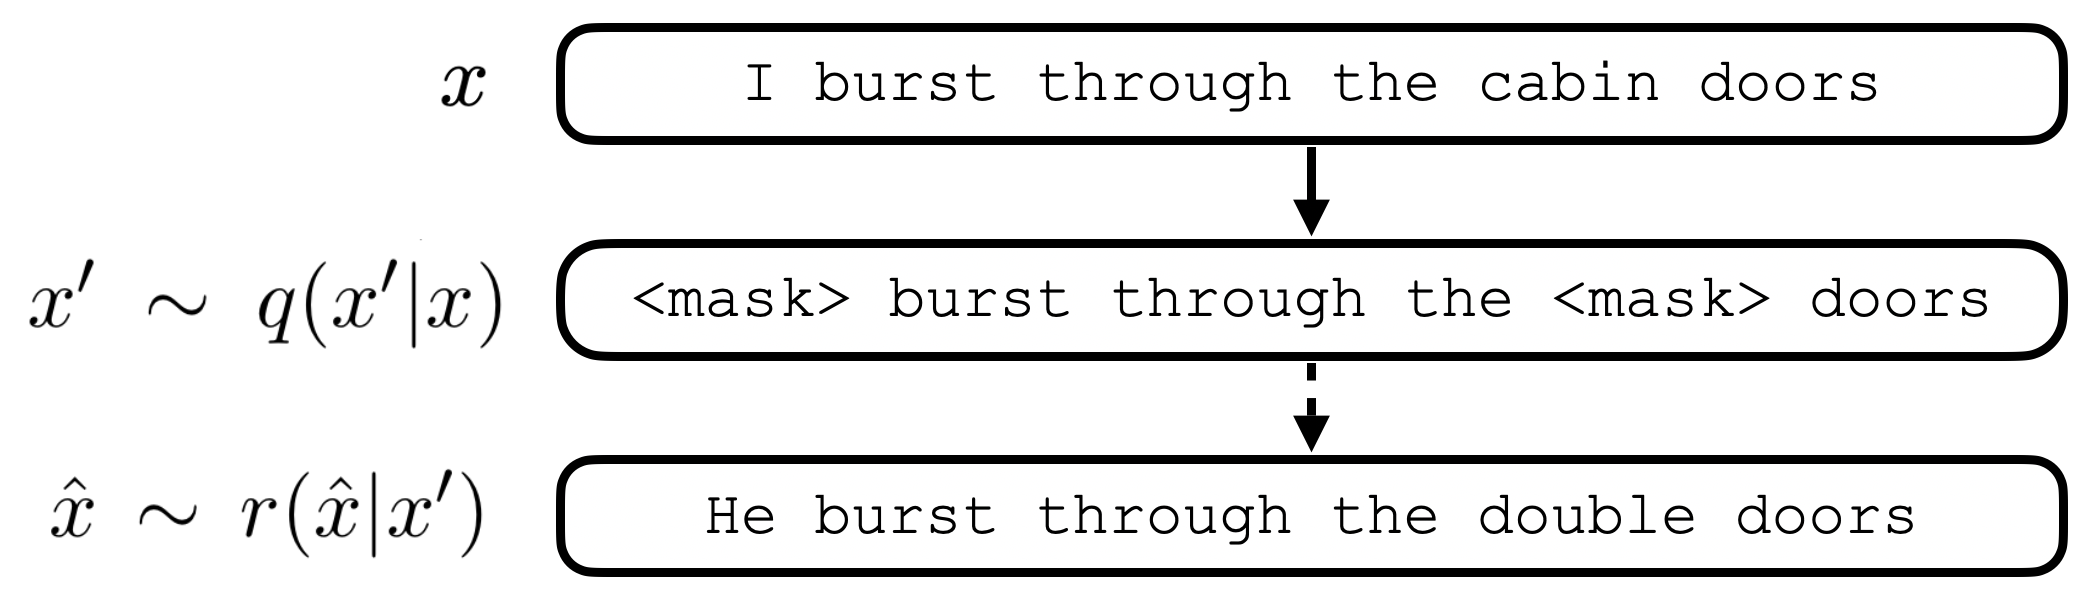
\includegraphics[scale=0.21]{img/bert_dae.png}
\caption{To sample from an MLM DAE, we apply the MLM corruption $q$ to the original sentence then reconstruct the corrupted sentence using our DAE $r$.}
\label{fig:dae_sampling}
\end{figure}

\subsection{Sampling from Denoising Autoencoders}
A denoising autoencoder (DAE) is an autoencoder trained to reconstruct a clean input $x$ from a stochastically corrupted one $x'\sim q(x'|x)$ by learning a conditional distribution $P_\theta (x| x')$ \citep{vincent2008extracting}.
We can sample from a DAE by successively corrupting and reconstructing an input using the following pseudo-Gibbs Markov chain: $x_t' \sim q(x'|x_{t-1})$, $x_t \sim P_\theta(x|x'_t).$
\comment{
\begin{align*}
    x_t' &\sim q(x'|x_{t-1})\\
    x_t &\sim P_\theta(x|x'_t) 
\end{align*}
}
As the number of training examples increases, the asymptotic distribution $\pi_n(x)$ of the generated samples approximate the true data-generating distribution $P(x)$ \citep{bengio2013generalized}.
This corruption-reconstruction process allows for sampling directly along the manifold that $P(x)$ concentrates on.

\subsection{Masked Language Models}
Recent advances in unsupervised representation learning for natural language have relied on pre-training models on a \textit{masked language modeling} (MLM) objective \citep{devlin2018, liu2019roberta}.
In the MLM objective, a percentage of the input tokens are randomly corrupted and the model is asked to reconstruct the original token given its left and right context in the corrupted sentence.
We use MLMs as DAEs \citep{lewis2019bart} to sample from the underlying natural language distribution by corrupting and reconstructing inputs (Figure \ref{fig:dae_sampling}).

% \begin{table}[h]
    % \captionsetup{font=small}
    \small
    \centering
    % \vspace{-1em}
    \caption{\label{table:synthetics} Evaluation of 2-layer models on synthetic language tasks.}
    %   \vspace{1em}
    {
        \begin{tabular}{@{}|c|c|ccc|c|@{}}
        %   \specialrule{.15em}{.05em}{.05em}
        \hline
        Task & Random & S4D & Gated State Spaces & H3 & Attention  \\ % & Training time \\
        %   \specialrule{.15em}{.05em}{.05em}
        \hline
        Induction Head & 5.0 & 35.6 & 6.8 & \textbf{100.0} & \textbf{100.0} \\
        Associative Recall & 25.0 & 86.0 & 78.0 & 99.8 & \textbf{100.0}  \\ \hline
        % Gated State Spaces & 78.0 & 6.8 & 88.2 \\
        % LSTM & -- & -- & -- \\
        % H3 & 99.8 & \textbf{100.0} & \textbf{99.6}  \\ \hline
        % Attention & \textbf{100.0} & \textbf{100.0} & 71.0 \\ \hline
        \end{tabular}
    }
    % \vspace{-1.5em}
\end{table}

% \begin{table}[h]
%     % \captionsetup{font=small}
%     \small
%     \centering
%     % \vspace{-1em}
%     \caption{\label{table:synthetics} Evaluation of 2-layer GPT models on in-context learning synthetic tasks.}
%     %   \vspace{1em}
%     {
%         \begin{tabular}{@{}|c|ccc|@{}}
%         %   \specialrule{.15em}{.05em}{.05em}
%         \hline
%         Model & Associative Recall & Induction Head & Partial Copy  \\ % & Training time \\
%         %   \specialrule{.15em}{.05em}{.05em}
%         \hline
%         Random & 50.0 & 5.0 & 5.0 \\
%         S4D & 86.0 & 35.6 & 98.5  \\
%         Gated State Spaces & 78.0 & 6.8 & 88.2 \\
%         % LSTM & -- & -- & -- \\
%         H3 & 99.8 & \textbf{100.0} & \textbf{99.6}  \\ \hline
%         Attention & \textbf{100.0} & \textbf{100.0} & 71.0 \\ \hline
%         \end{tabular}
%     }
%     % \vspace{-1.5em}
% \end{table}
\begin{figure}[t]
    \centering
    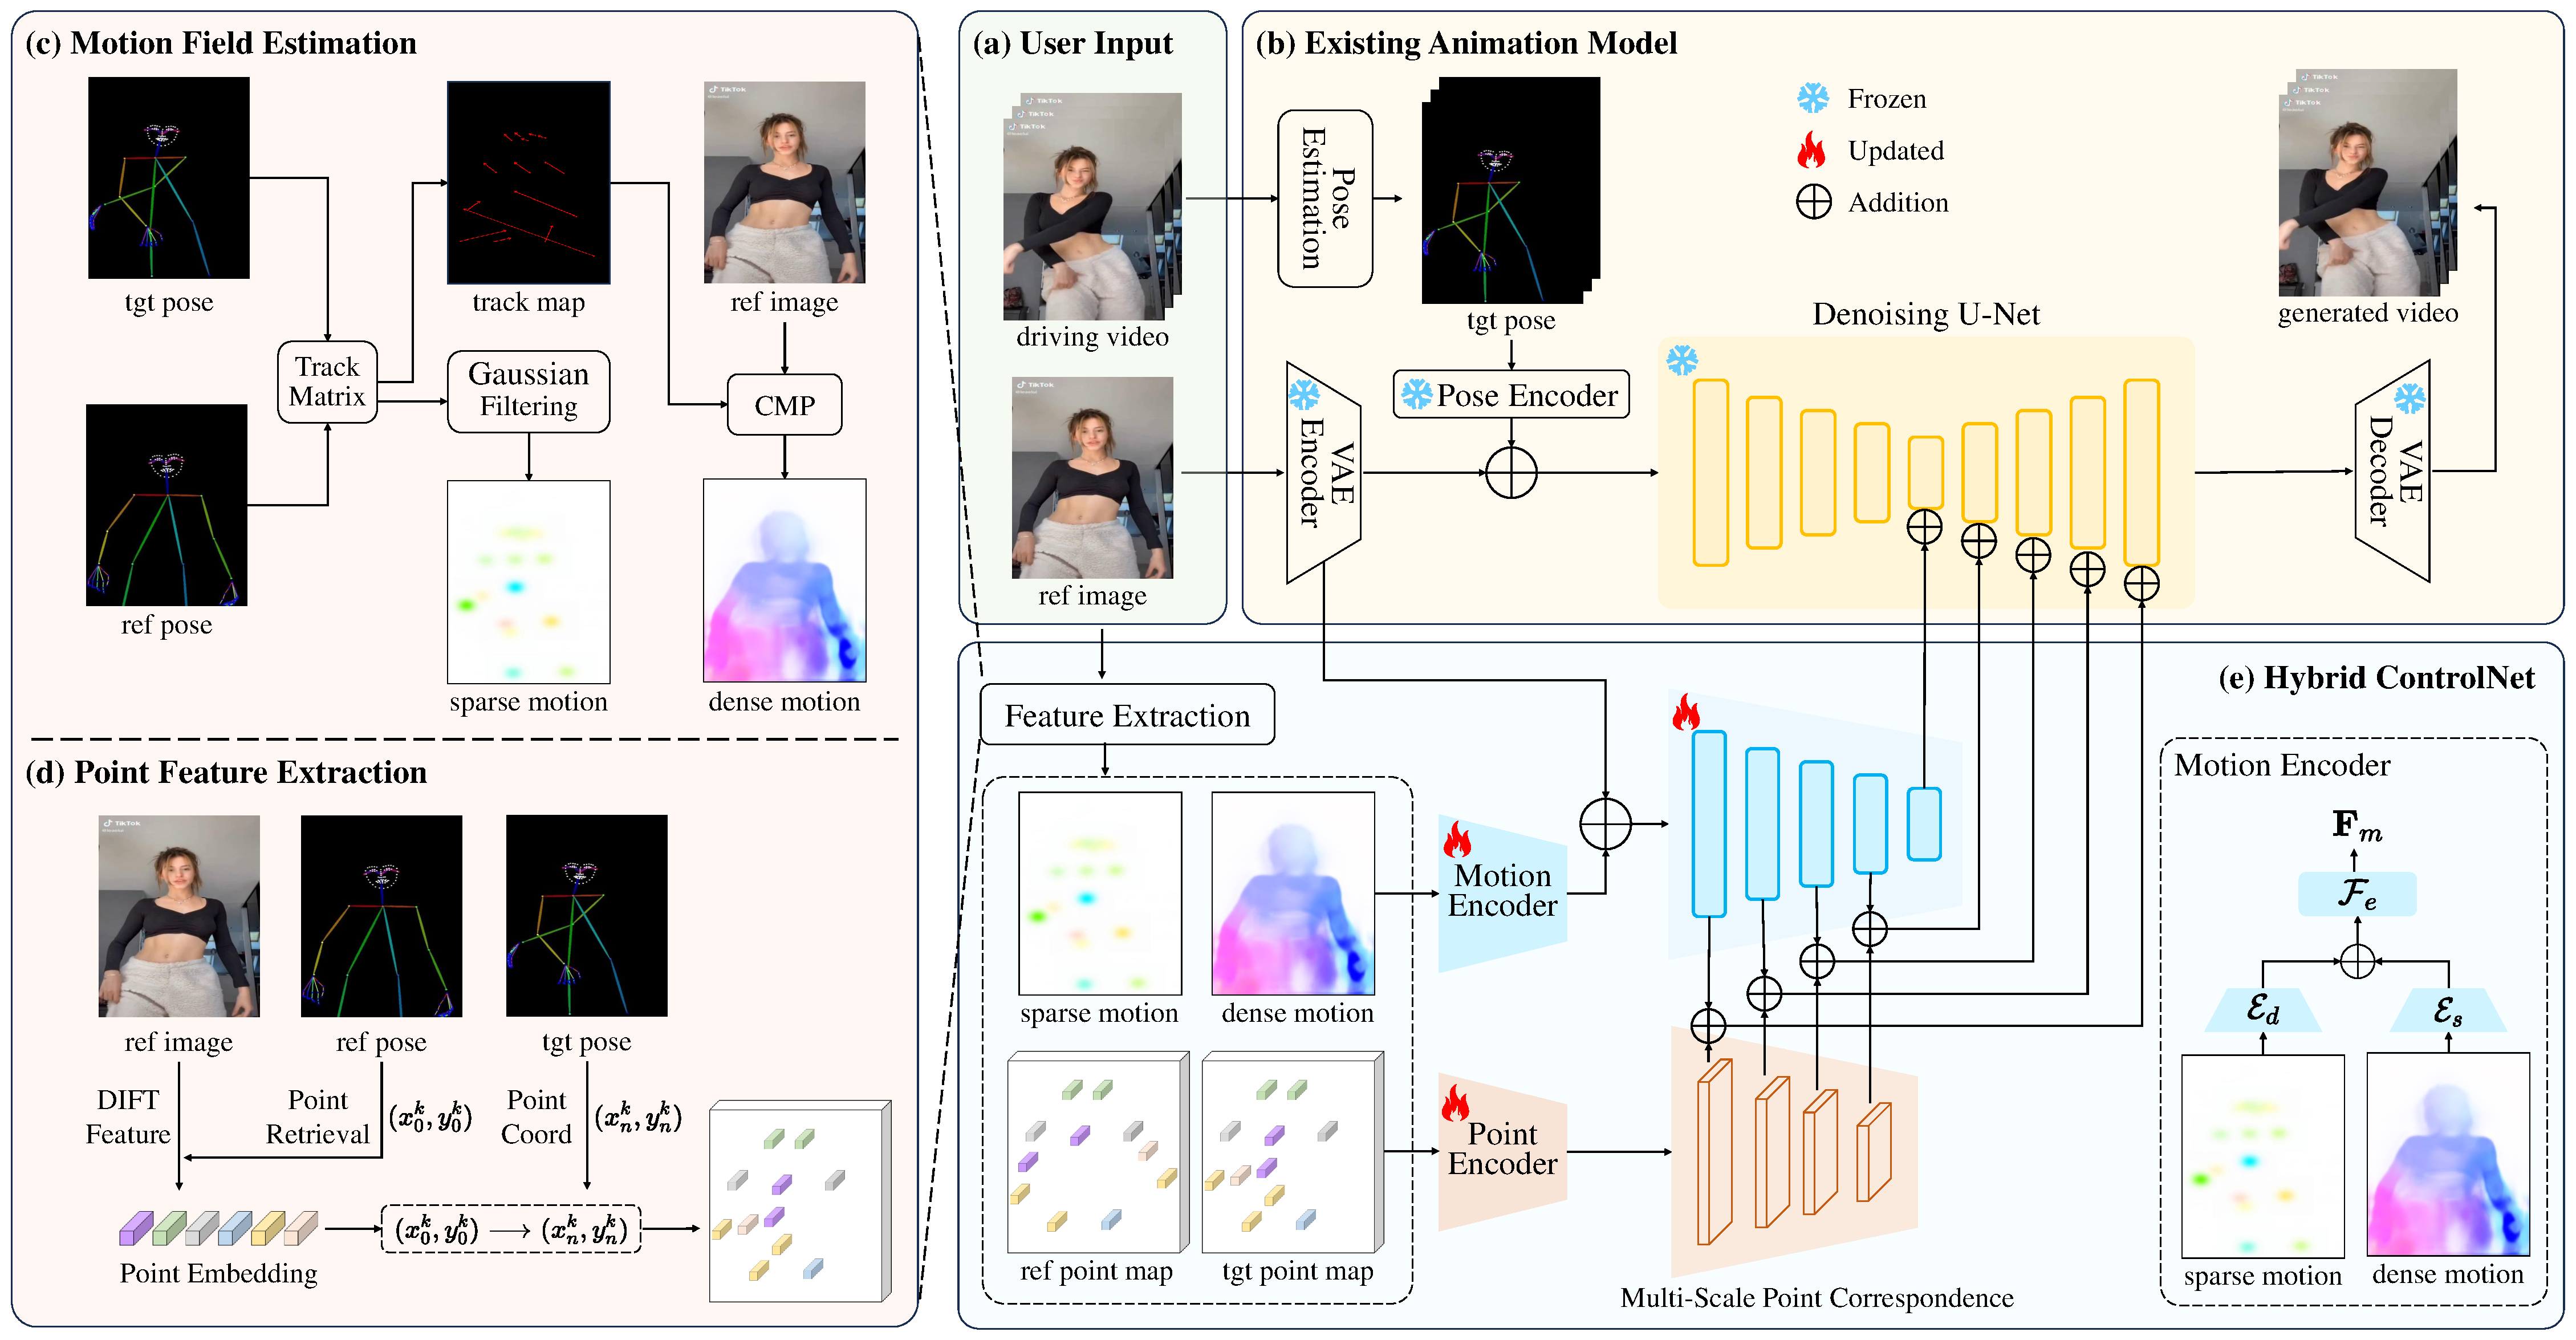
\includegraphics[width=1.0\columnwidth]{./image/pipeline.pdf}
    \vspace{-15pt}
    \caption{The overview of proposed DisPose.}
    \label{fig:pipeline}
\end{figure}
\section{DisPose}
Given a reference image $I_{\mathrm{ref}}\!\in\!\mathbb{R}^{3 \times H \times W}$ and a driving video $V\!\in\!\mathbb{R}^{N\times 3 \times H \times W}$. The core of our method is to disentangle efficient control guidance from only skeleton poses and reference images as shown in Figure~\ref{fig:pipeline}, which can be applied to existing human animation methods without additional dense inputs. We first introduce sparse and dense motion field guides in Sec.~\ref{sec: motion}. Then, we introduce reference-based keypoint correspondence in Sec.~\ref{sec: keypoint}. Finally, we introduce the pipeline of hybrid ControlNet in Sec~\ref{sec: controlnet}.
\subsection{Motion Field Guidance}
\label{sec: motion}

\textbf{Sparse Motion Field.}
We first estimate the skeleton pose by DWpose~\citep{yang2023dwpose} to obtain each frame's human key point coordinates. 
% Subsequently, the motion trajectory of all semantic points in the entire video is obtained and represented as
Subsequently, the key points of the reference image are used as starting points to track the motion displacement of all frames and represented as $P_{traj}\!=\!\{(x^k_n,y^k_n) \!\mid\! k=1\dots K, n=0\dots N\}$, where $P_{traj}$ denotes the trajectory map of the key point $k$ overall $N$ frames and $n = 0$ denotes the reference image. We calculate the track matrix $P_{s}$ as follows:
\begin{equation}
    \mathbf{P}_{s}=\{(x^k_n-x^k_{n-1}, y^k_n-y^k_{n-1}) \mid n=1\dots N\}\},
\end{equation}
% where $P_{t}$ denotes the trajectory map of the key point point $k$ over all $N$ frames, and the reference frame when $n = 0$.
where $K$ denotes the number of keypoints, $N$ denotes the number of frames, $\mathbf{P}_{s}$ denotes the trajectory map of keypoint k over all N frames, and $n = 0$ denotes the reference image.
To avoid training instability caused by overly sparse trajectory matrice, we then apply Gaussian filtering to enhance $\mathbf{P}_{s}$ to obtain the sparse motion field $\mathbf{F}_s\!\in\!\mathbb{R}^{(N-1)\times 2 \times H \times W}$ inspired by~\citep{yin2023dragnuwa, wang2024motionctrl}.

\textbf{Dense Motion Field.}
Considering that sparse control provides limited guidance and dense control is hard to obtain during inference,
% For the dense motion field, 
we transform dense guidance into the motion propagation from the reference frame to the target pose, instead of the dense signal of the target pose. Specifically, in the inference, we reconstruct the trajectory map $\mathbf{P}_{s}$ as the reference-based sparse optical flow $\mathbf{P}_{d}$ from the reference frame to each target pose as:
\begin{equation}
    \mathbf{P}_{d}=\{(x^k_n-x^k_{0}, y^k_n-y^k_{0}) \mid n=1\dots N\}\},
\end{equation}
We then predicted the reference-based dense motion filed $\mathbf{F}_d\!=\! \text{CMP}(P_{traj}, \mathbf{P}_{d}, I_{ref})\!\in\!\mathbb{R}^{(N-1)\times 2 \times H \times W}$ by condition motion propagation (CMP)~\citep{zhan2019self} based on the sparse optical flow $\mathbf{P}_{d}$ and the reference image $I_{ref}$.
CMP~\citep{zhan2019self} is a self-supervised learning-from-motion model that acquires an image and a sparse motion field and estimates the corresponding dense motion field.
Notably, the dense motion field $\mathbf{F}_d$ of each frame starts with the reference image, which avoids geometric constraints during inference.

To ensure motion estimation accuracy during training, we first extract the forward optical flow from the driving video using existing optical flow estimation models~\citep{teed2020raft, xu2023unifying}. We then use a watershed-based approach~\citep{zhan2019self} to sample the sparse optical flow $\mathbf{P}_{d}$ from the forward optical flow. See Appendix.~\ref{sec: appendix1} for details.

\textbf{Motion Encoder.} To leverage motion field as guidance, we introduce a motion encoder specifically designed for the optional flow, which includes sparse motion encoder $\mathcal{E}_s$, dense motion encoder $\mathcal{E}_d$ and feature fusion layer $\mathcal{F}_e$. $\mathcal{E}_d$ and $\mathcal{E}_s$ have the same structure and are multi-scale convolutional encoders with each stage built by \texttt{Conv-SiLU-ZeroConv}~\citep{zhang2023adding} as the basic block. The feature fusion layer $\mathcal{F}_e$ is a 2D convolution for fusing sparse motion features $\mathcal{E}_s(\mathbf{F}_s)$ and dense motion features $\mathcal{E}_d(\mathbf{F}_d)$. Finally, we compute the motion field guidance $\mathbf{F}_m$:
\begin{equation}
    \mathbf{F}_m = \mathcal{F}_e(\mathcal{E}_s(\mathbf{F}_s)+\mathcal{E}_d(\mathbf{F}_d))
\end{equation}

\subsection{Keypoint Correspondence}
\label{sec: keypoint}
\textbf{Point Feature Extraction.} 
To maintain a consistent appearance, it is crucial to correspond the content of the reference image with the motion trajectory. 
Specifically, we first extract the DIFT~\citep{tang2023emergent} features $\mathbf{D}$ of the reference image using the pre-trained image diffusion model. 

Subsequently, the keypoint embedding in the reference is obtained as $\mathbf{D}(x^k_0,y^k_0)$, where $(x^k_0,y^k_0)$ is retrieved from the reference pose.
% key point embeddings $\mathbf{D}(x^k_0,y^k_0)$ are retrieved from $\mathbf{D}$ by skeleton pose $(x^k_0, y^k_0)$.
Next, we initialize the keypoint correspondence map $\mathbf{F}_p$ with zero vectors and assign point embeddings according to the trajectory coordinates as:
\begin{equation}
\label{eq: v prob}
f^{ij}_n=\left\{\begin{array}{ll}
\mathbf{D}(x^k_0,y^k_0), & \mathrm{if} \quad i=x^k_n, j=y^k_n,  \\
0, & \mathrm{otherwise}.
\end{array}\right.
\end{equation}

Finally, we obtain the keypoint correspondence map $\mathbf{F}_p=\{f_n\!\mid\!n=1\dots N\} \!\in\!\mathbb{R}^{N\times D_p \times H \times W}$ for all frames, where $D_p$ is the feature dimension of the point embedding.

\textbf{Point Encoder.} 
To utilize the content correspondence of key points as guidance, we generate multi-scale correspondences of sparse point feature maps and make them compatible with the U-Net encoder of the {Hybrid ControlNet (Sec.4.3)}. 
% as detailed in F. 1.
We introduce the multi-scale point encoder $\mathcal{E}_p$ to maintain the key point content $\mathbf{F}_p$ from the reference image. The point encoder $\mathcal{E}_p$ consists of a series of learnable MLPs.
{
To seamlessly integrate into existing models, we extract intermediate features of the encoder of the hybrid Controlnet.
The multi-scale intermediate features of the Controlnet encoder are denoted as $\mathbf{E}^l_{enc}$, where $l$ denotes each U-Net block $l\!\in\![1, L]$.}
To match the spatial size of $\mathbf{E}^l_{enc}$, we apply downsampling to the feature map between the encoder layers. We compute the multi-scale keypoint correspondence as follows:
\begin{equation}
    \mathbf{F}_c^l = \mathcal{E}_p^l(\phi(\mathbf{F}_p, H^l, W^l)),
\end{equation}
where $(H^l, W^l)$ are denote the spatial dimension of the $l$-th U-Net block and $\phi$ means downsampling operation. Therefore, $\mathbf{F}_c^l$ shares the same size as $\mathbf{E}^l_{enc}$.
Finally, $\mathbf{F}_c$ are added elementwisely to the intermediate feature $\mathbf{E}^l_{enc}$ of the U-Net encoder as guidance: $\mathbf{E}^l_{enc}\!=\!\mathbf{E}^l_{enc}+\mathbf{F}_c^l$.


\subsection{Plug-and-play Hybrid ControlNet}
\label{sec: controlnet}
After obtaining motion field guidance and keypoint correspondence, we aim to integrate these control guidance seamlessly into the U-Net architecture of existing animation models.
Inspired by ControlNet~\citep{zhang2023adding}, We design a hybrid ControlNet $\mathcal{F}$ to provide additional control signals for the existing animation model as shown in Figure~\ref{fig:pipeline}(e).
% Specifically, we consider freeze denoising U-Net and pose encoder. 
Specifically, given an animation diffusion model based on the U-Net architecture, we freeze all its modules while allowing the motion encoder, point encoder and hybrid ControlNet to be updated during training. 
Subsequently, $\mathbf{F}_m$ is added to the noise latent before being input into the hybrid ControlNet. Considering the high sparsity of the point feature $\mathbf{F}_c$, we correspondingly add $\mathbf{F}_c$ to the input of the convolutional layer. Notably, the U-Net encoder intermediate feature $\mathbf{E}_{enc}$ in Sec.~\ref{sec: keypoint} is from hybrid ControlNet rather than denoising U-Net. Finally, 
the control condition is computed as:
\begin{equation}
    \boldsymbol{r}=\mathcal{F}(\boldsymbol{z}_{{t}} \mid \mathbf{F}_m, \mathbf{F}_c, {t})
\end{equation}
where $\boldsymbol{r}$ is a set of condition residuals added to the residuals for the middle and upsampling blocks in the denoising U-Net.
\section{\hthree Evaluation}
\label{sec:evaluation}

\begin{table}[t]
    % \captionsetup{font=small}
    \small
    \centering
    % \vspace{-1em}
    \caption{\label{table:gpt} Perplexity (lower is better) of models on the Pile, OpenWebText and
      WikiText-103. GPT-Neo and hybrid \hthree are trained on the Pile, while GPT2 is
      trained on WebText. All models use the same GPT2 tokenizer. We report the
      perplexity of GPT-2 models on the Pile ($^*$) for context, though the performance is not directly comparable since they were trained on different data.}
  %   \vspace{1em}
    {
      \begin{tabular}{@{}|c|c|cc|@{}}
      %   \specialrule{.15em}{.05em}{.05em}
      \hline
        Model & Pile & OpenWebText & WikiText103 \\ % & Training time \\
      %   \specialrule{.15em}{.05em}{.05em}
        \hline
        % GPT-2 small (125M) & 9.8 & 18.2 & -- \\ % & 4.7 days \\
        % H3 (126M) & 18.7 & 4.5 days \\ \hline
        % OPT-125M & -- & -- & -- \\
        GPT-2 small (125M) & 19.0* & 22.6 & 29.9 \\
        GPT-Neo-125M & 9.4 & 22.6 & 26.3 \\
        % GPT3-125M (our replication) & - & - & 24.6 \\
        \textbf{Hybrid H3-125M} & \textbf{8.8} & \textbf{20.9} & \textbf{23.7} \\ \hline %2.7 days \\ \hline
        GPT-2 medium (355M) & 13.9* & 17.0 & 21.8 \\ % & 11.5 days \\
        % H3 (361M) &  &  \\ \hline
        % OPT-350M & -- & -- & -- \\
        % GPT3-355M (our replication) & - & - & 16.6 \\
        \textbf{Hybrid H3-355M} & \textbf{7.1} & \textbf{15.9} & \textbf{16.9} \\ \hline
        GPT-2 XL (1.5B) & 12.4* & 12.9 & 17.0 \\
        % OPT-1.3B & -- & -- & -- \\
        GPT-Neo-1.3B & 6.2 & 13.1 & 13.3 \\
        \textbf{Hybrid H3-1.3B} & \textbf{6.0} & \textbf{12.4} & \textbf{12.5} \\
        \hline
        GPT-Neo-2.7B & 5.7 & 11.7 & 11.5 \\
        \textbf{Hybrid H3-2.7B} & \textbf{5.4} & \textbf{11.0} & \textbf{10.6} \\
        \hline
      \end{tabular}
    }
    % \vspace{-1.5em}
  \end{table}

\begin{table}[t]
    % \captionsetup{font=small}
    \scriptsize
    \centering
    % \vspace{-1em}
    \caption{\label{table:superglue_zeroshot_logit} Zero-shot acc.\ on SuperGLUE with logit scoring. Best results in bold, second best underline. }
    %   \vspace{1em}
    {
        \begin{tabular}{@{}|c|cccccccc|c|@{}}
            \hline
        %   \specialrule{.15em}{.05em}{.05em}
        Model & WSC & WIC & RTE & CB & MultiRC & ReCoRD & BoolQ & COPA & Average \\ % & Training time \\
        %   \specialrule{.15em}{.05em}{.05em}
        \hline
        % GPT-2 small (125M) & -- & -- & -- & -- & -- & -- & -- & -- & -- \\ % & 4.7 days \\
        % H3 (126M) & 18.7 & 4.5 days \\ \hline
        OPT-125M & \textbf{39.4} & \underline{52.0} & 48.7 & 37.4 & \underline{58.9} & \underline{44.9} & \underline{59.6} & \underline{60.0} & 50.1 \\
        GPT-Neo-125M & \underline{36.5} & \textbf{53.6} & \underline{53.1} & \underline{41.1} & \textbf{59.9} & 39.6 & \textbf{62.2} & \underline{60.0} & \underline{50.8} \\
        % \textbf{\hthree-125M} & 0.0 & 0.0 & 47.3 & 8.9 & 0.0 & -- & 37.8 & 51.0 & 20.7 \\ %2.7 days \\ \hline
        \textbf{Hybrid \hthree-125M} & \textbf{39.4} & 51.4 & \textbf{59.2} & \textbf{48.2} & 51.4 & \textbf{55.0} & \underline{59.6} & \textbf{67.0} & \textbf{53.9} \\ \hline %2.7 days \\ \hline
        GPT-2 medium (355M) & \underline{50.0} & \textbf{52.0} & 51.3 & 28.6 & \textbf{59.5} & \underline{53.3} & \underline{61.0} & \underline{65.0} & 52.6 \\
        % H3 (361M) &  &  \\ \hline
        OPT-350M & \textbf{53.5} & 50.8 & \underline{53.4} & \underline{35.7} & \underline{58.9} & 51.4 & 60.9 & 60.0 & \underline{53.1} \\
        \textbf{Hybrid \hthree-355M} & 37.5 & \underline{51.7} & \textbf{55.2} & \textbf{41.1} & \textbf{59.5} & \textbf{62.3} & \textbf{61.5} & \textbf{69.0} & \textbf{54.7} \\ \hline
        % GPT-2 (1.5B) & 14.4 & \textbf{36.5} & \underline{49.1} & \underline{8.9} & 0.5 & \underline{44.0} & \underline{46.6} & 59.0 & 32.4 \\
        OPT-1.3B & 36.5 & 49.5 & \textbf{53.4} & \textbf{39.3} & \textbf{58.3} & \underline{61.8} & 55.0 & \underline{69.0} & \underline{52.9} \\
        GPT-Neo-1.3B & \underline{41.3} & \underline{50.0} & \underline{52.3} & \underline{33.9} & 57.9 & 55.5 & \underline{59.9} & 66.0 & 52.1 \\
        \textbf{Hybrid \hthree-1.3B} & \textbf{52.9} & \textbf{50.3} & \textbf{53.4} & \underline{33.9} & \underline{58.2} & \textbf{67.8} & \textbf{61.7} & \textbf{74.0} & \textbf{56.5} \\ \hline
        OPT-2.7B & \textbf{51.0} & \underline{50.8} & 50.5 & \underline{41.1} & 57.4 & \underline{65.9} & 60.9 & 66.0 & \underline{55.5} \\
        GPT-Neo-2.7B & \underline{37.5} & 50.0 & \underline{52.3} & \textbf{50.0} & \textbf{59.1} & 60.0 & \textbf{61.1} & \underline{67.0} & 54.6 \\
        \textbf{Hybrid \hthree-2.7B} & 36.5 & \textbf{51.3} & \textbf{57.0} & 37.5 & \underline{58.7} & \textbf{71.3} & \textbf{61.1} & \textbf{81.0} & \textbf{56.8} \\ \hline
        \end{tabular}
    }
    % \vspace{-1.5em}
\end{table}
\begin{table}[t]
    % \captionsetup{font=small}
    \scriptsize
    \centering
    % \vspace{-1em}
    \caption{\label{table:superglue_fewshot_logit} 3-shot acc.\ on SuperGLUE with logit scoring. Best results in bold, second best underline. }
    %   \vspace{1em}
    {
        \begin{tabular}{@{}|c|cccccccc|c|@{}}
            \hline
        %   \specialrule{.15em}{.05em}{.05em}
        Model & WSC & WIC & RTE & CB & MultiRC & ReCoRD & BoolQ & COPA & Average \\ % & Training time \\
        %   \specialrule{.15em}{.05em}{.05em}
        \hline
        % GPT-2 small (125M) & -- & -- & -- & -- & -- & -- & -- & -- & -- \\ % & 4.7 days \\
        % H3 (126M) & 18.7 & 4.5 days \\ \hline
        OPT-125M & 36.5 & \textbf{50.2} & 47.3 & \underline{44.6} & \textbf{57.9} & \underline{44.9} & 41.9 & 60.0 & \underline{47.9} \\
        GPT-Neo-125M & \underline{38.5} & \underline{50.0} & \underline{53.1} & 17.9 & \underline{56.3} & 39.6 & \textbf{62.1} & \underline{60.0} & 47.2 \\
        \textbf{Hybrid \hthree-125M} & \textbf{43.3} & 49.1 & \textbf{58.1} & \textbf{51.8} & 48.9 & \textbf{55.0} & \underline{56.1} & \textbf{67.0} & \textbf{53.7} \\ \hline %2.7 days \\ \hline
        GPT-2 medium (355M) & 36.5 & \textbf{50.5} & \underline{48.0} & 8.9 & 43.5 & \underline{53.3} & 58.8 & \underline{65.0} & 45.6 \\
        % H3 (361M) &  &  \\ \hline
        OPT-350M & \underline{37.5} & \underline{50.0} & 45.8 & \textbf{44.6} & \underline{49.8} & 51.4 & \textbf{61.7} & 60.0 & \underline{50.1} \\
        \textbf{Hybrid \hthree-355M} & \textbf{42.3} & 47.5 & \textbf{50.5} & \underline{28.6} & \textbf{59.7} & \textbf{62.3} & \underline{60.5} & \textbf{69.0} & \textbf{52.6} \\ \hline
        % GPT-2 (1.5B) & \underline{36.5} & 36.5 & \textbf{56.7} & 41.1 & 6.1 & 43.8 & \underline{53.7} & 61.0 & 41.9 \\
        OPT-1.3B & \textbf{44.2} & \textbf{51.1} & \underline{53.4} & 16.1 & \textbf{59.9} & \underline{62.1} & 38.3 & \underline{70.0} & 49.4 \\
        GPT-Neo-1.3B & 35.6 & \underline{50.6} & 47.3 & \textbf{32.1} & \textbf{59.9} & 55.7 & \textbf{61.2} & 67.0 & \underline{51.2} \\
        \textbf{Hybrid \hthree-1.3B} & \underline{36.5} & 49.2 & \textbf{55.2} & \underline{23.2} & \underline{59.3} & \textbf{67.6} & \underline{56.9} & \textbf{76.0} & \textbf{53.0} \\ \hline
        OPT-2.7B & \underline{44.2} & \underline{50.5} & \textbf{53.4} & 17.9 & \underline{59.2} & \underline{66.0} & \textbf{62.0} & \underline{71.0} & \underline{53.0} \\
        GPT-Neo-2.7B & \textbf{49.0} & \textbf{51.9} & \underline{51.6} & \underline{21.4} & 57.0 & 60.0 & 56.0 & 68.0 & 51.9 \\
        \textbf{Hybrid \hthree-2.7B} & 36.5 & 45.6 & 47.3 & \textbf{46.4} & \textbf{59.4} & \textbf{71.1} & \underline{60.6} & \textbf{77.0} & \textbf{55.5} \\ \hline
        \end{tabular}
    }
    % \vspace{-1.5em}
\end{table}

To understand how well capturing the synthetics in Section~\ref{sec:synthetics} translates to language modeling, we train two hybrid hybrid \hthree-attention language models at sizes 125M, 355M, 1.3B, and 2.7B, and we evaluate their performance against Transformers.
The hybrid models match or exceed the quality of Transformers in perplexity and zero/few-shot learning.
We also validate that \hthree models retain strong performance on non-text sequence modeling.
Appendix~\ref{sec:app_additional_experiments} contains additional experiments on more datasets, length extrapolation, and scaling with data.

\subsection{Language Modeling}
\label{subsec:language_modeling}

We compare hybrid \hthree-attention language models against Transformer-based language models.
We evaluate language modeling performance using perplexity, zero-shot learning, and few-shot learning performance.
Hybrid \hthree models outperform Transformers, which suggests that closing the gap between SSMs and attention on the synthetic languages translates to real language modeling capabilities.
We also report the generation speed of hybrid \hthree models compared to Transformers; since SSMs are recurrent models, they can generate tokens \num{2.4$\times$} faster than Transformers.
Appendix~\ref{sec:app_additional_experiments} shows performance of pure \hthree language models on these same evaluation metrics.

\paragraph{Setup}
We train hybrid models at sizes 125M, 355M, 1.3B, and 2.7B on the Pile~\citep{gao2020pile} for 400B tokens.
We compare against checkpoints of equivalent sizes from
Open-AI~\citep{radford2019language} and GPT-Neo\footnote{There
  is no pretrained GPT-Neo at the 350M size.}~\citep{gpt-neo},
from HuggingFace~\citep{wolf-etal-2020-transformers}.


\paragraph{Perplexity}
Table \ref{table:gpt} shows perplexity on the Pile~\citep{gao2020pile}, OpenWebText~\citep{Gokaslan2019OpenWeb}, and WikiText-103~\citep{merity2016pointer}. 
On the Pile, our 125M hybrid model outperforms GPT-Neo, which was also trained on the Pile.
Our hybrid models also outperform GPT-Neo models and GPT-2 models on zero-shot transfer to OpenWebText and WikiText103.
We report the PPL of GPT-2 models for context, though the performance is not directly comparable since they were trained on different data.

\paragraph{Zero- and Few-shot Performance}
We compare the zero- and few-shot performance of hybrid \hthree language models against OPT~\citep{zhang2022opt}, GPT-Neo, and GPT-2 models, where public checkpoints are available.
We report performance with rank classification on the logits of the possible choices (see Appendix~\ref{sec:app_generation} for raw generation).
Table~\ref{table:superglue_zeroshot_logit} reports zero-shot performance on the SuperGLUE benchmark, and Table~\ref{table:superglue_fewshot_logit} reports the 3-shot performance.
Following the perplexity results, the hybrid language models outperform or match the best the Transformer baseline on more than half the tasks.

\begin{table}[t]
\centering
% \begin{table}[h]
    % \captionsetup{font=small}
    \small
    \centering
    % \vspace{-1em}
    \caption{\label{table:training_time} Inference throughput on A100 80GB, 1.3B models.
    Batch size 64, prompt length 512, 1024, or 1536, and generating 128 tokens
    per sequence in the batch (i.e., 64 $\times$ 128 tokens in a batch). Hybrid
    \hthree is up to 2.4$\times$ faster than a Transformer of similar size in inference. The
    difference is larger for longer sequences.}
    %   \vspace{1em}
    {
        \begin{tabular}{@{}|c|c|c|c|@{}}
            \hline
        %   \specialrule{.15em}{.05em}{.05em}
        Tokens/s & Prompt length 512 & Prompt length 1024 & Prompt length 1536 \\ % & Training time \\
        %   \specialrule{.15em}{.05em}{.05em}
        \hline
        Transformer-1.3B & 1340 & 770 & 520 \\
        % GPT-2 Small (FlashAttention~\citep{dao2022flashattention}) & -- & -- \\ 
        % GPT-2 Small (FasterTransformer~\citep{}) & N/A & -- \\ \hline
        Hybrid \hthree-1.3B & 1980 & 1580 & 1240 \\ \hline
        \end{tabular}
    }
    % \vspace{-1.5em}
% \end{table}
\end{table}
\paragraph{Language Modeling Inference}
Finally, since SSMs are recurrent models, they admit faster text generation than Transformers.
Table~\ref{table:training_time} shows inference throughput of a 1.3B-parameter hybrid model compared to a Transformer.
The hybrid model has up to \num{2.4$\times$} higher throughput.



%%% Local Variables:
%%% mode: latex
%%% TeX-master: "../main"
%%% End:

\begin{figure}
    \centering
    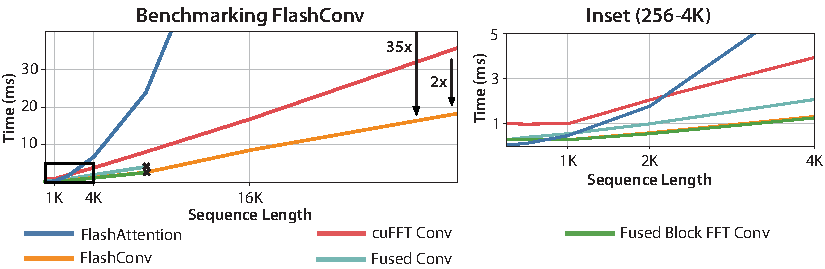
\includegraphics[width=\textwidth]{figs/benchmark_pdf.pdf}
    \caption{\label{fig:fftconv_speed}
      We compare the speed of different algorithms to perform FFT-based
      convolution, along with FlashAttention~\citep{dao2022flashattention} (the fastest attention
      implementation we know of).
      We use batch size 8, hidden dimension 1024, and varying sequence length
      from 256 to 32k, and measure on an A100-SMX4-40GB GPU.
      We see that kernel fusion gives up to 3.4$\times$ speedup over naive FFTConv
      for short sequences (up to 512), block FFT gives up to 2$\times$ speedup for
      medium length sequences (1k - 8k), and state-passing allows 2.3$\times$ faster
      FFTConv for long sequences (16k and above).
    }
\end{figure}
%!TEX root = ../main.tex

\section{Conclusion}
\label{sec:conc}

Our main goal is to understand and narrow the gap between attention and SSMs in
language modeling in terms of modeling capabilities and hardware efficiency.
Our exploration based on synthetic language tasks motivated us to design the
\hthree layer, which is surprisingly competitive with attention.
Our \textsc{BlockFFTConv} algorithm exploits matrix multiplication units and the
dual recurrent--convolution view of SSMs to substantially speed up SSMs, reducing
the hardware barrier between attention and SSMs.
We are excited about several future directions.
Our \hthree layer is a simple combination of two SSMs, and more
sophisticated designs could be more expressive.
Our encouraging results on language models up to 1.3B parameters suggests that
scaling SSMs to larger sizes is a promising avenue.
Since simply adding two attention layers to \hthree models already
outperforms both the pure \hthree model and Transformers, we are optimistic
about combining the complementary strengths of SSMs and attention in the future.

% \pagebreak
\ifarxiv

\else
\textbf{Reproducibility Statement.} To facilitate the reproducibility of our
algorithms and results, (i) we include a link to downloadable source code in
supplementary materials, (ii) for our theoretical statements and results, we
include clear explanations of any assumptions and a complete proof of the claims
in~\cref{sec:proofs}; for any datasets used in the experiments, a complete description of the data processing steps is in~\cref{sec:app_exp_details}.
We will also release model checkpoints for all our models.

\textbf{Ethics Statement.}
Our work seeks to understand the fundamental capabilities and limitations of newly-emerging model architectures.
As the amount of data and model size grows, we also week to understand how to make training these models more efficient---and run inference more efficiently.
This potentially connects to energy savings during model development and deployment.
We also note that the relative underutilization of tensor cores in the FFT convolutions of state space models (even with our block FFT) suggests that consumer GPUs may be able to train models at a cheaper price point.

However, as with any language model training, developing new techniques may impact a wide range of applications, each with potential benefits and harms.
For example, making language model training cheaper and making inference more efficient make it cheaper to spread disinformation.
Similarly, improving the efficiency of model training may not reduce the overall environmental footprint of training, since the same resources may be used to train more models, or train the same models for longer.
While our work makes partial progress on the fronts of efficiency and understanding, it does not explicitly address the issues of fairness and bias in language models.
\fi
%%% Local Variables:
%%% mode: latex
%%% TeX-master: "../main"
%%% End:


\section*{Acknowledgments}

We thank Albert Gu for helpful discussion regarding the model architecture, and
more importantly for sending us daily hippo videos.
We thank Together Computer
for providing portions of the compute used to train models in this paper.
We gratefully acknowledge the support of NIH under No. U54EB020405 (Mobilize), NSF under Nos. CCF1763315 (Beyond Sparsity), CCF1563078 (Volume to Velocity), and 1937301 (RTML); ARL under No. W911NF-21-2-0251 (Interactive Human-AI Teaming); ONR under No. N000141712266 (Unifying Weak Supervision); ONR N00014-20-1-2480: Understanding and Applying Non-Euclidean Geometry in Machine Learning; N000142012275 (NEPTUNE); NXP, Xilinx, LETI-CEA, Intel, IBM, Microsoft, NEC, Toshiba, TSMC, ARM, Hitachi, BASF, Accenture, Ericsson, Qualcomm, Analog Devices, Google Cloud, Salesforce, Total, the HAI-GCP Cloud Credits for Research program,  the Stanford Data Science Initiative (SDSI),
Department of Defense (DoD) through the National Defense Science and
Engineering Graduate Fellowship (NDSEG) Program, 
Wu Tsai Neuroscience Stanford Interdisciplinary Graduate Fellowship,
and members of the Stanford DAWN project: Facebook, Google, and VMWare. The U.S. Government is authorized to reproduce and distribute reprints for Governmental purposes notwithstanding any copyright notation thereon. Any opinions, findings, and conclusions or recommendations expressed in this material are those of the authors and do not necessarily reflect the views, policies, or endorsements, either expressed or implied, of DARPA, NIH, ONR, or the U.S. Government.
Atri Rudra’s research is supported by NSF grant CCF-1763481.


\ifarxiv
\bibliographystyle{plain} % arxiv
\else
\bibliographystyle{iclr2023_conference}
\fi
\bibliography{main}

\appendix
\newpage
%!TEX root = ../main.tex

\section{Related Work}
\label{sec:related}

\textbf{State space models} have shown promise in modeling sequential data, including time series data~\citep{gu2022efficiently}, audio~\citep{goel2022s}, and visual data~\citep{nguyen2022s4nd}.
Our model builds off work on simplifying and parameterizing diagonal versions of S4~\citep{gu2022parameterization,gupta2022diagonal, gu2022train}.
Gated state spaces~\citep{mehta2022long} also aim to adapt SSMs to language modeling, but our results suggest that the GSS model does not perform as well as \hthree (or even as well as earlier SSMs like S4D).
The idea to combine SSMs with attention in hybrid models is not new; Mehta et al.~\citep{mehta2022long} also showed that interleaving attention with their GSS layer can improve performance, which we also validate on our OpenWebText experiments.
These positive results suggest that attention and SSMs are complementary, and that hybrid models may be a promising direction for future work.

\textbf{Large language foundation models}~\citep{bommasani2021opportunities} have demonstrated the power of scaling attention-based networks to billions of parameters and training them on trillions of tokens~\citep{hoffmann2022training}.
Understanding the mechanistic basis~\citep{elhage2021mathematical} behind these models may yield insights into better design choices for future models.
These and similar explorations have informed the design of \hthree and our selection of synthetic languages.
A number of recent works have also explored how to address the shortcomings of attention by approximating the attention computation~\citep{wang2020linformer,katharopoulos2020transformers, choromanski2020rethinking,tay2020long, kitaev2020reformer, daras2020smyrf}.
We believe these efforts are complementary to SSMs, and we are excited to see how they can be combined in future work.

\textbf{Linear attention}~\citep{katharopoulos2020transformers} and classical sequence models like RNNs serve as inspiration for \hthree.
Appendix~\ref{app:linear_attention} draws a direct connection between linear attention and LTI systems.
Luo et al.~\citep{luo2021stable} also propose a variant of linear attention that can achieve $O(n \log n)$ scaling in sequence length.
Appendix~\ref{sec:app_additional_experiments} evaluates linear attention on language modeling, and finds that it underperforms exact attention, whereas \hthree outperforms attention.
The multiplicative interactions in \hthree are reminiscent of gating mechanisms in LSTMs~\citep{hochreiter1996lstm} and GRUs~\citep{cho2014properties}, which suggests that architectural lessons from these sequence models may be useful for adapting SSMs to language modeling.
A number of algorithms for scaling attention to longer sequences have also been proposed, such as Transformer-XL~\citep{dai2019transformer}, Reformer~\citep{kitaev2020reformer}, Performer~\citep{choromanski2020rethinking}, and Perceiver AR~\citep{hawthorne2022general}.
Some of these approaches underperform exact attention on language modeling, and may be slower in wall-clock speed~\citep{dao2022flashattention}.
A thorough comparison of these alternatives to exact attention and how well they scale in model size and amount of training data is fruitful future work.

\textbf{FFT} algorithms are used in a wide variety of applications, including signal processing~\citep{oppenheim1978applications}, control theory~\citep{brogan1974modern}, and more.
Various algorithms for computing the FFT have existed for decades~\citep{oppenheim2001discrete}.
We hope our work on appealing to these classic algorithms to accelerate new applications such as learned SSMs will inspire future algorithmic exploration, even if hardware is not designed for them~\citep{hooker2021hardware}.

%%% Local Variables:
%%% mode: latex
%%% TeX-master: "../main"
%%% End:

\section{Linear Attention and Time-Varying Systems}
\label{app:linear_attention}

We draw some connections from linear attention to LTI systems and SSMs.

We first present linear attention as a linear time-varying system, and show how converting it to a linear time-invariant system matches \hthree.

\paragraph{Linear time-varying system and linear attention}

In general, a layer in a sequence model takes in a sequence and outputs a
sequence.
Many of these take the form of a linear time-varying system (thanks to the
Picard-Lindelof theorem, nonlinear systems can be approximated by a series of
linear system):
\begin{align*}
  x_i &= \vA_i x_{i-1} + \vB_i u_i, \\
  y_i &= \vC_i x_i + \vD_i u_i.
\end{align*}
This has the same form as SSMs (\cref{sec:background}), except that the matrices
can depend on the timestep.

Recall the form of linear attention from~\cref{sec:background}.
For the purpose of approximation, we ignore the denominator in linear
attention~\cref{sec:background} (i.e., assuming $d_i = 1$).
We see that $S_i$ is just a cumulative sum, satisfying the recurrence $S_{i+1} = S_{i} + \phi(K_{i+1}) V_{i+1}^T$.
Similarly, $O_i$ satisfies the recurrence $O_{i+1} = \phi(Q_{i+1})^T S_{i+1}$.
This is a linear time-varying system of the form $x_{i+1} = \vA x_i + \vB u_{i+1}$ and
$y_{i+1} = \vC_{i+1} x_{i+1}$ (with $\vA = I$, $\vB = I$, $u_{i} = \phi(K_{i}) V_i^T$,
$C_{i} = \phi(Q_{i})^T$).
That is, $\vA$ and $\vB$ are constant, but $C$ is time-variant.

To convert this into a linear time-invariant version, we treat the time-variant $\vC_i$ as a post-processing step.
We instead of a fixed $\vC$ for the LTI.
This yields an LTI:
\begin{align*}
  x_{i+1} &= \vA x_i + \vB \phi(K_{i}) V_i^T, \\
  y_{i+1} &= \vC x_{i},
\end{align*}
for some matrices $\vA, \vB, \vC$ that are learned.
We then apply post-processing by multiply $y_{i+1}$ with $\phi(Q_i)^T$.
Replacing $\phi(K_{i})$ with a shift SSM yields an analogue to \hthree.

\section{Method details}
\label{sec:method_details}

Since we have described the forward pass in~\cref{sec:method}, we describe here
the backward pass in details.

\subsection{Backward Pass}
We show how to compute the backward pass in a fused kernel.


Let $y = f \ast u + \vD u$.
In our case, we have $f$ and $u$ have the same length, so they are symmetric as far as the convolution is concerned.

Suppose we are given $dy = \frac{\partial l}{\partial y}$ (where $l$ is some loss function).
We wish to compute $du$, $df$, and $dD$ (which are $\frac{\partial l}{\partial u}$, $\frac{\partial l}{\partial f}$, and $\frac{\partial l}{\partial \vD}$, respectively).

The most challenging part is computing the gradient through the convolution operator - but we'll see that we can re-use our FFT infrastructure for it.
The rest of the operations are straightforward; we have $d\vD = dy u^T$.

\paragraph{Gradient of the Convolution}

Here, we'll discuss how to compute $df$ by integrating w.r.t. the convolution operator $\ast$.
As an immediate consequence, we'll be able to compute $du$ as well.

Since $f$ and $u$ are the same length $L$, $f \ast u$ and $u \ast f$ have the same result.
%  (this is also clear from the FFT convolution rule, since multiplication is commutative).
Thus, we'll start from $u \ast f$ here.

For some notation, let $O = u \ast f$.
Then, $dO = dy$.
Recall that $O[i] = \sum_{j=0}^{i-1} u[i-j]f[j]$.

We'll start by extending $u$ and $f$ with zeros, to give them length $2L$.
Let $u' = [u[0], u[1], \dots, u[L-1], 0, \dots, 0]$, and $f'$ extended similarly.
Let $O' = u' \ast f'$, and $O = O'[:N]$.
Assume that we have all the values of $dO'$ (we only have them for the first half, but we'll see that it doesn't matter in the end).

Let's construct a Toeplitz matrix $H_{u'}$ such that $u' \ast f' = H_{u'} f'$:
$$
H_{u'} = \begin{bmatrix}
  u'[0] & 0     & \dots & 0 \\
  u'[1] & u'[0] & \dots & 0 \\
  \vdots & \vdots & \ddots & \vdots \\
  u'[2L-1] & u'[2L-2] & \dots & u'[0]
\end{bmatrix}
$$
Since, we have $u'[i] = f'[i] = 0$ for $i \geq L$, we can actually fill in the zeros of the above matrix as well:
$$
H_{u'} = \begin{bmatrix}
  u'[0] & u'[2L-1] & \dots & u'[1] \\
  u'[1] & u'[0] & \dots & u'[2] \\
  \vdots & \vdots & \ddots & \vdots \\
  u'[2L-1] & u'[2L-2] & \dots & u'[0]
\end{bmatrix}
$$
Then, we can use the matrix multiplication chain rule to find that:
\begin{align*}
df' = H_{u'}^T dO' &= \begin{bmatrix}
  u'[0] & u'[1] & \dots & u'[2L-1] \\
  u'[2L-1] & u'[0] & \dots & u'[2L-2] \\
  \vdots & \vdots & \ddots & \vdots \\
  u'[1] & u'[2] & \dots & u'[0]
\end{bmatrix} \\
&= \begin{bmatrix}
  u'[0] & u'[-(2L-1)] & \dots & u'[-1] \\
  u'[-1] & u'[0] & \dots & u'[-2] \\
  \vdots & \vdots & \ddots & \vdots \\
  u'[-(2L-1)] & u'[-(2L-2)] & \dots & u'[0]
\end{bmatrix},
\end{align*}
where we use $u'[-i]$ to mean $u'[2L - i]$.
Notice that this matrix has the same format as $H_{u'}$!
Let $u_*' = [u'[0], u'[-1], \dots, u'[-(2N-1)]]$.
Then:
$$
df' = (u_*' \ast dO').
$$
So how do we compute $u_*'$ efficiently?
Naively, we might incur some nasty memory access issues.
But a nice property about the DFT saves us!

Let $U[i]$ be the $i$-th element of the DFT of a signal $u$.
Note that $U[i]$ is complex.
We have:
$$
U^*[i] = U[-i],
$$
where here the $*$ represents the complex conjugate.
We can use this property to compute $df'$ efficiently:
$$df' = u_*' \ast dO'= iFFT(FFT^*(u')FFT(dO')) \Rightarrow df = df'[:N] = iFFT(FFT^*(u')FFT(dy'))[:N],$$
where $FFT^*$ denotes taking the complex conjugate of the FFT, and $dy'$ denotes $dy$, padded with zeros.

\paragraph{Computing $du$}
We can use this same trick to compute $du$, except we need to add in the contribution from the original $\vD u$ term.
We end up with:
$$du = du'[:N] + \vD dy = iFFT(FFT^*(f')FFT(dy'))[:N] + \vD dy.$$

\subsection{State-Passing Matrices}
\label{sec:state-passing-matrices}

We show how to derive $\vM_{ux}$ for the state update in our state-passing algorithm.

We wish to construct a matrix $vM_{ux} \in \mathbb{R}^{m \times N'}$ such that $\vM_{ux}u = \sum_{i=1}^{N'} \vA^{N'-1}\vB u_i$.
Note that $\vA^i \vB \in \mathbb{R}^{d \times 1}$ is a column vector.
We can simply stack these column vectors to form a matrix:
$\vM_{ux} = [\vA^{N'-1}\vB, \vA^{N'-2}\vB, \dots, \vB]$.
%%% Local Variables:
%%% mode: latex
%%% TeX-master: "../main"
%%% End:

\section{Proofs}
\label{sec:proofs}

We show parameterizations of \hthree and attention that solves the associative recall task.
We prove~\cref{thm:h3_complexity} and~\cref{thm:statepassing_correctness}.

\subsection{\hthree Expressivity}
\label{sec:app_expressivity}

This section formally describes a parameterization of \hthree that solves the associative recall task.

\subsubsection{Example Language $\Lambda$}
Consider a simple language with 4 keys and 4 values.
For concreteness, we will use the keys $\{k_1, k_2, k_3, k_4\} = L_K$ and the values $\{v_1, v_2, v_3, v_4\} = L_V$, i.e. our language $L = L_K \cup L_V$.
Given a sequence of key-value pairs with one key at the end, we want a model to generate the value associated with the key at the end.
Assume that the key at the end appeared in the sequence.

More formally, let $N+1$ be the length of the sequence, $N$ even.
The language $\Lambda$ consists of sequences $x \in L^{N+1}$.
Each sequence has an associated mapping $f_x : L_K \rightarrow L_V$.
For each sequence, the odd indices are randomly sampled from $L_K$, for $x_1, x_3, \dots, x_{N-1}$.
The even indices are defined by $f_x$: $x_{2*i} = f_x(x_{2*i-1})$, for $1 \leq i \leq N / 2$.
The last item in the sequence $x_{N+1}$, is randomly drawn from the keys that have appeared in $x$ already, i.e. $x_{N+1} \in \cup{\{x_1, x_3, \dots, x_{N-1}\}}$.
The goal of this language modeling task is to produce $f_x(x_{N+1})$ at the end of the sequence.

\subsubsection{H3 Model to Solve $\Lambda$}
We describe a toy \hthree model that can solve $\Lambda$.

Consider a model consisting of an embedding layer, an \hthree model, and an output projection with softmax.
Recall that $d$ is the dimension of the \hthree model, $m$ is the dimension of its hidden states, and $H$ is the number of heads.
Let $d = 8, m = 2, H = 4$.
Let the embedding layer map each key $k_i$ to the $e_i$ basis vector, and map each value $v_i$ to the $e_{4+i}$ basis vector.

Let $\vB_{shift}$ and $\vC_{shift}$ denote the parameters of the shift SSM, and $\vA_{diag}$, $\vB_{diag}$, and $\vC_{diag}$ denote the parameters of the diagonal SSM (let $\vD$ be zero for both).
Let $\vB_{shift} = \vB_{diag} = \vC_{diag} = e_1$.
Let $\vC_{shift}$ = $[0 1]$.
Let $\vA_{diag}$ be a diagonal matrix with $1$s along its diagonal for each \hthree.

\begin{remark}
The action of a diagonal SSM parameterized by $\vA_{diag}$, $\vB_{diag}$, and $\vC_{diag}$ is to act as a cumulative sum over all its input.
The action of shift SSM parameterized by $\vB_{shift}$ and $\vC_{shift}$ is to shift its input by one time step.
\end{remark}

Recall that the \hthree layer maps its input to $Q$, $K$, and $V$ by applying $u\vW_Q$, $u\vW_K$, and $u\vW_V$.
Let $\vW_Q$ and $\vW_K$ be the following:
$$
    \vW_Q = \vW_K = \begin{bmatrix}
        1 & 1 & 0 & 0 & 0 & 0 & 0 & 0 \\
        0 & 0 & 1 & 1 & 0 & 0 & 0 & 0 \\
        0 & 0 & 0 & 0 & 1 & 1 & 0 & 0 \\
        0 & 0 & 0 & 0 & 0 & 0 & 1 & 1 \\
        0 & 0 & 0 & 0 & 0 & 0 & 0 & 0 \\
        0 & 0 & 0 & 0 & 0 & 0 & 0 & 0 \\
        0 & 0 & 0 & 0 & 0 & 0 & 0 & 0 \\
        0 & 0 & 0 & 0 & 0 & 0 & 0 & 0 \\
    \end{bmatrix}
$$
Recall that $Q$ and $K$ are split into $H$ heads ($\vQ^{(i)}, \vK^{(i)}$ for $i \in \{1, 2, 3, 4\}$), each of which is sent to an independent \hthree.

\begin{remark}
The action of $\vW_Q$ and $\vW_K$ are to ``assign'' each key to a different \hthree head, i.e., $\vQ^{(i)}_t$ is only non-zero when $x_t = k_i$.
Similarly, $\overline{\vK}^{(i)}_t$ is only non-zero when $x_{t-1} = k_i$ (since $\overline{\vK}_t = \vK_{t-1}$ due to the time delay of the shift SSM).
\end{remark}

Let $\vW_V$ be the following:
$$
    \vW_V = \begin{bmatrix}
        0 & 0 & 0 & 0 & 0 & 0 & 0 & 0 \\
        0 & 0 & 0 & 0 & 0 & 0 & 0 & 0 \\
        0 & 0 & 0 & 0 & 0 & 0 & 0 & 0 \\
        0 & 0 & 0 & 0 & 0 & 0 & 0 & 0 \\
        0 & 0 & 0 & 0 & 0 & 0 & 0 & 0 \\
        0 & 1 & 0 & 1 & 0 & 1 & 0 & 1 \\
        1 & 0 & 1 & 0 & 1 & 0 & 1 & 0 \\
        1 & 1 & 1 & 1 & 1 & 1 & 1 & 1 \\
    \end{bmatrix}
$$
\begin{remark}
The action of this matrix is to encode the input value (as ``binary''), and send it to all \hthree heads.
E.g., $\vV_t^{(1)} = \vV_t^{(2)} = \vV_t^{(3)} = \vV_t^{(4)}$ for all $i$, and $\vV_t^{(i)} = [0, 0] \Leftrightarrow x_t = v_1$, $\vV_t^{(i)} = [0, 1] \Leftrightarrow x_t = v_2$, etc.
\end{remark}

We claim that for $x_{N+1} = k_i$, $\vO_{N+1}^{(i)}$ will be a multiple of the binary encoding of $f_x(k_i)$, and all the other heads of the output $\vO_{N+1}^{(j)}, 1 \leq j \leq 4, j \neq i$, will be zero.
Let the output projection $\vW_O$ be such that, with a non-linearity afterwards, it inverts the binary encoding to produce the embedding of the desired output $f_x(k_i)$.
We will assume such a projection exists, proof left to the reader.

\begin{proposition}\label{thm:h3_expressivity}
    The model described above solves the associative recall problem for the language $\Lambda$.
\end{proposition}

\begin{proof}
Proof sketch.
WLOG, let $x_{N+1} = k_i$.
Then $\vQ^{(i)} = [1, 1]$, but $\vQ^{(j)} = [0, 0]$ for $j \neq i$.
Thus, $\vO^{(j)} = [0, 0]$ for $j \neq i$ due to the multiplicative interaction.

Since $\vQ^{(i)} = [1, 1]$, $\vO^{(i)}$ is the output of the diag SSMs in the \hthree head corresponding to $k_i$ (recall that each head has two independent shift SSMs and two independent diag SSMs).
The output of the diag SSMs are the cumulative sum of all the inputs they have seen in the sequence.

For one of the diag SSMs to see a non-zero input, its preceding shift SSM must have a non-zero output.
The only times $t$ this can happen in the sequence are when $x_{t-1} = k_i$.
But then $x_t = f_x(k_i)$.
Thus, the input to the diag SSMs are precisely the binary encoding of $f_x(k_i)$.
Then the output $\vO^{(i)}$ is a multiple of the binary encoding of $f_x(k_i)$, $\vW_O$ decodes this output to the embedding of $f_x(k_i)$.
\end{proof}

\subsection{Attention Expressivity}
\label{sec:app_attention_expressivity}
We provide an informal sketch of a two-layer attention model that can solve the associative recall task, inspired by the construction of~\citep{olsson2022context}.
The first layer of the attention model outputs the embedding of the previous token in the sequence, and concatenates it with the current token in the sequence.
The second layer compares the current token to the previous token embeddings, and outputs the paired embedding when there is a match---which is exactly the key-value lookup.

The construction proceeds as follows:
\begin{itemize}
  \item In the first layer, let $Q_i$ be mapped to the positional embedding of token $x_{i-1}$ (e.g., $p_{i-1}$ if $p_i$ denotes the positional embedding of token $x_i$), and $K_i$ be mapped to the positional embedding of token $x_i$.
  \item The attention matrix $A$ is computed as $QK^T$, with a causal mask (i.e., $A_{i, j} = 0$ if $j > i$).
  \item Then, $softmax(A)$ approximates the shift matrix (see Section~\ref{sec:method}).
  \item Let $V_i$ be an encoding of token $x_i$, constrained to the first half of the hidden dimension.
  \item Then, for output $O = softmax(QK^T)V$, the first half of the vector $O_i$ is the encoding of token $x_{i-1}$.
  \item In the second layer, assume that you have a skip connection, that maps the encoding of the input token $x_i$ to the second half of the vector $O_i$.
  \item Then, the input to the second layer encodes both $x_{i-1}$ and $x_i$.
  \item In the second layer, let $Q_i$ extract the encoding of $x_i$, and let $K_i$ extract the encoding of $x_{i-1}$.
  \item Apply a causal mask on $QK^T$. Then, the value of $softmax(QK^T)_{i, j}$ is large if $x_i = x_{j-1}$, and $i > j - 1$.
  \item Let $V_i$ extract the encoding of $x_i$.
  \item Then, output $O_i$ is the sum of values $x_j$ such as $x_{j-1} = x_i$. But then $O_i$ is exactly a lookup of the token that came after $x_i$ when it appeared previously in the sequence---which exactly solves associative recall.
\end{itemize}

We note that the above construction requires the ability for the positional encodings to select the previous token based on the dot product and softmax, and for token comparisons through the dot product and softmax.

\subsection{\hthree Complexity}
\label{sec:app_h3_complexity}

We prove~\cref{thm:h3_complexity}, which states that the \hthree layer takes
$O(d^2N + d N \log N)$ time and $O(dN)$ space for sequence length $N$ and hidden
dimension $d$.

\begin{proof}
  We first analyze the time complexity.
  Consider the matrix multiplies in \hthree, where the input $u \in \mathbb{R}^{N \times d}$ is
  multiplied by three weight matrices of size $d \times d$. These take time $O(d^2N)$.
  The output $\vO$ is also multiplied with an output projection weight matrix of
  size $d \times d$, also taking time $O(d^2N)$.
  Therefore the matrix multiplies take time $O(d^2N)$.

  Now consider the two SSMs in \hthree. The first SSM involves a convolution of
  $\vK \in \mathbb{R}^{N \times d}$ (in the $N$-dimension) with a kernel of size $N \times d$.
  This reduces to an FFT, a pointwise multiply, and an inverse FFT (in the
  $N$-dimension).
  This takes time $O(d N \log N)$.
  The second SSM involves $H$ convolutions, inputs of size $N \times d_h \times d_h$,
  along the $N$-dimension.
  This takes time:
  \begin{equation*}
    O(H d_h^2 N \log N) = O(d d_h N \log N) = O(d N \log N),
  \end{equation*}
  where we use the fact that $d_h = d / H$ and that $d_h = O(1)$.
  Therefore the two SSMs take total time $O(d N \log N)$.
  As a result, the \hthree layer takes time:
  \begin{equation*}
    O(d^2N + d N \log N).
  \end{equation*}

  Now we analyze the space complexity.
  The matrix multiplies all take space $O(dN)$.
  The FFTs, pointwise multiplies, and inverse FFTs of the two SSMs takes $O(dN)$
  space and $O(H d_h^2N) = O(dd_hN) = O(dN)$ space.
  Therefore the overall space complexity is $O(dN)$.

\end{proof}


\subsection{State Passing Correctness}
\label{sec:app_statepassing_correctness_proof}

We prove~\cref{thm:statepassing_correctness}.
We assume that the \textsc{BlockFFTConv} algorithm is correct, i.e., the output $y = $\textsc{BlockFFTConv}$(f, u)$ is equal to the output of an SSM with convolution kernel $f$ and input $u$.

\begin{proof}  
Proof by induction on $C$.

\paragraph{Base case:} $C = 1$.
WTS $y = [y^{(1)}]$, $\vM_{xx}x_{N'}^{(0)} + \vM_{ux}u^{(1)} = x_{N}$.

In this case, note that $N = N'$.
Then $y^{(1)} = \vM_{xy}x_{N'}^{(0)} + $\textsc{BlockFFTConv}$(f, u_1) = $\textsc{BlockFFTConv}$(f, u_1)$.
But $u = u_1$, so $y = y^{(1)} = [y^{(1)}]$.

Additionally, by the recursive definition of a state space,
\begin{align*}
 x_{N} &= \vA^{N-1}x_0 + \sum_{i=1}^N \vA^{N-i}\vB u_i \\
 &= \vA^{N'-1}x_0 + \sum_{i=1}^{N'} \vA^{N'-i}\vB u^{(1)}_i \\
 &= \vM_{xy}x_{N'}^{(0)} + [\vA^{N'-1}\vB, \vA^{N'-2}\vB, \dots, \vB]u^{(1)}. \\
 &= \vM_{xy}x_{N'}^{(0)} + \vM_{ux}u^{(1)}.
\end{align*}

\paragraph{Inductive step:} $C > 1$.
Assume that $[y^{(1)}, \dots, y^{(C-1)}] = y[:N'(C-1)]$, and $x_{N'}^{(C-1)} = x_{(C-1)N'}$.
WTS that $y^{(C)} = y[N'(C-1):N'C]$, and $\vM_{xx}x_{N'}^{(C-1)} + \vM_{ux}u^{(C)} = x_{N}$.
Let $t$ denote $N'(C-1)$.

For $i > (C-1)N'$, we have:
\begin{align*}
y_i &= \vC\vA^{i-t}\vB x_{t} + (f \ast [u_{t}, u_{t+1}, \dots, u_{t+N'-1}])_{i-t} + \vD u_i \\
&= \vC\vA^{i-t}\vB x_{t} + (f \ast u^{(C)})_{i-t} + \vD u_i \\
&= \vC\vA^{i-t}\vB x_{t} + \textsc{BlockFFTConv}(f, u^{(C)})_{i-N'} \\
&= (\vM_{xy}x_t + \textsc{BlockFFTConv}(f, u^{(C)}))_{i-N'} \\
&= (\vM_{xy}x_{N'}^{(C-1)} + \textsc{BlockFFTConv}(f, u^{(C)}))_{i-N'} \\
&= y^{(C)}_{i-N'}.
\end{align*}
Thus, $y^{(C)} = y[N'(C-1):N'C]$.

Similarly,
\begin{align*}
x_N &= \vA^{N'-1}x_{(C-1)N'} + \sum_{i=1}^{N'} \vA^{N'-i}\vB u_{i+t} \\
&= \vA^{N'-1}x_{N'}^{(C-1)} + \sum_{i=1}^{N'} \vA^{N'-i}\vB u^{(C)}_i \\
&= \vM_{xx}x_{N'}^{(C-1)} + [\vA^{N'-1}\vB, \vA^{N'-2}\vB, \dots, \vB]u^{(C)} \\
&= \vM_{xx}x_{N'}^{(C-1)} + \vM_{ux}u^{(C)}.
\end{align*}
\end{proof}
%%% Local Variables:
%%% mode: latex
%%% TeX-master: "../main"
%%% End:

\section{Experimental Details \label{sec:app_exp_details}}

\subsection{Synthetics}
Our synthetic tasks, inspired by~\citep{olsson2022context}, are designed to mimic the in-context learning capability of large language models---the ability to learn from examples in the input sequence, and use information from the input to generate the right answer for the output.
For example, the induction head task requires memorizing the token that appears after the special $\vdash$ token in the input sequence, and the associative recall task requires learning the mapping from keys to tokens from the input sequence.

We evaluate synthetics by training two-layer versions of our GPT models, with different modules replacing attention.
We train models with inner dimension 32, and MLP dimension 128.
For all the synthetics, we use a learning rate of 5e-4 and a weight decay of 0.1.
We sample 5000 training examples and 500 test examples from the same distribution, and we train for 200 epochs.
Again, we use embedding dropout of 0.1 and residual dropout of 0.0.

\subsection{Model Architecture}
For our 125M models, we use 12 layers, with hidden dimension 1024, and MLP dimension 4096.
For our 355M models, we use 24 layers, with the same hidden dimension and MLP dimension.
The 1.3B models have 24 layers, with hidden dimension 2048, and MLP dimension 8192.
The 2.7B models have 32 layers, hidden dimension 2560, and MLP dimension 10240.
The hybrid models have 12, 16, 16, and 20 heads for the 125M, 355M, 1.3B, and 2.7B models, respectively.
The 125M hybrid model has an attention layers at layers 1 and 7, the 355M and 1.3B hybrid models have attention layers at layers 1 and 13, and the 2.7B hybrid model has attention layers at layers 10 and 21.
For both our hybrid models and our \hthree models, we use SSM state size 64.
Our hybrid model uses head dimension 1 for \hthree, while our pure \hthree model uses head dimension 8.
We run models with mixed-precision training, with bf16 for the MLP's and attention.
When training language models, we use fp32 for the FFTConv.

\subsection{OpenWebText Training}
For the 125M models trained on OpenWebText, we follow the training recipe of the Megatron-LM repo.

We use an effective batch size of 512, and use gradient accumulation to fit into
available GPU memory.
We use the AdamW optimizer, with learning rate 6e-4 for GPT-2 small and 1.5e-4
for GPT-2 medium, and weight decay of 0.1.
All models are trained with the same hyperparameters for 100K steps.
We run all implementations with mixed-precision training (PyTorch AMP).
We train models with sequence length 1024.

We use the Openwebtext dataset, with the GPT-2 BPE tokenizer. We randomly select
0.5\% of the dataset as the validation set, with the rest being used as training
set.
This random selection of validation set is done once, and all models are evaluated
on the same validation set.

\subsection{The Pile Training}
For the 125M and 355M models trained on the Pile, we follow the training recipe of GPT-3.
We use batch size 256, with sequence length 2048.
We train our models for 800K steps.
We use residual dropout 0.0 and embedding dropout 0.1.
We use the AdamW optimizer, with learning rate 6e-4 for the 125M model and 3e-4 for the 355M model, and a weight decay of 0.1.
We use a cosine schedule with 8000 steps for linear warmup, and decay the
learning rate to 10\% by 300B tokens, then continue training at 10\% learning
rate for another 100B tokens.
We suspect that there exist better hyperparameters for \hthree language models, but we did not have the resources to tune them.

For the 1.3B models, we double the batch size to 512 (with sequence length
2048), again following the training recipe of GPT-3. The number of training
steps are halved so that we train on the same number of tokens.

For the Pile dataset, we again use the GPT-2 BPE tokenizer, similar to GPT-3 and GPT-Neo.

\subsection{SuperGLUE}
We follow the prompts used in the GPT-3 paper~\citep{brown2020language}.
For rank classification on the binary classification tasks, we use yes/no for WSC, WIC, MultiRC, and BoolQ, and we use true/false for RTE.
For CB, we use true/false/neither as the three choices.
For COPA and ReCoRD, we use the continuations provided by the task.

\subsection{Hardware}
All models were trained on either a single 16xA100-40GB node or a cluster of 8xA100-80GB nodes.

\section{Additional Experiments}
\label{sec:app_additional_experiments}

\subsection{LRA Accuracy}
We evaluate the accuracy of \hthree on LRA.
We compare accuracy to S4D~\citep{gu2022parameterization}, since \hthree uses an S4D kernel as a component in its layer.
We use the same hyperparameters as S4D, and make the layer bidirectional by making two copies and running them in opposite directions.

\begin{table}[ht]
    % \captionsetup{font=small}
    \small
    \centering
    % \vspace{-1em}
    \caption{\label{table:lra_acc} LRA performance of \hthree compared to S4D. }
    %   \vspace{1em}
    {
        \begin{tabular}{@{}|c|cccccc|c|@{}}
            \hline
        %   \specialrule{.15em}{.05em}{.05em}
        Model & ListOps & Text & Retrieval & Image & Pathfinder & Path-X & Avg  \\ % & Training time \\
        %   \specialrule{.15em}{.05em}{.05em}
        \hline
        % GPT-2 small (125M) & -- & -- & -- & -- & -- & -- & -- & -- & -- \\ % & 4.7 days \\
        % H3 (126M) & 18.7 & 4.5 days \\ \hline
        S4D~\citep{gu2022parameterization} & \textbf{58.3} & 87.3 & 90.7 & \textbf{87.5} & \textbf{93.6} & \textbf{92.3} & \textbf{85.0} \\
        \hthree & 57.5 & \textbf{88.2} & \textbf{91.0} & 87.3 & 93.0 & 91.8 & 84.8  \\ \hline
        \end{tabular}
    }
    % \vspace{-1.5em}
\end{table}

Table~\ref{table:lra_acc} shows that \hthree performs well on the LRA benchmark, even thought it was designed for autoregressive language modeling.
\hthree outperforms S4D on two of the LRA tasks, and comes within 1 point on the others.

\subsection{WikiText103}
We train 125M-sized models on WikiText103~\citep{merity2016pointer} and compare their test PPL to transformers, as well as other variants of efficient or long-range attention.
We use the same hyperparameters and setup as training on OpenWebText.
We also provide results from Transformer-XL and Perceiver AR for context, though the results may not be directly comparable due to differences in model size and tokenizer.

\begin{table}[h]
%   \vspace{-1em}
\caption{\label{table:wikitext103} Test PPL on WikiText103.}
\centering
\small
\begin{tabular}{|c|c|}
\hline
Models &  PPL \\
\hline
Transformer (125M) & 18.6  \\
Hybrid \hthree (125M) & 18.5 \\
Performer (125M)~\citep{choromanski2020rethinking} & 26.8 \\
Reformer (125M)~\citep{kitaev2020reformer} & 26.0 \\
Linear Attention (125M)~\citep{katharopoulos2020transformers} & 25.6 \\ \hline
Perceiver AR (358M)~\citep{hawthorne2022general} & 18.4 \\
Transformer-XL (285M)~\citep{dai2019transformer} & 18.4 \\ \hline
% \specialrule{.15em}{.05em}{.05em}
\end{tabular}
%   }
% \vspace{-1em}
\end{table}

Table~\ref{table:wikitext103} shows that the Hybrid \hthree model is competitive with Transformers of the same size, as well as larger models such as the 358M Perceiver AR and 285M Transformer-XL.
The hybrid \hthree model also significantly outperforms transformers with performer, reformer, and linear attention.

We note that the Transformer-XL and Perceiver AR PPl numbers are from the original papers, and may not be directly comparable to our results.
In particular, they use a tokenizer with a different vocab size, which means that the PPLs are not directly comparable.
In addition, the larger vocab size necessitates a change in the model (adaptive softmax) that may affect performance.
The top five numbers in Table~\ref{table:wikitext103} are trained with the same setup and are directly comparable to each other.

\subsection{PG-19}
We evaluate models trained on the PG-19 dataset~\citep{rae2019compressive}, a natural language dataset comprised of texts from books.
We compare the performance of Hybrid \hthree compared against Transformers and linear attention.
We use the same setup as evaluating on OpenWebText.

\begin{table}[h]
%   \vspace{-1em}
\caption{\label{table:pg19} Test PPL on PG-19.}
\centering
\small
\begin{tabular}{|c|c|}
\hline
Models &  PPL \\
\hline
Transformer (125M) & 17.0  \\
Hybrid \hthree (125M) & 16.2 \\
Linear Attention (125M)~\citep{katharopoulos2020transformers} & 19.1 \\ \hline
\end{tabular}
%   }
% \vspace{-1em}
\end{table}

Table~\ref{table:pg19} shows that Hybrid \hthree outperforms transformers and linear attention.

\subsection{Length Extrapolation}
One property of SSMs is that they can naturally extrapolate to sequence lengths longer than those seen during training.
We use the synthetic associative recall task to demonstrate that \hthree maintains this capability.
To do so, we train a two-layer \hthree model on sequences of length 20 drawn from the associative recall synthetic language.
Then, we evaluate accuracy of the last token prediction on sequences of length 20 and 40.

\begin{table}[h]
%   \vspace{-1em}
\caption{\label{table:length_extrapolation} Accuracy of an \hthree model trained for associative recall on sequences of length 20, evaluated on sequences of length 20 and 40.}
\centering
\small
\begin{tabular}{|c|cc|}
\hline
Models & Acc, seqlen 20 & Acc, seqlen 40 \\
\hline
\hthree & 99.8 & 98.4 \\ \hline
\end{tabular}
%   }
% \vspace{-1em}
\end{table}

Table~\ref{table:length_extrapolation} shows that \hthree maintains accuracy on sequences of length 40, which is twice the length of the training sequences.

\subsection{Scaling in Number of Tokens}
We evaluate how well a Hybrid \hthree model scales with the number of tokens seen during training, compared to a Transformer.
For these experiments, we train a 125M Hybrid \hthree model and a 125M Transformer on the Pile for 5B, 10B, and 15B tokens.
We use a learning rate of 6e-4, adjusting the warmup to be 1\% of the total training time, and adjusting the decay rate to decay the learning rate to 6e-5 by the end of training.

\begin{table}[h]
%   \vspace{-1em}
\caption{\label{table:scaling_tokens} Test PPL on the Pile for models trained with fewer tokens.}
\centering
\small
\begin{tabular}{|c|cc|}
\hline
Train Tokens & Hybrid \hthree (125M) & Transformer (125M) \\
\hline
5B & 11.8 & 12.7 \\
10B & 10.7 & 11.3 \\
15B & 10.2 & 10.7 \\
\hline
\end{tabular}
%   }
% \vspace{-1em}
\end{table}

Table~\ref{table:scaling_tokens} shows the results.
Both the Hybrid \hthree model and Transformer model improve as the number of training tokens increases.

\subsection{\hthree Language Model}
\begin{table}[ht]
    % \captionsetup{font=small}
    \small
    \centering
    % \vspace{-1em}
    \caption{\label{table:superglue_zeroshot_all} Zero-shot performance on SuperGLUE with rank classification. Best results for each model size in bold. }
    %   \vspace{1em}
    {
        \begin{tabular}{@{}|c|cccccccc|c|@{}}
            \hline
        %   \specialrule{.15em}{.05em}{.05em}
        Model & WSC & WIC & RTE & CB & MultiRC & ReCoRD & BoolQ & COPA & Average \\ % & Training time \\
        %   \specialrule{.15em}{.05em}{.05em}
        \hline
        % GPT-2 small (125M) & -- & -- & -- & -- & -- & -- & -- & -- & -- \\ % & 4.7 days \\
        % H3 (126M) & 18.7 & 4.5 days \\ \hline
        OPT-125M & \underline{39.4} & \underline{52.0} & 48.7 & 37.4 & \underline{58.9} & \underline{44.9} & \underline{59.6} & \underline{60.0} & 50.1 \\
        GPT-Neo-125M & 36.5 & \textbf{53.6} & \underline{53.1} & \underline{41.1} & \textbf{59.9} & 39.6 & \textbf{62.2} & \underline{60.0} & \underline{50.8} \\
        \textbf{\hthree-125M} & \textbf{61.5} & 50.0 & \underline{53.1} & \underline{41.1} & 4.6 & 15.8 & 46.4 & 51.0 & 40.4 \\%2.7 days
        \textbf{Hybrid \hthree-125M} & \underline{39.4} & 51.4 & \textbf{59.2} & \textbf{48.2} & 51.4 & \textbf{55.0} & \underline{59.6} & \textbf{67.0} & \textbf{53.9} \\ \hline %2.7 days \\ \hline
        \end{tabular}
    }
    % \vspace{-1.5em}
\end{table}
\begin{table}[h]
    % \captionsetup{font=small}
    \small
    \centering
    % \vspace{-1em}
    \caption{\label{table:superglue_fewshot_all} 3-shot performance on SuperGLUE with rank classification. Best results for each size in bold, second best underline. }
    %   \vspace{1em}
    {
        \begin{tabular}{@{}|c|cccccccc|c|@{}}
            \hline
        %   \specialrule{.15em}{.05em}{.05em}
        Model & WSC & WIC & RTE & CB & MultiRC & ReCoRD & BoolQ & COPA & Average \\ % & Training time \\
        %   \specialrule{.15em}{.05em}{.05em}
        \hline
        % GPT-2 small (125M) & -- & -- & -- & -- & -- & -- & -- & -- & -- \\ % & 4.7 days \\
        % H3 (126M) & 18.7 & 4.5 days \\ \hline
        OPT-125M & 36.5 & \textbf{50.2} & 47.3 & 44.6 & \textbf{57.9} & \underline{44.9} & 41.9 & \underline{60.0} & \underline{47.9} \\
        GPT-Neo-125M & 38.5 & \underline{50.0} & \underline{53.1} & 17.9 & \underline{56.3} & 39.6 & \textbf{62.1} & \underline{60.0} & 47.2 \\
        \textbf{\hthree-125M} & \textbf{63.5} & \underline{50.0} & 52.3 & \underline{48.2} & 32.6 & 15.8 & 37.8 & 51.0 & 43.9 \\ %2.7 days \\ \hline
        \textbf{Hybrid \hthree-125M} & \underline{43.3} & 49.1 & \textbf{58.1} & \textbf{51.8} & 48.9 & \textbf{55.0} & \underline{56.1} & \textbf{67.0} & \textbf{53.7} \\ \hline %2.7 days \\ \hline
        \end{tabular}
    }
    % \vspace{-1.5em}
\end{table}

We report the results of a pure \hthree language model on NLP evaluations.
We train a 125M model on the Pile for 400B tokens.
Tables~\ref{table:superglue_zeroshot_all} and~\ref{table:superglue_fewshot_all} show zero-shot and few-shot performance on SuperGLUE, respectively.

\subsection{Generation Performance\label{sec:app_generation}}
\begin{table}[h]
    % \captionsetup{font=small}
    \scriptsize
    \centering
    % \vspace{-1em}
    \caption{\label{table:superglue_zeroshot} Zero-shot performance on SuperGLUE. Best results for each size in bold, second best underline. }
    %   \vspace{1em}
    {
        \begin{tabular}{@{}|c|cccccccc|c|@{}}
            \hline
        %   \specialrule{.15em}{.05em}{.05em}
        Model & WSC & WIC & RTE & CB & MultiRC & ReCoRD & BoolQ & COPA & Average \\ % & Training time \\
        %   \specialrule{.15em}{.05em}{.05em}
        \hline
        % GPT-2 small (125M) & -- & -- & -- & -- & -- & -- & -- & -- & -- \\ % & 4.7 days \\
        % H3 (126M) & 18.7 & 4.5 days \\ \hline
        OPT-125M & \textbf{36.5} & \textbf{48.4} & \textbf{49.8} & \textbf{8.9} & \textbf{39.1} & \underline{44.9} & 45.9 & \underline{60.0} & \textbf{41.7} \\
        GPT-Neo-125M & \underline{27.9} & \underline{11.3} & 45.8 & \textbf{8.9} & \underline{19.1} & 39.6 & \textbf{56.4} & \underline{60.0} & \underline{33.6} \\
        % \textbf{\hthree-125M} & 0.0 & 0.0 & 47.3 & 8.9 & 0.0 & -- & 37.8 & 51.0 & 20.7 \\ %2.7 days \\ \hline
        \textbf{Hybrid \hthree-125M} & 0.0 & 0.0 & \underline{47.3} & \textbf{8.9} & 4.4 & \textbf{55.0} & \underline{47.6} & \textbf{67.0} & 28.8 \\ \hline %2.7 days \\ \hline
        GPT-2 medium (355M) & \textbf{50.0} & \textbf{50.2} & 16.2 & \textbf{21.4} & 10.5 & \underline{53.3} & 38.4 & \underline{65.0} & \underline{38.1} \\
        % H3 (361M) &  &  \\ \hline
        OPT-350M & \underline{41.3} & \underline{34.8} & \textbf{49.5} & \underline{16.1} & \textbf{23.6} & 51.4 & \underline{39.7} & 60.0 & \textbf{39.6} \\
        \textbf{Hybrid \hthree-355M} & 22.1 & 21.5 & \underline{47.3} & 8.9 & \underline{17.1} & \textbf{62.3} & \textbf{44.4} & \textbf{69.0} & 36.6 \\ \hline
        % GPT-2 (1.5B) & 14.4 & \textbf{36.5} & \underline{49.1} & \underline{8.9} & 0.5 & \underline{44.0} & \underline{46.6} & 59.0 & 32.4 \\
        % OPT-1.3B & \underline{36.5} & \underline{32.0} & 46.9 & \underline{8.9} & \textbf{55.8} & \textbf{61.8} & 37.9 & \underline{69.0} & 43.6 \\
        % GPT-Neo-1.3B & \textbf{39.4} & 22.4 & \textbf{54.9} & \textbf{26.8} & 5.6 & -- & 45.4 & 66.0 & -- \\
        % \textbf{Hybrid \hthree-1.3B} & 30.8 & 0.0 & 47.3 & \underline{8.9} & \underline{19.7} & -- & \textbf{52.5} & \textbf{70.0} & -- \\ \hline
        \end{tabular}
    }
    % \vspace{-1.5em}
\end{table}
\begin{table}[h]
    % \captionsetup{font=small}
    \scriptsize
    \centering
    % \vspace{-1em}
    \caption{\label{table:superglue_fewshot} 3-shot performance on SuperGLUE with generation. Best results for each size in bold, second best underline. }
    %   \vspace{1em}
    {
        \begin{tabular}{@{}|c|cccccccc|c|@{}}
            \hline
        %   \specialrule{.15em}{.05em}{.05em}
        Model & WSC & WIC & RTE & CB & MultiRC & ReCoRD & BoolQ & COPA & Average \\ % & Training time \\
        %   \specialrule{.15em}{.05em}{.05em}
        \hline
        % GPT-2 small (125M) & -- & -- & -- & -- & -- & -- & -- & -- & -- \\ % & 4.7 days \\
        % H3 (126M) & 18.7 & 4.5 days \\ \hline
        OPT-125M & 36.5 & \underline{49.1} & 47.3 & 33.9 & \underline{35.5} & \underline{44.8} & 38.5 & 60.0 & 43.2 \\
        GPT-Neo-125M & \underline{38.5} & \textbf{50.0} & \underline{53.1} & \textbf{42.9} & 22.5 & 39.7 & \textbf{61.2} & \textbf{68.0} & \underline{47.0} \\
        \textbf{\hthree-125M} & 0.0 & 0.0 & 47.3 & 8.9 & 0.0 & 15.4 & 37.8 & 53.0 & 20.3 \\ %2.7 days \\ \hline
        \textbf{Hybrid \hthree-125M} & \textbf{43.3} & \underline{49.1} & \textbf{58.1} & \underline{41.1} & \textbf{40.3} & \textbf{55.2} & \underline{49.5} & \underline{67.0} & \textbf{50.5} \\ \hline %2.7 days \\ \hline
        GPT-2 medium (355M) & 36.5 & \textbf{50.5} & 47.3 & 28.6 & 35.3 & \underline{53.1} & \underline{37.8} & \underline{63.0} & 44.0 \\
        % H3 (361M) &  &  \\ \hline
        OPT-350M & \underline{37.5} & \underline{50.0} & \underline{46.2} & \textbf{41.1} & \underline{40.6} & 51.3 & 39.4 & 59.0 & \underline{45.6} \\
        \textbf{Hybrid \hthree-355M} & \textbf{42.3} & 47.5 & \textbf{50.5} & \underline{37.5} & \textbf{57.5} & \textbf{61.4} & \textbf{45.4} & \textbf{73.0} & \textbf{51.9} \\ \hline
        % GPT-2 (1.5B) & \underline{36.5} & 36.5 & \textbf{56.7} & 41.1 & 6.1 & 43.8 & \underline{53.7} & 61.0 & 41.9 \\
        % OPT-1.3B & \textbf{44.2} & 48.9 & \underline{53.1} & \textbf{55.4} & \underline{58.6} & 62.1 & 37.8 & \underline{70.0} & 53.7 \\
        % GPT-Neo-1.3B & 35.6 & \underline{50.6} & 47.3 & \underline{48.2} & 51.5 & -- & 38.0 & 67.0 & -- \\
        % \textbf{Hybrid \hthree-1.3B} & \underline{36.5} & \textbf{51.3} & 40.8 & 44.6 & \textbf{59.9} & -- & \textbf{56.5} & \textbf{72.0} & -- \\ \hline
        \end{tabular}
    }
    % \vspace{-1.5em}
\end{table}
We report results on SuperGLUE for generation.
Instead of taking rank classification, we instead let the model generate a response, and we search for the gold label (i.e., ``yes'' or ``no'' for the yes/no questions) in the output.
Tables~\ref{table:superglue_zeroshot} and~\ref{table:superglue_fewshot} report the results.
The trends for few-shot learning match with the logit results, but the hybrid and \hthree models perform very poorly in zero-shot performance on some tasks.
In these cases, the models tend to generate long text responses that are not relevant to the answer.
The few-shot learning examples help the models generate answers in a parsable format.

\subsection{Non-Text Sequence Modeling}
\label{subsec:non_text_sequence_modeling}

We show that \hthree outperforms Transformers on two non-text sequence modeling tasks: raw speech classification and seizure classification over raw EEG signals.
\hthree sets state-of-the-art performance on seizure classification and matches S4 on speech classification---which suggests that \hthree, or one of its hybrids, may be a strong candidate for a multimodal foundation model.
Appendix~\ref{sec:app_exp_details} gives experimental details, and Appendix~\ref{sec:app_additional_experiments} gives an additional experiment on brain fMRI data.

\paragraph{Seizure Classification from EEG}
Seizures, which are characterized by uncontrolled brain activity, are some of the most common neurological disorders~\citep{fisher2014ilae}. Chronic seizures, or epilepsy, cause a range of psychiatric and psycho-social disorders and impact the lives of roughly one percent of the global population~\citep{kerr2012impact}. The first step to treating epilepsy is manual analysis of scalp EEG by board-certified neurologists. However, the vast amount of EEG data produced by each patient (which can be up to days of data) makes manual EEG analysis a costly and time-consuming process.  

To mitigate the costs associated with EEG monitoring, recent deep learning techniques have began to show promise in flagging abnormal EEG segments for potential seizure events~\citep{siddiqui2020review}. A challenge with classifying EEG data is the trade-off between increasing input sequence length, where more context has been shown to improve seizure classification performance \cite{saab2020weak}, with the increased difficulty of training deep learning models on long sequences (e.g., an EEG signal sampled at $200$Hz produces $12{,}000$ time steps per minute). As a result, many techniques involve domain-specialized models and pre-processing steps, such as FFT transforms and graphical representations \cite{tang2021self}.

We use the largest publicly available EEG corpus, TUSZ v1.5.2~\citep{shah2018temple}, which includes $5{,}612$ EEG signals from 636 patients, with $3{,}050$ annotated seizures.
Signals are segmented into 60-second clips, and split into train/val/test by patient.
The train set contains 39765 clips, the val set contains 4351 clips, and the test set contains 10001 clips.

\begin{table}[h]
    % \captionsetup{font=small}
    \small
    \centering
    % \vspace{-1em}
    \caption{\label{table:eeg} Performance (AUROC) on 60s seizure classification from raw EEG (sequence length 12000).}
    %   \vspace{1em}
    {
        \begin{tabular}{@{}|cccccc|@{}}
        %   \specialrule{.15em}{.05em}{.05em}
        \hline
        H3 & Transformer  & Dense-CNN & CNN-LSTM & LSTM & 1D-CNN  \\ % & Training time \\
        %   \specialrule{.15em}{.05em}{.05em}
        \hline
        \textbf{83.2} & x  & 78.0 & 68.6 & 69.3 & 69.7 \\
        % FFT Preprocessing & -- & -- & 0.804 & 0.796 & 0.766 & 0.779 & 0.814 \\
        \hline
        \end{tabular}
    }
    % \vspace{-1.5em}
\end{table}

We evaluate binary seizure classification of $60$-sec EEG clips, sampled at $200$Hz, with 19 electrodes: $ x \in R^{12{,}000 \times 19}$ and $y \in \{0,1\}$ on the TUSZ v1.5.2~\citep{shah2018temple} corpus.
Transformers cannot process the long sequence length of EEG signals without running out of GPU memory, whereas \hthree can---and sets state-of-the-art performance.

\paragraph{Raw Speech Classification}
The SC10 speech commands task~\citep{warden2018speech} contains raw audio signals one second in length, sampled at 16kHz.
Similarly to EEG signals, Transformers cannot process the long sequence length.
Table~\ref{table:speech} shows that \hthree comes within half a point of S4, the state-of-the-art method.



\subsection{Speech Understanding Results}
\label{section:results_speech}
We evaluate the speech understanding capabilities of our speech interface for Llama 3 on three tasks: \textbf{(1)} automatic speech recognition, \textbf{(2)} speech translation, and \textbf{(3)} spoken question answering.
We compare the performance of our speech interface for Llama 3 with three state-of-the-art models for speech understanding: Whisper \citep{radford23whisper}, SeamlessM4T \citep{barrault2023seamless}, and Gemini.\footnote{
	Due to technical limitations, we compare with the performance of Gemini on MLS reported in the original paper.
}
In all the evaluations, we used greedy search for Llama 3 token prediction.

\textbf{Speech recognition.}
We evaluate the ASR performance on the
English datasets of
Multilingual LibriSpeech (MLS; \citet{pratap2020mls}),
LibriSpeech \citep{panayotov2015librispeech},
VoxPopuli \citep{wang2021voxpopuli},
and a subset of the multilingual FLEURS dataset \citep{conneau2023fleurs}.
In evaluation, the decoding results are post-processed using the Whisper text normalizer to ensure consistency in comparing with the reported results of other models.
On all benchmarks, we measure the word error rate of our speech interface for Llama 3 on the standard test set of those benchmarks, except for Chinese, Japanese, Korean and Thai, where the character error rate is reported.



\providecommand{\bup}{($\boldsymbol\uparrow$)}
\providecommand{\bdown}{($\boldsymbol\downarrow$)}


\begin{table}[t]
	\centering
	 \resizebox{\linewidth}{!}{\begin{NiceTabular}{lcccccc}
	\CodeBefore
	\Body
	\toprule
	& \textbf{Llama 3 8B} & \textbf{Llama 3 70B} & \textbf{Whisper} & \textbf{SeamlessM4T v2} & \textbf{Gemini 1.0 Ultra} & \textbf{Gemini 1.5 Pro}\\
	\midrule
	MLS \scriptsize{(English)} & 4.9 & 4.4 & 6.2 \scriptsize{(v2)} & 6.5 & 4.4 & \textbf{4.2} \\
	LibriSpeech \scriptsize{(test-other)} & 3.4 & \textbf{3.1} & 4.9 \scriptsize{(v2)} & 6.2 & -- &  -- \\
	VoxPopuli \scriptsize{(English)}  & 6.2 & \textbf{5.7} &  7.0  \scriptsize{(v2)} & 7.0 & -- & --  \\
	FLEURS \scriptsize{(34 languages)} & 9.6 & \textbf{8.2} & 14.4 \scriptsize{(v3)}  & 11.7 & -- & -- \\
	\bottomrule
\end{NiceTabular}
}
	\caption{\textbf{Word error rate of our speech interface for Llama 3 on speech recognition tasks.} We report the performance of Whisper, SeamlessM4T, and Gemini for reference.}
	\label{table:speech_asr_results}
\end{table}


Table~\ref{table:speech_asr_results} shows the results of ASR evaluations.
It demonstrates the strong performance of Llama 3 (and multi-modal foundation models more generally) on speech recognition tasks: our model outperforms models that are tailored to speech like Whisper\footnote{On FLEURS ASR, Malayalam is not officially reported for Whisper v3, so we use the average of 33 languages.} and SeamlessM4T on all benchmarks.
On MLS English, Llama 3 performs similarly to Gemini.


\begin{table}[t]
	\centering
	\begin{NiceTabular}{lcccc}
	\CodeBefore
	\Body
	\toprule
	& \textbf{Llama 3 8B} & \textbf{Llama 3 70B} & \textbf{Whisper v2} & \textbf{SeamlessM4T v2}\\
	\midrule
	FLEURS \scriptsize{(33 lang. $\rightarrow$ English)} & 29.5 & \textbf{33.7}  & 21.9  & 28.6  \\
	Covost 2 \scriptsize{(15 lang. $\rightarrow$ English)} & 34.4 & \textbf{38.8} & 33.8  & 37.9 \\
	\bottomrule
\end{NiceTabular}

	\caption{\textbf{BLEU score of our speech interface for Llama 3 on speech translation tasks.} We report the performance of Whisper and SeamlessM4T for reference.}
	\label{table:speech_ast_results}
\end{table}


\textbf{Speech translation.}
We also evaluate our models on speech translation tasks in which the model is asked to translate non-English speech into English text.
We use the FLEURS and Covost 2 \citep{wang2021covost} datasets in these evaluations, measuring BLEU scores of the translated English.
Table~\ref{table:speech_ast_results} presents the results of these experiments.\footnote{On Covost 2, we evaluate only on 15 (out of 21) languages.} 
The performance of our models in speech translation highlights the advantages of multimodal foundation models for tasks such as speech translation. 

\begin{figure}[]
    \centering
    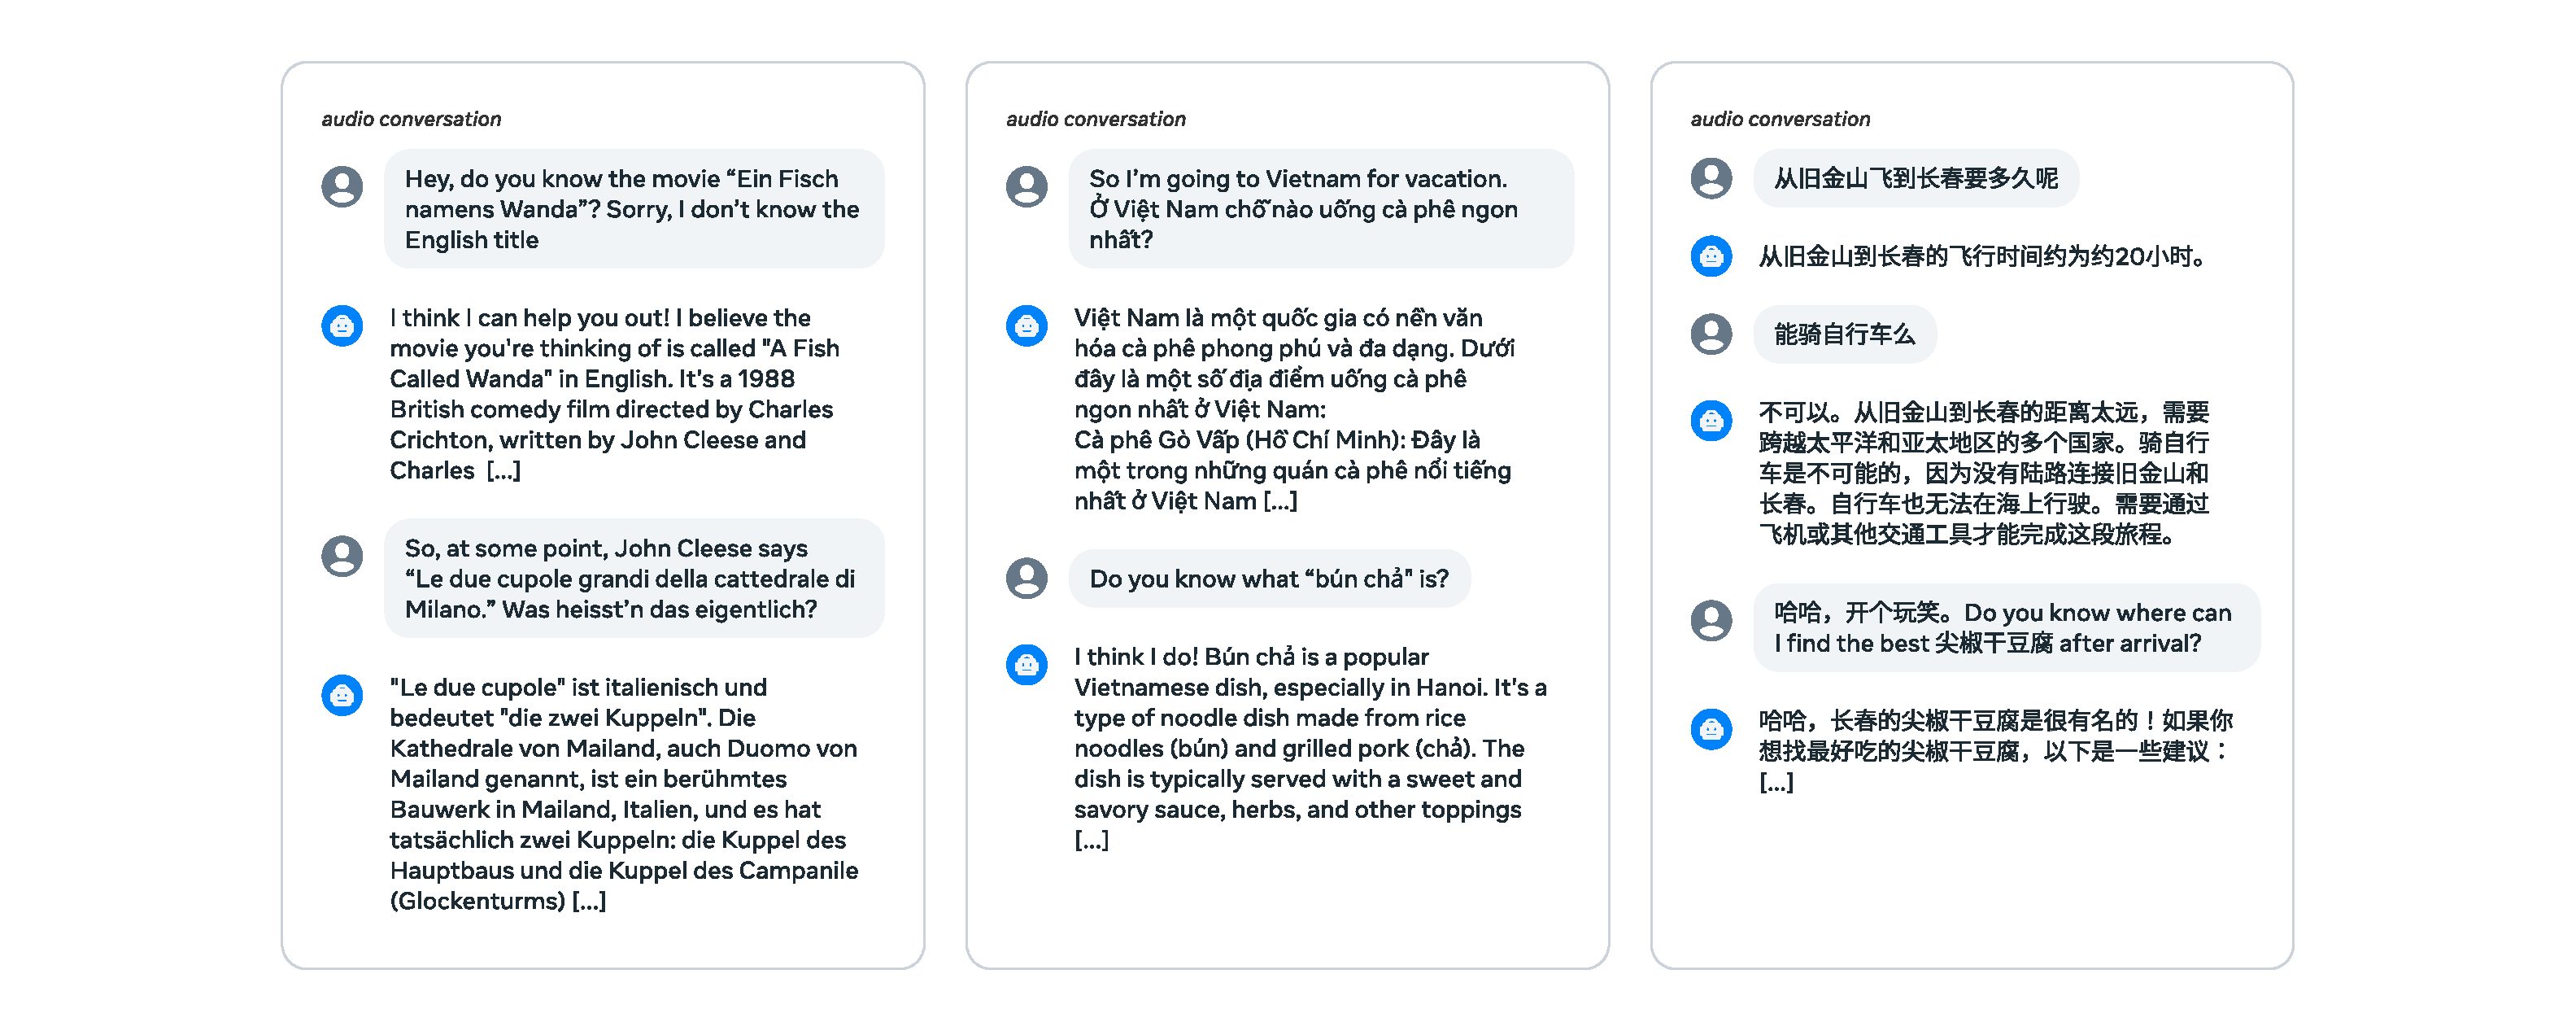
\includegraphics[trim={150px 0 150px 0},clip,width=\textwidth]{assets/llama-voice-language.pdf}
    \caption{\textbf{Transcribed dialogue examples using the speech interface for Llama 3.} The examples illustrate zero-shot multi-turn and code-switching capabilities.}
    \label{figure:speech_dialog_example}
\end{figure}

\textbf{Spoken question answering.}
The speech interface of Llama 3 demonstrates remarkable question answering capabilities. The model can effortlessly comprehend code-switched speech without any prior exposure to such data. Notably, although the model was trained only on single-turn dialogue, it is capable of engaging in extended, coherent multi-turn dialogue sessions.
Figure~\ref{figure:speech_dialog_example} presents a few examples that highlight these multilingual and multi-turn capabilities.

\begin{table}[t]
\centering
    \begin{tabular}{lcccccc}
    \toprule
     & \multicolumn{2}{c}{\textbf{Llama 3 8B}} &  \multicolumn{2}{c}{\textbf{Llama 3 70B}} & \multicolumn{2}{c}{\textbf{Gemini 1.5 Pro}} \\
    \textbf{Language} & AT \bdown & LT \bup & AT \bdown & LT  \bup & AT \bdown & LT \bup \\
    \midrule
    English & 0.84 & 15.09 & \textbf{0.68} & \textbf{15.46} & 1.44 & 13.42 \\
    Overall & 2.31 & 9.89 & \textbf{2.00} & 10.29 & 2.06 & \textbf{10.94} \\
    \bottomrule
    \end{tabular}
    \caption{\textbf{Speech toxicity of our speech interface to Llama 3 on the MuTox dataset.} AT refers to added toxicity (\%) and LT refers to lost toxicity (\%). \label{table:speech-safety-mutox}}
\end{table}

\textbf{Safety.}
We evaluate the safety of our speech model on MuTox \citep{mutox}, a multilingual audio-based dataset of 20,000 utterances for English and Spanish and 4,000 for 19 other languages, each with toxicity labels attached.
The audio is passed as input to the model and the output is evaluated for toxicity, after cleaning some special characters.
We apply the MuTox classifier~\citep{mutox} and compare the results with Gemini 1.5 Pro. We evaluate the percentage of added toxicity (AT), when the input prompt is safe and the output is toxic, and the percentage of lost toxicity (LT), when the input prompt is toxic and the answer is safe. Table~\ref{table:speech-safety-mutox} shows the results for English and an average across all 21 languages that we evaluated on.\footnote{Note that for Gemini, we encountered that a significant number of responses were empty, which could be due to safety filters on their side (though some empty responses were for non-toxic input) or to rate limits. To conduct the analysis, we assumed that all the empty responses are safe. This is the most conservative approach for results and the upper bound of what Gemini results would look like.} The percentage of added toxicity is very low: our speech models have the lowest percentage of added toxicity for English, with less than 1\%. It removes significantly more toxicity than it adds.


\subsection{Speech Generation Results}
For speech generation, we focus on evaluating the quality of token-wise input streaming models with the Llama 3 embeddings for the text normalization and prosody modeling tasks. The evaluation focuses on comparisons with models that do not take the Llama 3 embeddings as an additional input.

\textbf{Text normalization.}
To measure the effect of Llama 3 embeddings, we experimented with changing the amount of right context the model uses. We trained the model using a right context of 3 TN tokens (demarcated by unicode category). This model is compared to models that do not use the Llama 3 embeddings, using a 3-token right context or a full bi-directional context.
As expected, Table~\ref{tab:table1} shows using the full right context improves performance for the model without Llama 3 embeddings. However, the model that incorporates the Llama 3 embeddings outperforms all other models, hence enabling token-rate input/output streaming without relying on long context in the input.

\begin{wraptable}{r}{0.45\textwidth}
	\begin{NiceTabular}{lcc}
		\CodeBefore
		\Body
		\toprule
		\textbf{Model} & \textbf{Context} & \textbf{Accuracy} \\
		\midrule
		Without Llama 3 8B & 3 & 73.6\% \\
		Without Llama 3 8B & $\infty$ & 88.0\% \\
		With Llama 3 8B & 3 & \textbf{90.7\%} \\
		\bottomrule
	\end{NiceTabular}
	\caption{\textbf{Sample-wise text normalization (TN) accuracy.} We compare models with or without Llama 3 8B embeddings, and using different right-context values.\vspace{-8mm}}
	\label{tab:table1}
\end{wraptable}

\textbf{Prosody modeling.}
To evaluate the performance of the our prosody model (PM) with Llama 3 8B, we conducted two sets of human evaluation comparing models with and without Llama 3 embeddings. Raters listened to samples from different models and indicated their preferences. To generate the final speech waveform, we use an in-house transformer based acoustic model \citep{wu2021transformer} that predicts spectral features and a WaveRNN neural vocoder \citep{kalchbrenner2018efficient} to generate the final speech waveform.  %

\begin{table}[t]
	\centering
    \begin{minipage}{.48\textwidth}
      \centering
      \begin{tabular}{lcc}
		\toprule
		\textbf{Model} & \textbf{Preference} \\
		\midrule
		PM for Llama 3 8B  & \textbf{60.0\%} \\
		\small{Streaming phone-only baseline} & 40.0\% \\
		\bottomrule
      \end{tabular}
		\label{tab:tts:pm:ab_test1}
    \end{minipage}\hfill
    \begin{minipage}{.48\textwidth}
      \centering
      \begin{tabular}{lcc}
		\toprule
		\textbf{Model} & \textbf{Preference} \\
		\midrule
		PM for Llama 3 8B & \textbf{63.6\%} \\
		\small{Non-streaming phone-only baseline} & 36.4\% \\
		\bottomrule
      \end{tabular}

    \end{minipage}
    \caption{\textbf{Prosody Modeling (PM) evaluation.} \emph{Left:} Rater preferences of PM for Llama 3 8B vs. streaming phone-only baseline. \emph{Right:} Rater preferences of PM for Llama 3 8B vs. non-streaming phone-only baseline.}
    \label{tab:pm_test}

\end{table}




First, we compare directly to a streaming baseline model without Llama 3 embeddings. 
In  the second test, the Llama 3 8B PM is compared to a non-streaming baseline model without Llama 3 embeddings. 
As shown in Table~\ref{tab:pm_test}, the Llama 3 8B PM is preferred  60\% of the time compared to the streaming baseline, and 63.6\% of the time  compared to the non-streaming baseline, indicating a significant improvement in perceived quality. The key advantage of the Llama 3 8B PM is its token-wise streaming capability (Section~\ref{sec:tts:pm}), which maintains low latency during inference. This reduces the model's lookahead requirements, enabling more responsive and real-time speech synthesis compared to non-streaming baselines.
Overall, the Llama 3 8B prosody model consistently outperforms the baseline models, demonstrating its effectiveness in enhancing the naturalness and expressiveness of synthesized speech.


\paragraph{Functional Magnetic Resonance Imaging Data}

Functional Magnetic Resonance Imaging (fMRI) data are typically represented in four dimensions, indicating the measured blood-oxygen-level-dependent (BOLD) signal in temporal sequences $S = \{V_1, ..., V_t\}$ of 3-dimensional volumes $V \in \mathbb{R}^{x \times y \times z}$, each indicating the BOLD signal for all spatial locations of the brain (as defined by three spatial dimensions $x$, $y$, and $z$). A key challenge for the analysis of fMRI data is the high dimensionality and low sample size of its datasets, which typically contain many hundred thousand dimensions (i.e., voxels) for each of several hundred volumes $V$ in each of tens to hundreds of sequences $S$. In this setting, where the number of features exceed the number of samples, standard machine learning approaches are prone to overfitting.

In spite of the low sample size of individual datasets, neuroimaging research can be considered as recently entering a big data era because researchers more frequently share their collected datasets publicly~\citep{markiewicz_2021_openneuro}. The availability of these data open up the opportunity for pre-training in neuroimaging at scale, as recently demonstrated by~\citep{thomas_fmri_2022}, enabling models to utilize the knowledge that can be learned from public functional neuroimaging data for the analysis of individual datasets. Specifically,~\citep{thomas_fmri_2022} evaluate the performance of several self-supervised learning frameworks for functional neuroimaging data by first pre-training models on a broad fMRI dataset spanning $11,980$ fMRI runs from $1,726$ individuals across $34$ datasets and subsequently adapting the pre-trained models to two downstream mental state decoding datasets (namely, the HCP~\citep{van_2013_wu} and MDTB~\citep{king_2019_functional} datasets). In mental state decoding, predictive models are tasked with identifying (i.e., decoding) some set of mental states (e.g., answering questions about a prose story or math problem) from measured brain activity. The authors find that a GPT-based model, pre-trained in a causal learning framework, performs best in decoding the $20$ (HCP) and $26$ (MDTB) mental states of the two downstream datasets.

To evaluate the performance of H3 on fMRI data, we replicate this analysis, using the up- and downstream fMRI datasets that were published by~\citep{thomas_fmri_2022}, treating H3 as a drop-in replacement for the GPT model. To alleviate the high dimensionality challenge of fMRI data, and due to the generally high spatial correlation of brain activity, the original authors have reduced the volumetric time series $S$ to a set $\Theta \in {\theta_1, ..., \theta_n}$ of $n=1,024$ functionally-independent brain networks $\theta$  (as defined by the dictionaries of functional modes (DiFuMo) brain atlas~\citep{dadi_2020_fine}), each describing the BOLD signal for some subset of voxels $v_{x,y,z} \in V$, such that the resulting sequences $X \in \mathbb{R}^{t \times n}$ describe the activity pattern of each brain network $n$ for time points $t$. 

In line with~\citep{thomas_fmri_2022}, we first pre-train models $f(\cdot)$ to predict the distribution of brain activity for the next time point $j$ of an input sequence $X$, using a mean absolute error ($L_{rec}$) training objective given the model's output $\hat{X} \in \mathbb{R}^{t \times n}$: $L_{rec} = \frac{1}{n} \sum_{i=1}^{n} |X_{j,i} - \hat{X}_{j,i}|$; $\hat{X}_{t,n} = b_n + \sum_n f(E^{X})_{t,e} w_{e,n}$; $E^{X}_{t,e} = E^{TR} + E^{pos} + b_e + \sum_n X_{t,n} w_{n,e}$. Here, $E^{TR} \in \mathbb{R}^{e}$ and $E^{pos} \in \mathbb{R}^{e}$ represent learnable embeddings for each possible time point and position of an input sequence (for details, see~\citep{thomas_fmri_2022}). As the sampling frequency of fMRI is variable, the same position of an input sequence can correspond to different time points. Note that $f(\cdot)$ processes the input in a lower-dimensional embedding representation $E^{X} \in \mathbb{R}^{t \times e}$ (with $e=768$ dimensions).

We evaluate two model architectures for $f(\cdot)$, namely, the GPT variant used in ~\citep{thomas_fmri_2022}, with $4$ hidden layers and $12$ attention heads, and a corresponding H3 variant with $4$ hidden layers (with $H=64$ and $m=1$; see section \ref{sec:method}). For both models, the sequence of hidden-states outputs of the last model layer are used to determine $\hat{X}$.

Just as~\citep{thomas_fmri_2022}, we randomly divide the upstream data into distinct training and validation datasets by randomly designating $5\%$ of the fMRI runs of each of the $34$ upstream datasets as validation data (at a minimum of $2$ runs per dataset) and using the rest of the runs for training. During upstream learning, we then randomly sample sequences of $10$ to $100$ time points from the fMRI runs and train models with the ADAM optimizer (with $\beta_1=0.9$, $\beta_2=0.999$, and $\epsilon=1e^{-8}$ ) for $5,000$ steps at a mini-batch size of $512$, and a learning rate of $5e^{-4}$. We apply a linear learning rate decay schedule (with a warm-up phase of 1\% of the total number of training steps), gradient norm clipping at $1.0$, and $L2$-regularisation (weighted by $0.1$). We also apply dropout at a rate of $0.1$ for the GPT-based model (based on~\citep{thomas_fmri_2022}) and evaluate three dropout rates for H3: $0.1$, $0.2$, and $0.3$. 

\begin{figure}[h]
    \centering
    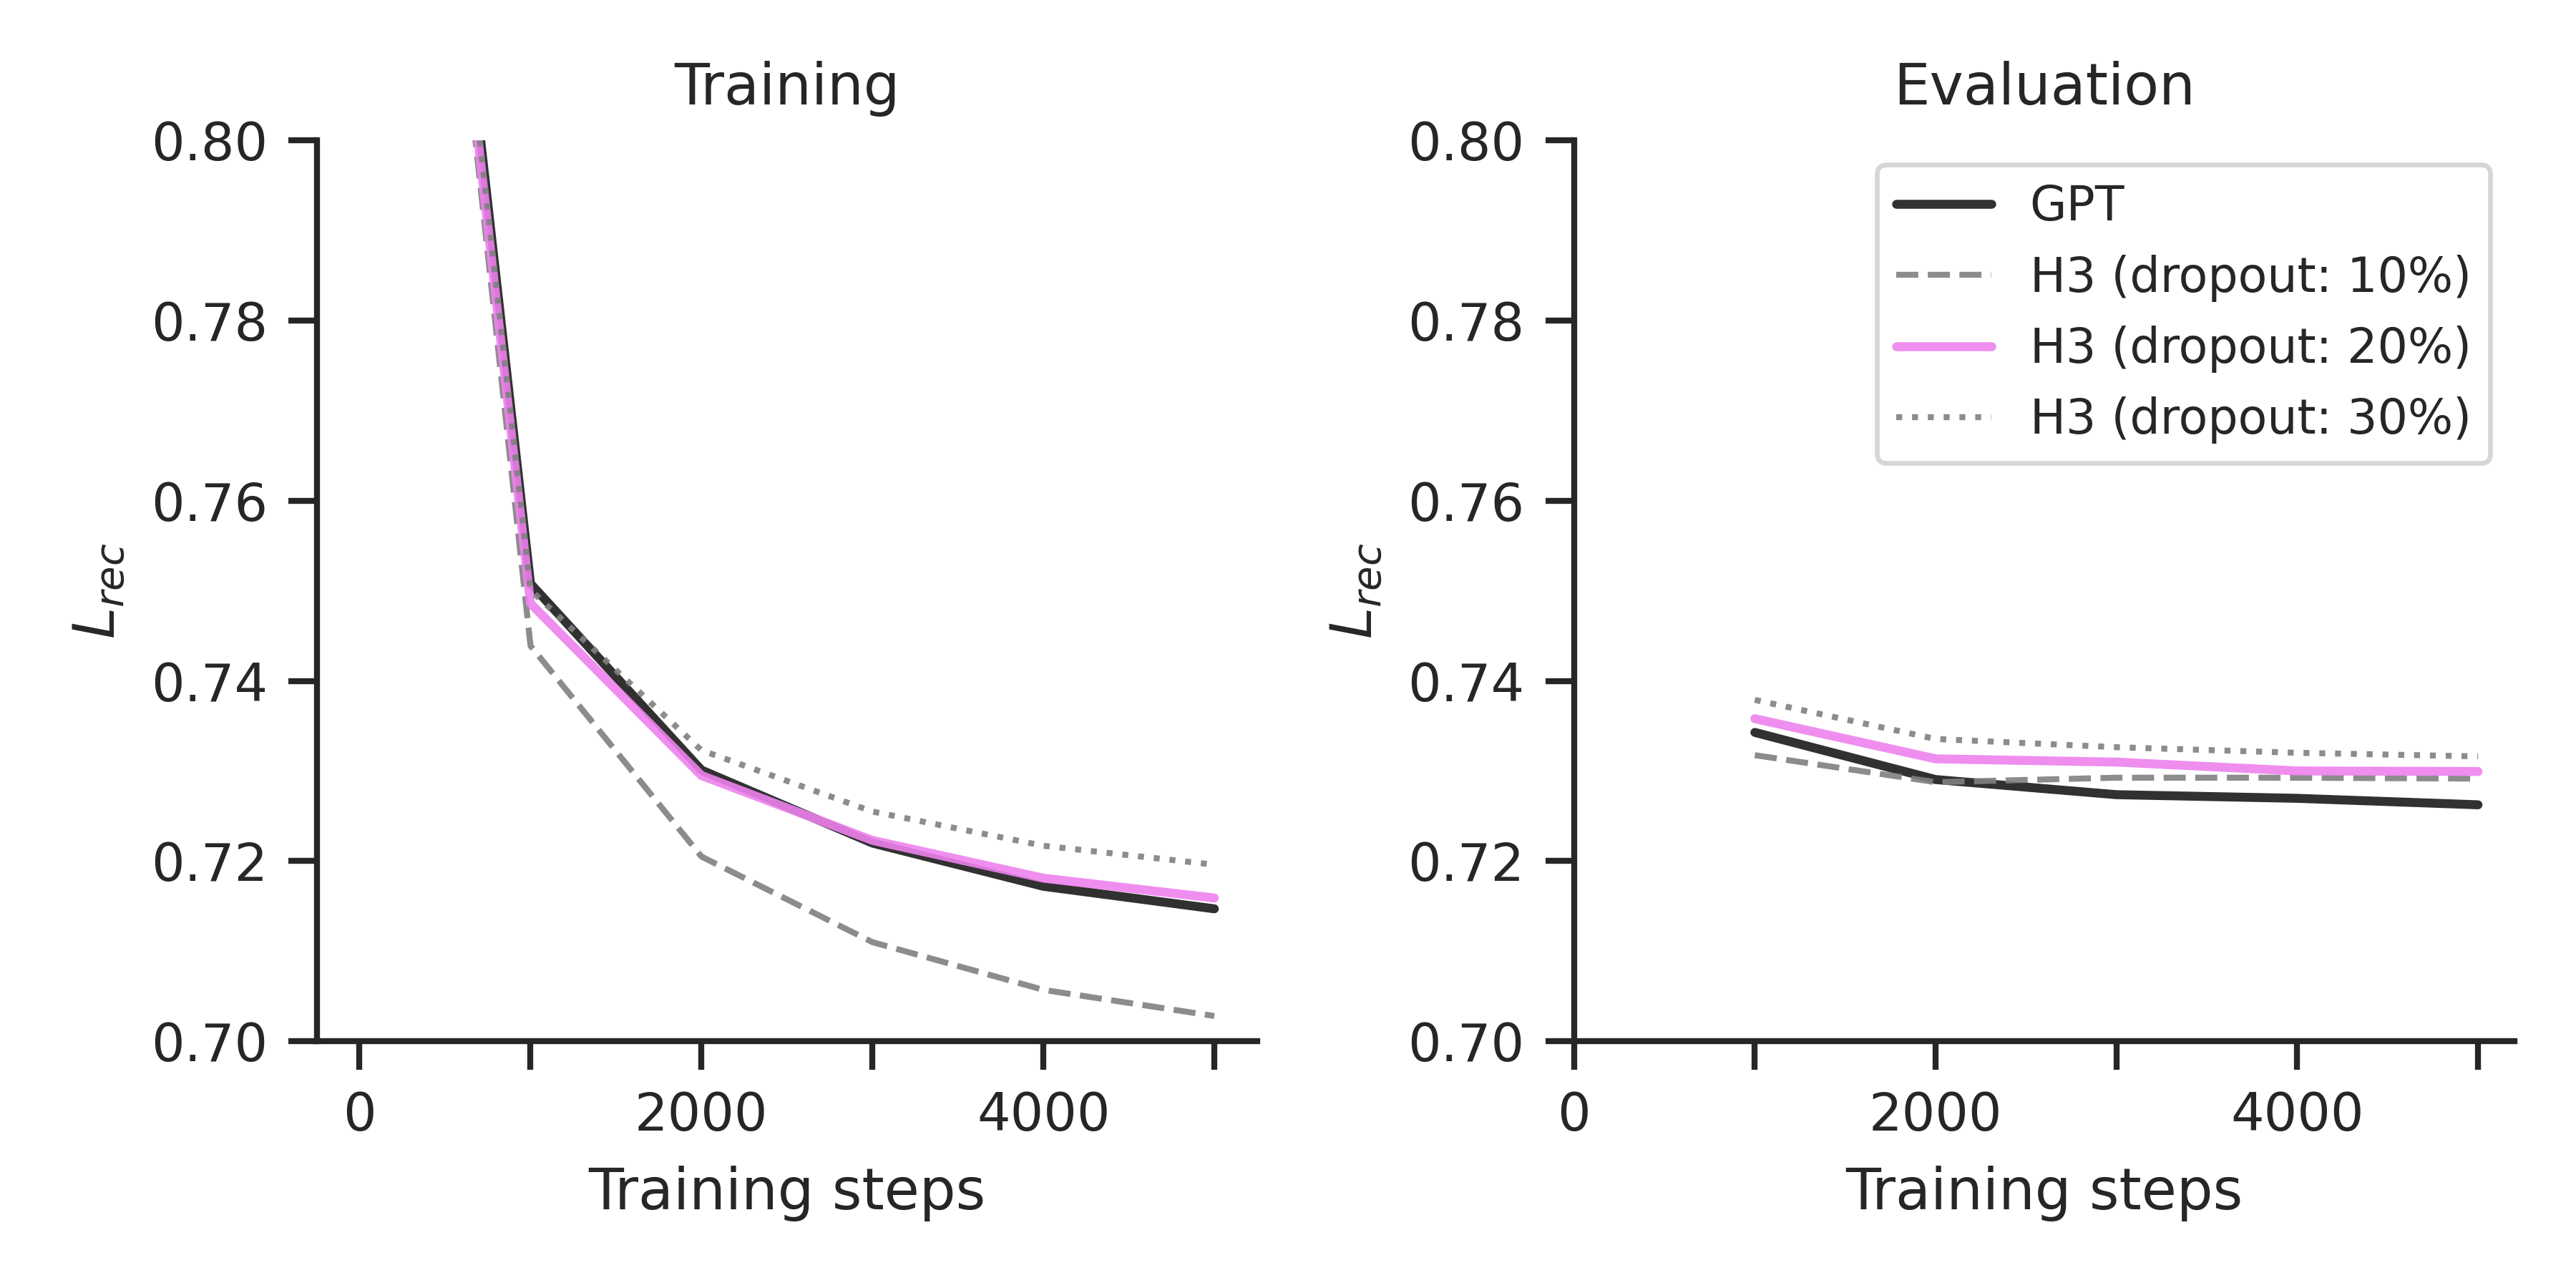
\includegraphics[width=0.65\textwidth]{figs/fmri_upstream-error.png}
    \caption{\label{fig:fmri-upstream} Upstream mean absolute error ($L_{rec}$) in training and evaluation datasets over the course of model training.}
\end{figure}

We find that the H3 variant trained with $0.2$ dropout performs on par with the GPT model, in terms of mean absolute error (Fig.\ \ref{fig:fmri-upstream}), and therefore continue all further analyses with this model variant. We also find that both models exhibit almost identify $L_{rec}$ error distributions throughout the brain, with relatively higher errors in the posterior parietal, occipital, and cingulate cortices as well parts of the limbic system (Fig.\ \ref{fig:fmri-upstream-brain}).

\begin{figure}[h]
    \centering
    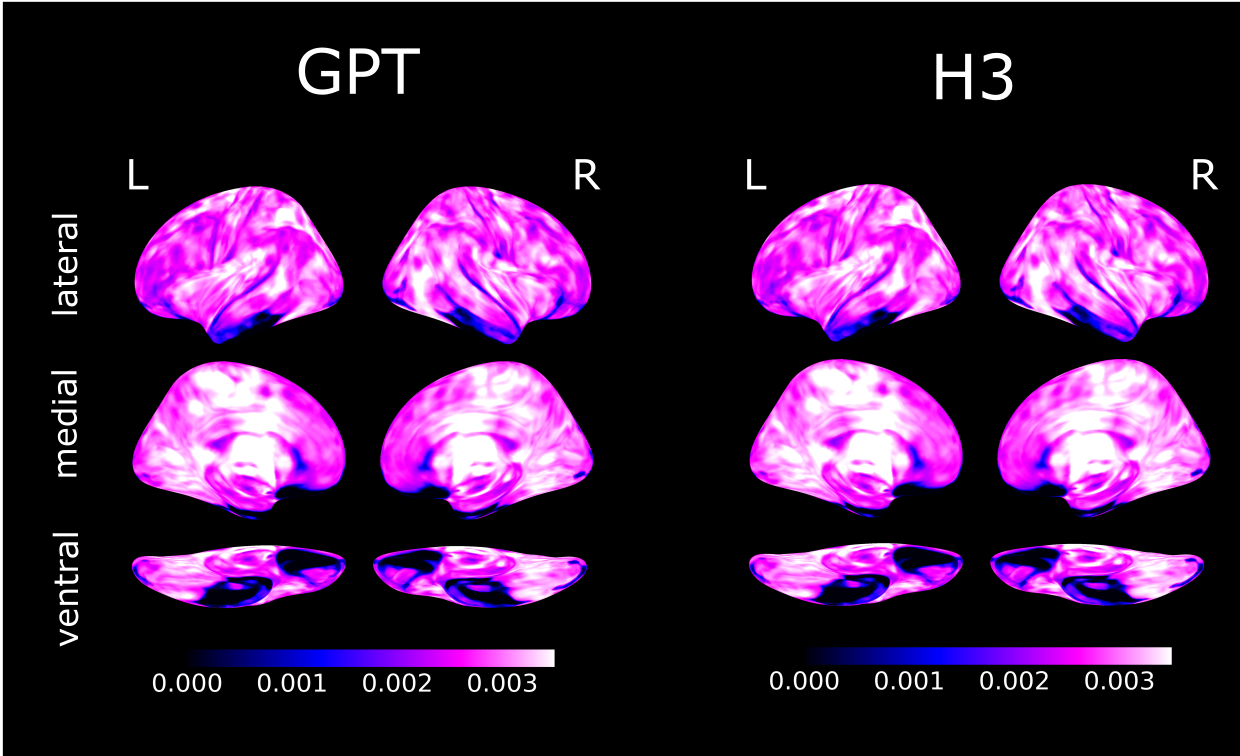
\includegraphics[width=0.5\textwidth]{figs/fmri_upstream-error-brain.png}
    \caption{\label{fig:fmri-upstream-brain} Mean absolute error ($L_{rec}$) of the final pre-trained models for each voxel of the brain projected onto the inflated cortical surface of the FsAverage template~\citep{fischl_2012_freesurfer}.}
\end{figure}

To adapt the pre-trained models to mental state decoding, we add a learnable classification embedding $E^{cls} \in \mathbb{R}^{n}$ to the end of input sequences $X$ and forward the model's prediction $f(E^{X})$ to a decoding head $p(\cdot)$, composed of a dense hidden layer with $e$ model units (one for each embedding dimension, with $tanh$ activation) as well as a $softmax$ output layer with one model unit $i$ for each considered mental state in the data. Accordingly, we adapt models by optimizing a standard cross entropy loss objective: $L_{cls} = - \sum_i y_i \log \ {p(f(E^X))_i}$, where $y_i$ indicates a binary variable that is $1$ if $i$ is the correct mental state and $0$ otherwise.

During downstream adaptation, we begin training with the respective pre-trained model parameters and then allow all parameters to change freely. Similar to~\citep{thomas_fmri_2022}, we randomly split each of the two downstream datasets into distinct training and test datasets, each comprising $40$ (HCP) or $10$ (MDTB) distinct individuals. We adapt models for $750$ steps at a mini-batch size of $256$ and a learning rate of $5e^{-5}$ (otherwise using the same learning parameters as for upstream training). Importantly, we repeat each downstream training run $20$ times using different random seeds, leading to different random splits of the data and variability in other non-deterministic training factors (such as random initialization and data shuffling).

As for the upstream data, the H3 and GPT-based models generally perform on par in their mental state decoding performances in the two left-out test datasets (Table \ref{table:fmri-downstream}).

\begin{table}[h]
    % \captionsetup{font=small}
    \small
    \centering
    %\vspace{-1em}
    \caption{\label{table:fmri-downstream} Downstream adaptation performance of models pre-trained on fMRI data, averaged over $20$ training runs with varying random seeds. F1-scores are macro-averaged.}
    %   \vspace{1em}
    {
        \begin{tabular}{@{}|c|c|cc|@{}}
        %   \specialrule{.15em}{.05em}{.05em}
        \hline
        Dataset & Model & Acc. ($\pm 95\% \text{CI}$) & F1 ($\pm 95\% \text{CI}$)\\ % & Training time \\
        %   \specialrule{.15em}{.05em}{.05em}
        \hline
        HCP & GPT & $88.44$ ($\pm 0.39$) & $87.24$ ($\pm 0.39$) \\
         & H3 & $88.75$ ($\pm 0.33$) & $87.16$ ($\pm 0.37$) \\ \hline
        MDTB & GPT & $89.47$ ($\pm 0.44$) & $88.74$ ($\pm 0.54$) \\
         & H3 & $88.25$ ($\pm 0.45$) & $85.76$ ($\pm 0.61$) \\ \hline
        \end{tabular}
    }
    %\vspace{-1em}
\end{table}

\end{document}
